\documentclass[10pt,a4paper,oneside]{article}
\usepackage[margin=1in]{geometry}
\usepackage[utf8]{inputenc}
\usepackage[english]{babel}
\usepackage{amsmath}
\usepackage{amsfonts}
\usepackage{amssymb}
\usepackage{authblk}
\usepackage{makeidx}
\usepackage{graphicx}
\graphicspath{{./images/}}
\usepackage{float}
\usepackage{listings}
\usepackage{xr-hyper}
\usepackage[breaklinks]{hyperref}
\usepackage{xurl} % best together with hyperref
\usepackage{commath}
\usepackage{bm}
\usepackage[numbers]{natbib}
\usepackage{booktabs}
\usepackage{makecell, caption}
\usepackage{footnote}  
\usepackage{numprint}  
\usepackage{amsthm}
\usepackage{xcolor}
\usepackage{algorithm}
\usepackage{algpseudocode}
\usepackage{fancyvrb}
\usepackage{comment}
\usepackage{mathtools} % Load mathtools package
\usepackage{enumitem} % Required for custom labels and starting numbers
\usepackage{rotating}
\usepackage{longtable}
\usepackage{multirow}
\usepackage{subcaption}

\hypersetup{breaklinks=true}

\newcommand{\U}{\mathbf{U}} 
\newcommand{\J}{\mathbf{J}}
\newcommand{\X}{\mathbf{X}}
\newcommand{\x}{\mathbf{x}}
\newcommand{\M}{\mathbf{M}}
\newcommand{\K}{\mathbf{K}}
\newcommand{\V}{\mathbf{V}}
\newcommand{\W}{\mathbf{W}}
\newcommand{\y}{\mathbf{y}}
\newcommand{\z}{\mathbf{z}} 

\newcommand{\N}{\mathbb{N}}
\newcommand{\Q}{\mathbb{Q}}
\newcommand{\Z}{\mathbb{Z}}
\newcommand{\R}{\mathbb{R}}
\newcommand{\C}{\mathbb{C}}
\newcommand{\Prob}{\mathbb{P}} 
\newcommand{\E}{\mathbb{E}} 
\newcommand{\Sph}{\mathbb{S}} 
\newcommand{\Fil}{\mathbb{F}}

\newcommand{\Al}{\mathcal{A}} 
\newcommand{\Ball}{\mathcal{B}} 
\newcommand{\Sch}{\mathcal{S}} 
\newcommand{\Bo}{\mathcal{L}}
\newcommand{\Hil}{\mathcal{H}}
\newcommand{\SigAl}{\mathcal{F}}

\newcommand{\be}{\bm{\beta}} 
\newcommand{\m}{\bm{\mu}} 
\newcommand{\gm}{\bm{\gamma}} 

\newcommand{\ud}{\,\mathrm{d}}


\newcommand{\iprod}[2]{\langle #1, #2 \rangle}

\newcommand{\rh}[1]{\textcolor{blue}{\textsf{[RH: #1]}}}
\newcommand{\gp}[1]{\textcolor{red}{\textsf{[GP: #1]}}}
\newcommand{\ml}[1]{\textcolor{orange}{\textsf{[M: #1]}}}

\newtheorem{lemma}{Lemma}
\newtheorem{theorem}{Theorem}
\newtheorem{proposition}{Proposition}
\newtheorem*{claim}{Claim}
\newtheorem{definition}{Definition}
\newtheorem{example}{Example}
\newtheorem{remark}{Remark}

\DeclareMathOperator{\esup}{ess\ sup}
\DeclareMathOperator{\spann}{span}
\DeclareMathOperator{\dist}{dist}
\DeclareMathOperator{\support}{supp}
\DeclareMathOperator{\sign}{sign}
\DeclareMathOperator{\perm}{Perm}
\DeclareMathOperator{\concat}{Concat}
\DeclareMathOperator{\sigmoid}{Sigmoid}
\DeclareMathOperator{\LeakyReLU}{LeakyReLU}
\DeclareMathOperator{\batchnorm}{BN}
\DeclareMathOperator{\maxpool}{MP}
\DeclareMathOperator{\zeropad}{ZP}
\DeclareMathOperator{\fullyconnected}{FC}
\DeclareMathOperator{\convolution}{Conv}
\DeclareMathOperator{\lstm}{LSTM}
\DeclareMathOperator{\cnnlstm}{CNNLSTM}
\DeclareMathOperator{\deeplob}{DeepLOB}
\DeclareMathOperator{\argmax}{argmax}
\DeclareMathOperator{\plim}{plim}
\DeclareMathOperator{\var}{Var}



\DeclarePairedDelimiter{\norma}{\lVert}{\rVert} % Define norm notation
\DeclarePairedDelimiter{\aval}{\lvert}{\rvert} % Define absolute value notation


\npthousandsep{,}\npdecimalsign{.}

%\newcommand{\loglik}{\mathcal{l}}
\title{Supplementary Material to Two-Time-Scale Transfer Learning for Market-by-Order Micro-Return Forecasting}
\author[1]{Juan Diego Mejia Becerra}
\author[1]{Gareth W. Peters}
\author[1,2]{Ruimeng Hu}

\affil[1]{Department of Statistics and Applied Probability, University of California, Santa Barbara}
\affil[2]{Department of Mathematics, University of California, Santa Barbara}


\date{Last Modified: \today}

\makeatletter
\let\oldbibcite\bibcite
\def\bibcite#1#2{}
\externaldocument{build/paper_draft}
\let\bibcite\oldbibcite
\makeatother

\begin{document}

\maketitle

\tableofcontents
\clearpage


\appendix

\section{Mathematical Representation of the Order Flow Sequence and Limit Order Book}
\label{ap:matreplob}


This section is devoted to mathematically describing the OF sequence and the LOB drawing ideas from \cite{cont2023mathematical, gould2013limit, panayi2015stochastic}. First observe that most LOBs operate with a minimum price variation, or tick size, denoted $\theta$, and a maximum price, denoted $D$. For simplicity, and without losing generality, prices will be measured in ticks. Also let $d = \frac{D}{\theta} \in \N \setminus \{ 0 \}$ be the maximum price measured in ticks and denote $\N_{0:d} = \{ 0, 1, \dots, d\}$ the set of possible tick-measured prices.

\begin{definition}
    Let $o = (p_o, z_o, t_o, i_o, s_o, k_o)$ denote a message submitted to the matching engine at time $t_o \in [0, T]$, with price $p_o \in \N_{0:d}$, size $z_o \in \N$, identifier $i_o \in \N$, side $s_o \in \{1, -1\}$ and type $k_o \in \{L, C, M \}$. $s_o = 1$ ($s_o = -1$) indicates that the message $o$ is submitted in the bid (ask) side of the LOB. $L$, $C$ and $M$ identify limit, cancellations and market orders respectively. 
    \label{def:order}
\end{definition}

\begin{definition}
    Let $\mathbf{o} = \{o_i\}^{N - 1}_{i = 1} $, $N \in \N$, denote an ordered sequence of messages such that $t_{o_i} \leq t_{o_{i + 1}}$. This sequence is known as the order flow sequence.
\label{def:order_seq}
\end{definition}

To favor notation lightness, The subscript $o_i$ will be dropped in favor of $i$ in the elements of the message sequence $\mathbf{o}$ whenever no ambiguity is present (e.g. $t_i$ instead of $t_{o_i}$ will be used). For simplicity, identify buy (sell) market orders in the order sequence $\mathbf{o}$ as limit orders with the maximum (minimum) possible price. That is, 

\begin{align*}
    (p_o, z_o, t_o, i_o, 1,  M) &\equiv (d, z_o, t_o, i_o, 1, L) \\
    (p_o, z_o, t_o, i_o, -1, M) &\equiv (0, z_o, t_o, i_o, -1, L)
\end{align*}


\begin{definition}
Let $d \in \N \setminus \{ 0 \}$ be the maximum price of an asset. The order aggregator, $\mathcal{X} : \N \times \N \times [0, T] \times \N \times \{-1, 1 \} \times \{ L, C\} \rightarrow \Z^d \times \Z^d$, groups limit orders and cancellations by price and adds its sizes
    
$$
\mathcal{X}(\mathbf{o}) = \left( \sum_{o \in \mathbf{o}} (I^+_L(o) - I^+_C(o)) z_o e_{p_o}, \sum_{o \in \mathbf{o}} (I^-_L(o) - I^-_C(o)) z_o e_{p_o} \right),
$$
where the market orders in $\mathbf{o}$ are identified as limit orders, $e_i = (0, 0, \dots, 0, 1, 0, \dots, 0) \in \Z^d$ where 1 is the $i$-th position, $I^+_k(o)$ ($I^-_k(o)$) takes value $1$ if $s_o = 1$ ($s_o = -1$) and $k_o = k$, $k \in \{ L, C\}$.
\label{def:order_aggregator}
\end{definition}


Two pathological scenarios might arise with the established notation. First, a cancellation message might exceed the size of the initial order or target a nonexistent order, inadvertently transforming into a market order that could circumvent the established price-time priority rules. Second, a single order could deplete all available liquidity on the opposite side of the LOB, leading to a situation where the price becomes undefined. Although these scenarios are rare, occurring under highly specific conditions, we preclude them by setting forth two basic assumptions:

\begin{itemize}
    \item[(A1)] Every cancellation correspond to a message submitted earlier, with no cancellation exceeding the outstanding size 
    \item[(A2)] No buy (sell) market order exceeds the ask (bid) volume of the limit order book.
\end{itemize}

The set of possible values of $\mathbf{o}$ under the restrictions (A1) and (A2) is denoted as $\mathcal{O}$. To reconstruct the LOB, the modular framework described in \cite{cont2023mathematical} is employed. This framework decomposes the dynamics of the limit order book into two distinct elements: the incoming order flow and the market clearing procedure. The incoming order flow is conceptualized as a marked point process, while the market clearing procedure is a deterministic operator responsible for pairing buy and sell orders.


Denote $X = (X^+, X^-) \in E := \N^d \times \N^d$ a configuration of limit orders.\footnote{i.e. $X = \mathcal{X}(\mathbf{x})$ for some $\mathbf{x} \in \mathcal{O}$.}  Observe that the set of valid configurations of LOBs is a proper subset of $E$. Some notation is necessary to determine this set. First, for $Z \in \N^d$, consider the measure 

$$
\nu_Z = \sum^d_{k = 1}Z_k \delta_k,
$$
where $\delta_k$ denotes the Dirac's delta measure at $k \in \{1, \dots, d \}$. Also, let

\begin{itemize}
    \item $\nu^{\pm}_X = \nu_{X^{\pm}}$
    \item $\tau^i(Z)$ be such that $\nu_{\tau^i(Z)} = \nu_Z 1_{[i, \infty)}$
    \item $\tau_i(Z)$ be such that $\nu_{\tau_i(Z)} = \nu_Z 1_{[0, i]}$
    \item $a(X) = \inf \support(\nu^+_{X})$, with $a(0) = 0$
    \item $b(X) = \sup \support(\nu^-_{X^+})$, with $b(0) = d$
\end{itemize}

Observe that $a(X)$ and $b(X)$ correspond to the best ask and bid of a limit order book snapshot respectively. The set of valid limit order book configurations is thus

$$
\Bo := \{X = (X^+, X^-) \in E : a(X) > b(X)\}.
$$

\begin{definition}
    Let $\mathbf{o} \in \mathcal{O}$. Define the mapping $J : [0, T] \times \mathcal{O} \rightarrow \Z^d \times \Z^d$ as follows

    \begin{equation*}
    J(t, \mathbf{o}) = \begin{cases}
        \mathcal{X}(\{ o \in \mathbf{o} : t_o = t_i  \}) & \text{if } t = t_{i} \ \exists  i = 1, \dots, N,\\
        0                        & \text{otherwise.}
    \end{cases}
\end{equation*}
    
\end{definition}

Observe that $J$ models changes in the LOB right before matching. The matching process is modeled in \cite{cont2023mathematical} through a deterministic order matching clearing operator $\mathcal{C} : E \rightarrow \Bo$ whose set of invariant points is $\Bo$. It can be shown that, under some conditions, $\mathcal{C}$ is uniquely characterized as follows:

\begin{equation*}
    \mathcal{C}(X)^+ = \begin{cases}
        \tau_{p_B(X)}(X^+)                                       & \text{if } g_X(p_B(X)) \leq - X^+_{p_B(X)}, \\
        \tau_{p_B(X) - 1}(X^+) - \min(0, g_X(p_B(X))) e_{p_B(X)} & \text{if } g_X(p_B(X)) > - X^+_{p_B(X)}.
    \end{cases}
\end{equation*}

\begin{equation*}
    \mathcal{C}(X)^- = \begin{cases}
        \tau^{p_A(X)}(X^-)                                       & \text{if } g_X(p_A(X)) \geq X^-_{p_A(X)}, \\
        \tau^{p_A(X) + 1}(X^-) + \max(0, g_X(p_A(X))) e_{p_A(X)} & \text{if } g_X(p_A(X)) <  X^-_{p_A(X)},
    \end{cases}
\end{equation*}
where $X \in E$ is the set of limit orders. Let $B_X(k) = \nu^+[k, \infty)$, $S_X(k) = \nu^-_X[0, k]$, $g(k) = S_X(k) - B_X(k)$, and
\begin{align*}
    p_A(X) = \inf \{ k \in \{1, \dots, d \} : g_X(k) > 0 \},\\
    p_B(X) = \sup \{ k \in \{1, \dots, d \} : g_X(k) < 0 \}.
\end{align*}
The reconstruction of an LOB given $\mathbf{o} \in  \mathcal{O}$ is now straightforward:

\begin{definition} Given $\mathbf{o} \in \mathcal{O}$, the reconstructed LOB is a mapping $L : [0, T] \times \mathcal{O} \rightarrow \Bo$ such that 

\begin{equation*}
    L(t, \mathbf{o}) =\begin{cases}
        L(t_*, \mathbf{o}) & if \ t \neq t_i\ \forall i = 1, \dots, N,\\
        \mathcal{C}\left( L(t_*, \mathbf{o}) + J(t_i, \mathbf{o}) \right) & if \ t = t_i \ \exists i = 1, \dots, N.
    \end{cases}
    \label{def:LOB_reconstructor}
\end{equation*}
Here, $t_* = \max\{t_j : t_j < t\}$.
\end{definition}

\begin{definition}
    For a valid LOB configuration, $X \in \mathcal{L}$, let $b_h(X) = b(X) - h$ ($a_h(X) = a(X) + h$) be the price $h$ ticks below (above) the best bid (ask).
     Also let $V^b_h(X) = \nu^+_{X}\{b_{h}(X)\}$ ($V^a_h(X) = \nu^-_{X}\{a_{h}(X)\}$) be the corresponding volume sitting $h$ ticks below (above) the best ask. For convenience, denote $a_h(t) = a_h(X(t))$, $b_h(t) = b_h(X(t))$, $V^a_h(t) = V^a_h(X(t))$ and $V^b_h(t) = V^b_h(X(t))$.
     \label{def:bid_ask_volume_dephts}
\end{definition}

An alternative approach, known as the compressed representation, to describe the liquidity available in the LOB is in terms of its levels. The $l$-th bid (ask) price level is defined as the $l$-th highest (lowest) price in the LOB that has positive volume available. Formally, 

\begin{definition}
    For a valid LOB configuration, $X \in \mathcal{L}$, the $l$-th level bid (ask) price, is defined iteratively as $p^b_l(X) = \inf \support\left(\tau_{p^b_{l - 1}(X) - 1}(X^+) \right)$ ($p^a_l(X) = \inf \support\left(\tau^{p^a_{l - 1}(X) + 1}(X^-) \right)$) for $l \geq 1$ and $p^b_0(X) = b_0(X)$ ($p^a_0(X) = a_0(X)$). Similarly, denote the volume available at the $l$-th bid (ask) level as $v^b_l(X) = \nu^+_{X}\{p^b_l(X)\}$ ($v^a_l(X) = \nu^-_{X}\{p^a_l(X)\}$). To keep notation light, denote $p^a_l(t) = p^a_l(X(t))$, $p^b_l(t) = p^b_l(X(t))$, $v^a_l(t) = v^a_l(X(t))$ and $v^b_l(t) = v^b_l(X(t))$.
    \label{def:bid_ask_volume_levels}
\end{definition}

Each representation offers distinct trade-offs. For instance, working with decompressed limit order book data may simplify the mathematical modeling of order flow, while compressed formats are more memory-efficient—an especially important advantage for illiquid assets. Moreover, compressed representations often provide a more suitable input to neural network models, potentially enhancing their predictive accuracy.


We have assumed a fixed message sequence $\mathbf{o} \in \mathcal{O}$ and reconstructed the limit order book for such sequence. To add stochasticity, let $(\Omega, \SigAl, \Fil, \Prob)$ be a filtered, complete and right-continuous probability space and consider the following 

\begin{definition}
Let $\tau$ be a $\Fil$-stopping time and $\pi$, $\zeta$, $\iota$, $\sigma$ and $\kappa$; $\SigAl_{\tau}$-adapted random variables with values in $\N_{0:d}$, $\N$, $\N$, $\{-1, 1\}$, and $\{L, C, M\}$ respectively. The corresponding stochastic message is denoted as  $\omega = (\pi, \zeta, \tau, \iota, \sigma, \kappa)$.

Analogously, for a sequence of non-explosive increasing sequence of $\Fil$-adapted stopping times $(\tau_i)^{\infty}_{i = 1}$ and $\SigAl_{\tau_i}$-measurable random variables $\pi_i$, $\zeta_i$, $\iota_i$, $\sigma_i$, and $\kappa_i$ for which assumptions (A1) and (A2) hold, define the stochastic message sequence

\begin{equation*}
\boldsymbol{\omega} = (\omega_i : \tau_i \leq T),
\end{equation*}
where $\omega_i = (\pi_i, \zeta_i, \tau_i, \iota_i, \sigma_i, \kappa_i)$. 
\label{def:stochastic_messages}
\end{definition}

The $L$ function from definition \ref{def:LOB_reconstructor} can be employed to specify a stochastic LOB.

\begin{definition} The LOB process is a stochastic process, denoted $(X(t))_{t \geq 0}$ and defined as

\begin{equation*}
X(t) = L(t, \boldsymbol{\omega}).
\end{equation*}
\label{def:lob_process}
\end{definition}

For the sake of clarity, the previous definitions are illustrated below. Consider the following order flow sequence $\mathbf{o} \in \mathcal{O}$ represented in the following table

\begin{table}[H]
  \caption{Example OF sequence}
  \label{tab:of_example}

\centering
\begin{tabular}{cccccc}
\hline
$p_i$ & $z_i$ & $t_i$ & $i_i$ & $s_i$ & $k_i$ \\ \hline
10    & 10   & 0.04      & 1          & 1    & L    \\
11    & 20   & 1.23      & 2          & 1    & L    \\
12    & 100  & 2.45      & 3          & -1   & L    \\
12    & 50   & 3.14      & 4          & -1   & L    \\
8     & 50   & 4.75      & 5          & -1   & L    \\
9     & 150  & 5.63      & 6          & 1    & L    \\
13    & 30   & 6.14      & 7          & 1    & L    \\
13    & 45   & 7.85      & 8          & -1   & L    \\
12    & 70   & 8.32      & 3          & -1   & C    \\
12    & 50   & 9.78      & 4          & -1   & C    \\ \hline
\end{tabular}

\end{table}

Definition~\ref{def:order_aggregator} applied to the sequence $\mathbf{o}$ implies

\begin{align*}
    \mathcal{X}(\mathbf{o}) = &\big(150 e_{9} + 10 e_{10} + 20 e_{11} + 30 e_{13}, \\
                               &\hspace{5mm} 50 e_8 + 30 e_{12} + 45 e_{13}\big).
\end{align*}
This object is depicted in Figure~\ref{fig:uncleared_example_orders}.

\begin{figure}[h!]
    \centering
    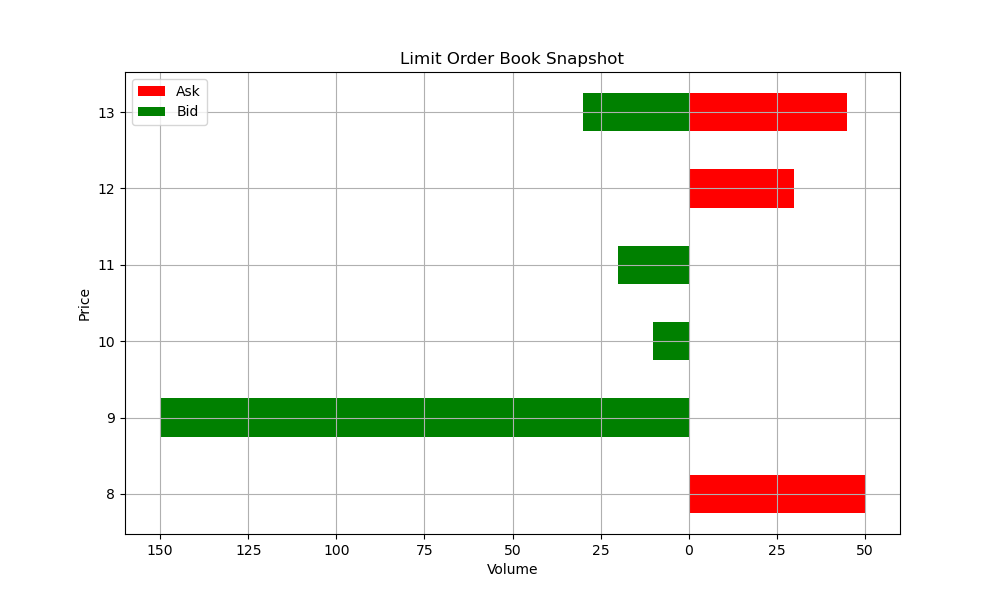
\includegraphics[height=2.5in]{uncleared_example_lob.png}    
    \caption{Aggregated example orders.}
    \label{fig:uncleared_example_orders}
\end{figure}

Following the price-time priority rule, orders 1 through 4 are not marketable and are simply added to the LOB. The aggressive sell order 5 then arrives, clearing orders 1 and 2 entirely and leaving 20 units unexecuted on the ask side sitting at 8 ticks, with the bid side empty. When the buy order 6 arrives, it clears the remaining 20 units of order 5, leaving 130 units on the bid side sitting at 9 ticks. Order 7 next clears 30 units of order 3, leaving 120 units at 12 ticks on the ask side. Another 45 units are then added at price 13 on the ask side. Finally, messages 9 and 10 cancel the remaining volumes of orders 3 and 4. Thus leaving 130 units sitting on the bid side at 9 ticks and 45 units sitting at 13 ticks on the ask side. As a side note, observe that $\mathcal{C}\left( \mathcal{X}(\mathbf{o}) \right) = \left( 150 e_9 + 10 e_{10}, 30 e_{12} + 45 e_{13} \right)$ which is different from the resulting LOB of the example $L(t = 10, \mathbf{o}) = (130 e_9, 45 e_{13})$. This reflects the fact that continuously clearing the LOB (as in trading hours) can yield different results to discrete clearing (as in opening/closing auctions).

Figure~\ref{fig:snapshot_seq} illustrates the corresponding sequence of LOB snapshots resulting from these events.

\begin{figure}[h!]
    \centering
    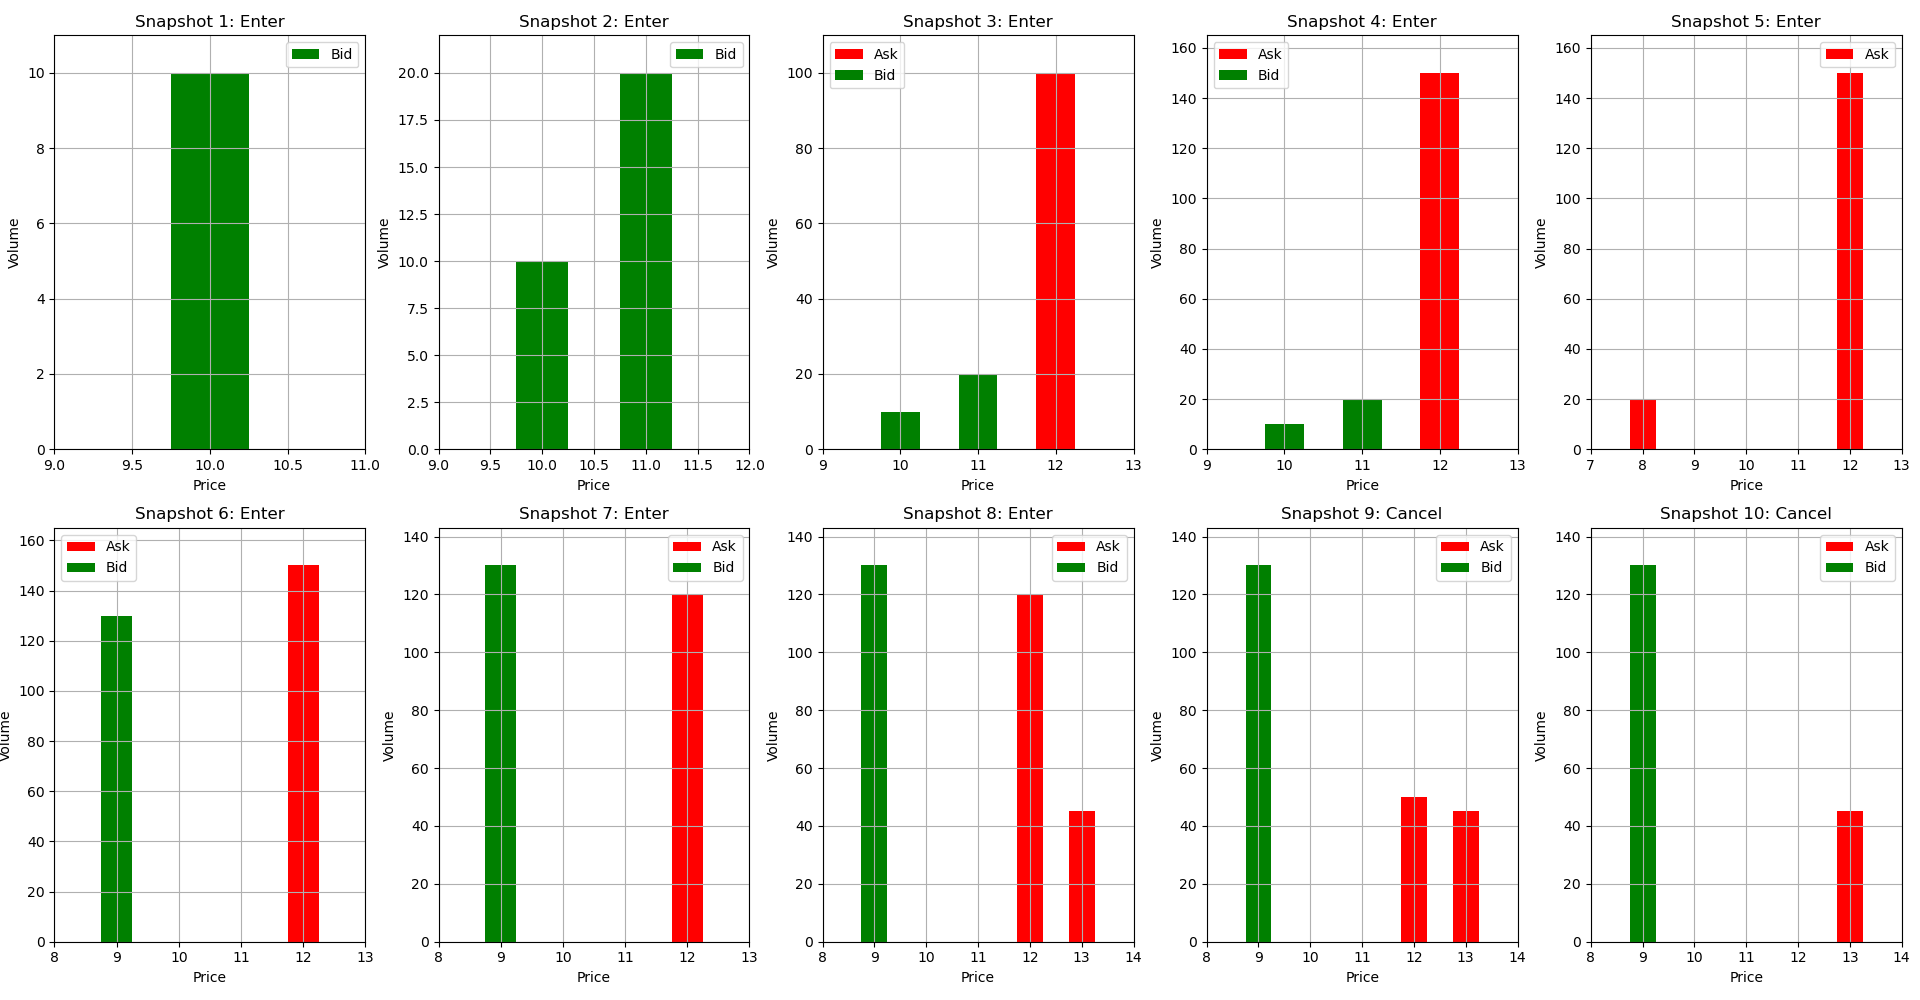
\includegraphics[height=3in]{lob_snapshot_sequence.png}    
    \caption{Sequence of LOB snapshots corresponding to Table \ref{tab:of_example}.}
    \label{fig:snapshot_seq}
\end{figure}

A useful distinction between the OF sequence and MBO data lies in how MBO data can be constructed from the OF sequence without requiring explicit order matching. One way to achieve this is by labeling addition messages as \verb|A| and cancellation messages as \verb|C|. Whenever an outstanding order executes, a series of messages—\verb|T| (trade), \verb|F| (filled), and \verb|C| (cancellation)—can be inserted at the same timestamp to indicate the trade initiator, the filled order, and the final cancellation needed for LOB reconstruction. Under this scheme, the LOB can be fully reconstructed using only \verb|A| and \verb|C| messages, eliminating the need for a separate clearing process. Table \ref{tab:mbo_data} illustrates this procedure.

\begin{table}[H]
  \caption{Example MBO data.}
  \label{tab:mbo_data}

\centering
\scalebox{0.75}{
\begin{tabular}{c c c c c c c}
\hline
\textbf{timestamp} & \textbf{order\_id} & \textbf{side} & \textbf{volume} & \textbf{price} & \textbf{message\_type} \\
\hline
0.04 & 1 & B   & 10  & 10 & A \\
1.23 & 2 & B   & 20  & 11 & A \\
2.45 & 3 & A   & 100 & 12 & A \\
3.14 & 4 & A   & 50  & 12 & A \\
4.75 & 5 & A   & 20  & 11 & T \\
4.75 & 2 & B   & 20  & 11 & F \\
4.75 & 2 & B   & 20  & 11 & C \\
4.75 & 5 & A   & 10  & 10 & T \\
4.75 & 1 & B   & 10  & 10 & F \\
4.75 & 1 & B   & 10  & 10 & C \\
4.75 & 5 & A   & 20  & 8  & A \\
5.63 & 6 & B   & 20  & 8  & T \\
5.63 & 5 & A   & 20  & 8  & F \\
5.63 & 5 & A   & 20  & 8  & C \\
5.63 & 6 & B   & 130 & 9  & A \\
6.14 & 7 & B   & 30  & 12 & T \\
6.14 & 3 & A   & 30  & 12 & F \\
6.14 & 3 & A   & 30  & 12 & C \\
7.85 & 8 & A   & 45  & 13 & A \\
8.32 & 3 & A   & 70  & 12 & C \\
9.78 & 4 & A   & 50  & 12 & C \\
\hline
\end{tabular}}

\end{table}

\clearpage
\section{Alternative Sampling Schemes}
\label{ap:sampling_schemes}
For completeness, we define the \emph{volume bars} partition \(\mathcal{P}^{(V)}\) via the stopping times
\[
\tau^{(V)}_i \;=\;\inf\Bigl\{\,t>\tau^{(V)}_{i-1}:\sum_{k:\,\kappa_k=M}\zeta_k>i\cdot\texttt{Vol}\Bigr\},\quad \tau^{(V)}_0=0,
\]
where \(i,\texttt{Vol}\in\mathbb{Z}^+\). Each interval \(\Delta\tau^{(V)}_i \;=\;\tau^{(V)}_i-\tau^{(V)}_{i-1}\) corresponds to the time required for \(\texttt{Vol}\) units to trade. Furthermore, given any partition \(\mathcal{P}\), we define the counting process
\[
N^{\mathcal{P}}(t)\;=\;\left|\bigl\{\tau\in\mathcal{P}:\,0<\tau\le t\bigr\} \right|,
\]
such that \(N^{\mathcal{P}}(t_1,t_2) = N^{\mathcal{P}}(t_2)-N^{\mathcal{P}}(t_1)\) counts the number of partition points in \((t_1,t_2]\).

\clearpage
\section{CNN–LSTM and DeepLOB Model Specifications}
\label{ap:nn_specs}

This section formalizes the CNN–LSTM and DeepLOB architectures \cite{kolm2023deep, Zhang_2019}.  Section~\ref{subsec:building_blocks} introduces the fundamental tensor operations, which are assembled into the composite layers described in Section~\ref{subsec:composite_structures}.  These composite layers are then connected via convolutional and inception modules to yield the full CNN–LSTM and DeepLOB architectures, as detailed in Section~\ref{subsec:nn_architectures}.

\subsection{Building Blocks}
\label{subsec:building_blocks}

This section describes the fundamental tensor operations that compose the CNN-LSTM and DeepLOB architectures. 

\subsubsection{Permutation}

For simplicity, consider a tensor $T \in \mathbb{R}^{N_1 \times N_2 \times \cdots \times N_d}$ as a multidimensional array with entries denoted by $T_{i_1 i_2 \cdots i_d}$. Denote the data batches as four-dimensional tensors in \(\mathbb{R}^{N \times C \times H \times W}\), where \(N\) denotes the batch size, \(C\) the number of channels, \(H\) the temporal length, and \(W\) the spatial width.

Tensor permutation serves as a higher-dimensional analogue to the matrix transpose. Define the permutation between the $k$-th and $l$-th dimensions as 

\begin{align*}
    \perm^{k, l}: \R^{N_1 \times N_2 \times \cdots \times N_k \times \cdots \times N_l \times \cdots \times N_d} &\rightarrow \R^{N_1 \times N_2 \times \cdots \times N_l \times \cdots \times N_k \times \cdots \times N_d}\\
    T &\mapsto \perm^{k, l}(T)
\end{align*}
where $\bigl[\perm^{k, l}(T)\bigr]_{i_1 i_2 \cdots i_k \cdots i_l \cdots i_d} = T_{i_1 i_2 \cdots i_l \cdots i_k \cdots i_d}$. 

\subsubsection{Concatenation}

Tensor concatenation along the $k$-th dimension is defined as

\begin{align*}
    \concat^k : \mathbb{R}^{N_1 \times N_2 \times \cdots \times N_k \times \cdots \times N_d} \times \mathbb{R}^{N_1 \times N_2 \times \cdots \times N'_k \times \cdots \times N_d} &\rightarrow \R^{N_1 \times N_2 \times \cdots \times (N_k + N'_k) \times \cdots \times N_d}\\
    (T, S) &\mapsto \concat^k(T, S)
\end{align*}
where,

$$
\bigl[\concat^k(T, S)\bigr]_{i_1 i_2  \cdots i_k \cdots i_d} = \begin{cases}
    T_{i_1 i_2 \cdots i_k \cdots i_d} & 1 \leq i_k \leq N_k,\\
    S_{i_1 i_2 \cdots i_k \cdots i_d} & N_k + 1 \leq i_k  \leq N_k + N'_k.
\end{cases}
$$


\subsubsection{Activation Functions}

Two activation functions are necessary: The Sigmoid and the Leaky RelU. For a scalar $x \in \R$ these two activation functions are defined as

\begin{align*}
    \sigmoid(x) &= \frac{1}{1 + \exp(-x)},\\
    \LeakyReLU_{\alpha}(x) &= \begin{cases}
        x & x \geq 0,\\
        \alpha x & x < 0.
    \end{cases}
\end{align*}
For a tensor $T \in \R^{N_1 \times N_2 \times \cdots \times N_d}$, define $\sigmoid: \R^{N_1 \times N_2 \times \cdots \times N_d} \rightarrow \R^{N_1 \times N_2 \times \cdots \times N_d}$  and $\LeakyReLU_{\alpha}: \R^{N_1 \times N_2 \times \cdots \times N_d} \rightarrow \R^{N_1 \times N_2 \times \cdots \times N_d}$

\begin{align*}
    \bigl[\sigmoid(T)\bigr]_{i_1 i_2 \cdots i_d} &= \sigmoid(T_{i_1 i_2 \cdots i_d}),\\
    \bigl[\LeakyReLU_{\alpha}(T)\bigr]_{i_1 i_2 \cdots i_d} &= \LeakyReLU_{\alpha}(T_{i_1 i_2 \cdots i_d}).
\end{align*}

\subsubsection{Batch Normalization}

In the CNN-LSTM model, Spatial Batch Normalization, PyTorch’s \texttt{BatchNorm2d}\footnote{\url{https://pytorch.org/docs/stable/generated/torch.nn.BatchNorm2d.html} (Accessed on 04-29-2025)}, originally proposed in \cite{ioffe2015}, is applied to each convolutional feature map. For a tensor of size $N$ and feature maps of shape $(C,H,W)$, \texttt{BatchNorm2d} computes per-channel statistics over all $N\times H\times W$ activations, then learns one pair of affine parameters $(\gamma_c,\beta_c)$. This normalization is supposed to alleviate the internal covariate shift problem by fixing each channel’s mean to zero and variance to one. This stabilization has been empirically shown to allow for higher learning rates and faster convergence, and can indirectly alleviate issues like vanishing or exploding gradients. 

More precisely, let $T\in\mathbb{R}^{N\times C\times H\times W}$ denote an activation tensor of size $N$ each with $C$ channels of spatial size $H\times W$.  Denote by $T_{icjk}$ the element for sample $i$, channel $c$, and spatial position $(j,k)$. The Spatial Normalization operation is an application $BN^{\phi, \varepsilon} : \R^{N \times C\times H\times W} \rightarrow \R^{N \times C\times H\times W}$ defined as 

\[
\bigl[\batchnorm^{\phi, \varepsilon}(T)\bigr]_{icjk}
= \gamma_c \, \frac{T_{icjk} - \mu_c}{\sqrt{\sigma_c^{2} + \varepsilon}} + \beta_c.
\]
Here, $\gamma_c$ and $\beta_c$ are trainable parameters, $\mu_c$ and $\sigma^2_c$ are channel means and variances respectively, $\phi$ is a momentum hyperparameter and, $\varepsilon$ is a constant used for numerical stability. The computations of $\mu_c$ and $\sigma^2_c$ differ for training and testing. During training, these quantities are computed in a batch-wise fashion as

\[
\mu_c = \mu_c^{(B)} 
= \frac{1}{N\,H\,W}
  \sum_{i=1}^N \sum_{j=1}^H \sum_{k=1}^W
    T_{icjk},
\quad
\sigma_c^{2} = \sigma_c^{2\,(B)} 
= \frac{1}{N\,H\,W}
  \sum_{i=1}^N \sum_{j=1}^H \sum_{k=1}^W
    \bigl(T_{icjk} - \mu_c^{(B)}\bigr)^2.
\]
During testing (or inference) the batch mean, these quantities are computed in the likes of a exponential moving average with momentum $\phi$. That is

\[
\mu_c \leftarrow (1-\phi)\,\mu_c + \phi\,\mu_c^{(B)},
\qquad
\sigma_c^2 \leftarrow (1-\phi)\,\sigma_c^2 + \phi\,\sigma_c^{2\,(B)}.
\]

The interested reader is invited to consult \cite{ioffe2015} for details on the gradients of this transformation and some numerical experiments. 

\subsubsection{Max‐Pooling}

Max‐pooling is a downsampling operation that accentuates the strongest activations within local neighborhoods.  Given a 4D tensor $T \;\in\; \mathbb{R}^{N \times C \times H \times W}$, a max‐pool layer with window size \(n_h \times n_w\) and stride \((s_h,s_w)\) produces an output tensor 
\[
\maxpool^{n_h,n_w}_{s_h,s_w}(T)
\;\in\;
\mathbb{R}^{N \times C \times H' \times W'},
\]
where
\[
H' \;=\;\left\lfloor\frac{H - n_h}{s_h}\right\rfloor + 1,
\quad
W' \;=\;\left\lfloor\frac{W - n_w}{s_w}\right\rfloor + 1.
\]
Its entries are given by
\begin{align*}
    \bigl[\maxpool^{n_h, n_w}_{s_h, s_w}(T)\bigr]_{ickl} = \max \{ T_{ick'l'} :  &k' \in \{ (k - 1) s_h + i' : i' = 1, 2, \dots, n_h \},\\
    &\hspace{10mm} l' \in \{ (l - 1) s_w + j' : j' = 1, 2, \dots, n_w \}\},
\end{align*}
for $i=1,\dots,N$,\; $c=1,\dots,C$,\; $k=1,\dots,H'$,\;
$l=1,\dots,W'$. In other words, each output cell $\left[\maxpool^{n_h, n_w}_{s_h, s_w}(T)\right]_{ickl}$ is the maximum value within the \(n_h\times n_w\) patch of \(T\) starting at spatial location \(((k - 1)\,s_h, (l - 1) \,s_w)\) in channel \(c\) of sample \(i\).


\subsubsection{Zero‐Padding}

Convolution and pooling layers typically reduce spatial dimensions.  However, certain architectures require the output tensor to have the same height and width as the input.  The Zero-padding operation achieves this by surrounding the input with zeros along its spatial axes.  Formally, for $T \;\in\; \mathbb{R}^{N \times C \times H \times W}$, the padded tensor
\[
\zeropad_{p_h,p_w}(T)
\;\in\;
\mathbb{R}^{N \times C \times (H + 2p_h) \times (W + 2p_w)},
\]
has entries
\[
\left[\zeropad_{p_h,p_w}(T)\right]_{ickl}
=
\begin{cases}
0, & k \le p_h \quad\text{or}\quad k > H + p_h,\\[4pt]
0, & l \le p_w \quad\text{or}\quad l > W + p_w,\\[4pt]
T_{ic(k - p_h)(l - p_w)}, & \text{otherwise},
\end{cases},
\]
for \(i=1,\dots,N\), \(c=1,\dots,C\), \(k=1,\dots,H+2p_h\), and \(l=1,\dots,W+2p_w\).  This adds \(p_h\) rows of zeros above and below, and \(p_w\) columns of zeros to the left and right of each feature map.


\subsubsection{Fully Connected Layer}

A fully connected layer performs an affine transformation of its input.  Concretely, given an input vector 
$a \in \mathbb{R}^D$, a weights matrix $W^{(\fullyconnected)}\in \mathbb{R}^{n_h \times D}$, and a bias vector $b \in \mathbb{R}^{n_h}$, the layer output is
\[
\mathrm{FC}_{n_h}(a) \;=\; W^{(\fullyconnected)}\,a \;+\; b
\;\in\; \mathbb{R}^{n_h}.
\]
When applied to a batch of \(N\) inputs, arranged as $A \in \mathbb{R}^{N \times D}$, the same transformation is applied independently to each row:
\[
\bigl[\mathrm{FC}_{n_h}(A)\bigr]_{i \cdot}
\;=\;
\mathrm{FC}_{n_h}\bigl(A_{i \cdot}\bigr),
\quad
i = 1,\dots,N.
\]
Note that $\mathrm{FC}_{n_h}(A) \in \R^{N \times n_h}$

\subsubsection{Convolutional Filters}

Convolutional filters detect local patterns—such as edges or textures—by sliding small learnable kernels over the input.  Concretely, let $T \;\in\; \mathbb{R}^{N \times C \times H \times W}$ and $W^{(\convolution)} \;\in\; \mathbb{R}^{C' \times C \times k_h \times k_w}$ denote, respectively, a batch of \(N\) feature‐map tensors with \(C\) channels and spatial size \(H\times W\), and a set of \(C'\) convolutional kernels of size \(k_h\times k_w\).  With stride \((s_h,s_w)\) and bias vector \(b\in\mathbb{R}^{C'}\), the convolution operation produces the output

$$
\bigl[\convolution^{C', k_h, k_w}_{s_h, s_w}(T)\bigr]_{ic'kl} = \bigl[T * W^{(\convolution)}\bigr]_{ic'kl} + b_{c'},
$$
where
\begin{align*}
    \bigr[T * W^{(\convolution)}\bigl]_{ic'kl} &= \sum^{C}_{c = 1} \sum^{k_h}_{k' = 1} \sum^{k_w}_{l' = 1} T_{ic((k - 1)s_h + k')((l - 1)s_w + l')} W^{(\convolution)}_{c' c k' l'}
\end{align*}
for \(i=1,\dots,N\), \(c'=1,\dots,C'\), \(k=1,\dots,H'\), and \(l=1,\dots,W'\). Note that $\convolution^{C', k_h, k_w}_{s_h, s_w}(T) \in \R^{N \times C' \times H' \times W'}$ where
\[
H' \;=\;\left\lfloor\frac{H - k_h}{s_h}\right\rfloor + 1,
\quad
W' \;=\;\left\lfloor\frac{W - k_w}{s_w}\right\rfloor + 1.
\]
If the stride is \((1,1)\), the subscript may be omitted for notational simplicity.  

\subsubsection{LSTM Layer}

A long–short term memory (LSTM) layer processes sequential inputs while maintaining internal cell and hidden states. Define the LSTM operator \(H_{n_h}\) for input dimension \(D\) and hidden dimension \(n_h\) as follows. For $x \in \mathbb{R}^D,\quad a, c \in \mathbb{R}^{n_h}$, set
\[
H_{n_h}(x,a,c) = (a',c').
\]
Where
\begin{align*}
  \Gamma_f &= \sigmoid\bigl(W^{(fx)}\,x + W^{(fa)}\,a + b^{(f)}\bigr),\\
  \Gamma_u &= \sigmoid\bigl(W^{(ux)}\,x + W^{(ua)}\,a + b^{(u)}\bigr),\\
  \Gamma_o &= \sigmoid\bigl(W^{(ox)}\,x + W^{(oa)}\,a + b^{(o)}\bigr),\\
  \tilde c  &= \tanh\bigl(W^{(cx)}\,x + W^{(ca)}\,a + b^{(c)}\bigr),\\
  c'        &= \Gamma_f \odot c + \Gamma_u \odot \tilde c,\\
  a'        &= \Gamma_o \odot \tanh(c').
\end{align*}
Here, for each gate symbol \(\star\in\{f,u,o,c\}\),
\[
W^{(\star x)}\in\mathbb{R}^{n_h\times D},\quad
W^{(\star a)}\in\mathbb{R}^{n_h\times n_h},\quad
b^{(\star)}\in\mathbb{R}^{n_h},
\]
are trainable parameters, and \(\odot\) denotes element-wise product. Given a sequence $T\in\mathbb{R}^{H\times D}$ with rows \(x^{\langle i\rangle}\) for \(i=1,\dots,H\), initialize
\[
a^{\langle 0\rangle}=0,\quad c^{\langle 0\rangle}=0,
\]
and recursively compute for \(i=1,\dots,H\),
\[
(a^{\langle i\rangle},c^{\langle i\rangle})
= H_{n_h}\bigl(x^{\langle i\rangle},a^{\langle i-1\rangle},c^{\langle i-1\rangle}\bigr).
\]
Define the sequence‑to‑vector transformation
\begin{align*}
    \lstm_{n_h}:\mathbb{R}^{H\times D}&\to\mathbb{R}^{n_h},\\
    T &\mapsto \lstm_{n_h}(T) = a^{\langle H\rangle}.
\end{align*}
For batched input $T\in\mathbb{R}^{N\times H\times D}$, the LSTM acts independently on each batch slice:
\[
\left[\lstm_{n_h}(T)\right]_{i \cdot} = \lstm_{n_h}(T_{i \cdot \cdot}),\quad i=1,\dots,N,
\]
so that
\[
\lstm_{n_h}:\mathbb{R}^{N\times H\times D}\to\mathbb{R}^{N\times n_h}.
\]

\subsection{Composite Structures}
\label{subsec:composite_structures}

\subsubsection{The Composite Convolutional Layer}
\label{subsubsec:comp_conv}

The composite convolutional layer applies three blocks of
\[
  \text{Convolution} \;\to\;\text{LeakyReLU} \;\to\;\text{BatchNorm},
\]
each with its own kernel size and stride. For some input in $\R^{N \times C \times H \times W}$ the composite convolutional layer applies a convolution filter of size $(1, k_w)$ and stride $(1, s_w)$. Observe this filter smooths the features in the space dimension. After applying a Leaky ReLU activation function and Batch Normalization, a time convolution filter of size $(4, 1)$ and stride $(1, 1)$ is applied. Then a Leaky ReLU and Batch Normalization are applied again. This last process is applied twice (see the composite convolution layer in Figure \ref{fig:cnn_lstm_architecture} for a clear representation). Define the outer and inner layers to keep notation compact

\begin{align*}
    \mathrm{Outer}^{k_w}_{s_w}(T) &= \batchnorm^{\phi, \varepsilon} \circ \LeakyReLU_{0.01} \circ \convolution^{32, 1, k_w}_{1, s_w}(T),\\
    \mathrm{Inner}^{(1)}(T) &= \batchnorm^{\phi,\varepsilon}\circ\LeakyReLU_{0.01}\circ\convolution^{32,4,1}(T),\\
\mathrm{Inner}^{(2)}(T) &= \batchnorm^{\phi,\varepsilon}\circ\LeakyReLU_{0.01}\circ\convolution^{32,4,1}(T).
\end{align*}
Thus, the composite convolution layer with initial size $(1, k_w)$ and stride $(1, s_w)$ combines one outer layer and two inner layers as follows 

$$
\mathrm{CConv}^{k_w}_{s_w}(T) = \mathrm{Inner}^{(2)} \circ \mathrm{Inner}^{(1)} \circ \mathrm{Outer}^{k_w}_{s_w} (T).
$$
Unless stated otherwise, no operations within the architecture share trainable parameters.

\subsubsection{The Inception Layer}

The inception layer is used to reduce the amount of computation needed to apply convolution filters in the deeper layers of a neural network \cite{szegedy2015going}. It involves applying a set of $(1, 1)$ sized convolutional filters and max-pooling layers with padding are combined with an activation function and Batch Normalization. Then convolution operations of different size are applied and concatenated. Let us define the following layers

\begin{align*}
    \mathrm{IL}^{(1)}(T) &= \batchnorm^{\phi, \varepsilon, (2)} \circ \LeakyReLU_{0.01} \circ \convolution^{64, 3, 1} \circ ZP^{1,0} \circ \\
    & \hspace{10mm}\batchnorm^{\phi, \varepsilon, (1)} \circ \LeakyReLU_{0.01} \circ \convolution^{64, 1, 1} (T),\\
    \mathrm{IL}^{(2)}(T) &= \batchnorm^{\phi, \varepsilon, (2)} \circ \LeakyReLU_{0.01} \circ \convolution^{64, 5, 1} \circ ZP^{2,0} \circ \\
    & \hspace{10mm} \batchnorm^{\phi, \varepsilon, (1)} \circ \LeakyReLU_{0.01} \circ \convolution^{64, 1, 1} (T), \\
    \mathrm{IL}^{(3)}(T) &= \batchnorm^{\phi, \varepsilon} \circ \LeakyReLU_{0.01} \circ \convolution^{64, 3, 1} \circ MP^{3, 1}_{1, 1} \circ ZP^{1, 0}(T).\\
\end{align*}

Once again, the superscripts in parentheses emphasize that the layers with similar notation do not share trainable parameters. The inception layer is the concatenation, along the second dimension, of these three tensors.

$$
\mathrm{IL}(T) = \concat^{2}(\mathrm{IL}^{(1)}(T), \concat^{2}(\mathrm{IL}^{(2)}(T), \mathrm{IL}^{(3)}(T))).
$$

\subsection{Neural Network Architectures}
\label{subsec:nn_architectures}

\subsubsection{The CNN-LSTM Architecture}
\label{subsubsec:cnn_lstm_architecture}

The CNN-LSTM architecture of Kolm et al. \cite{kolm2023deep}, which is depicted in Figure \ref{fig:cnn_lstm_architecture}, is now formalized. As argued in Section~\ref{subsec:cnn_lstm}, there are multiple possibilities for the neural network output. The multihorizon approach explained this section is considered but the other possibilities can be constructed by modifying the outer layer. Let $K$ be the output dimension. The CNN-LSTM neural network transformation is a map $\cnnlstm : \R^{N \times 100 \times 20} \rightarrow \R^{N \times K}$, where $N$ is the training batch size, defined as

$$
\cnnlstm(\mathbf{X}) = \fullyconnected_K \circ \lstm_{64} \circ \perm^{3, 2} \circ \mathrm{IL} \circ \mathrm{CConv}^{10}_1 \circ \mathrm{CConv}^{2}_2 \left(\mathbf{X}\right).
$$
Here, $\mathbf{X}$ is a 3D tensor of whitened order flow matrices $\widetilde{\mathbf{OF}}^{\mathcal{P}^{(E)}}_{i - 99:i}$. That is,

$$
\mathbf{X} = \left[ \widetilde{\mathbf{OF}}^{\mathcal{P}^{(E)}}_{i_1 - 99:i_1}, \widetilde{\mathbf{OF}}^{\mathcal{P}^{(E)}}_{i_2 - 99:i_2}, \dots, \widetilde{\mathbf{OF}}^{\mathcal{P}^{(E)}}_{i_N - 99:i_N}\right].
$$

Table \ref{tab:cnnlstm} presents the intermediate dimensions of the layers with its respective trainable parameters assuming one horizon ($K = 1$) and a batch of size $32$ ($N = 32$). The resulting model has $133,249$ parameters.


% Please add the following required packages to your document preamble:
% \usepackage{booktabs}
\begin{table}[htb]
  \caption{CNN-LSTM architecture components.}
  \label{tab:cnnlstm}

\centering
\begin{tabular}{@{}lcccc@{}}
\toprule
Layer           & Notation           & Input shape        & Output shape          & Trainable Parameters  \\ \midrule
Conv. Layer     & $\mathrm{CConv}^{2}_2$   & $(32, 1, 100, 20)$ & $(32,  32,  94, 10)$ & 8544           \\
Conv. Layer     & $\mathrm{CConv}^{10}_1$  & $(32, 32, 94, 10)$ & $(32, 32, 88, 1)$    & 18720           \\
Inception Layer & $\mathrm{IL}$            & $(32,  32, 88, 1)$ & $(32, 194, 88, 1)$   & 39872           \\
Permutation     & $\perm^{3,2}$            & $(32, 192, 88, 1)$ & $(32, 88, 192, 1)$   & 0               \\
LSTM            & $\lstm_{64}$             & $(32, 82, 192)$    & $(32, 64)$           & 66048           \\ 
Fully Connected & $\fullyconnected_{1}$    & $(32, 64)$         & $(32, 1)$            & 65   \\\bottomrule
\end{tabular}

\end{table}

During inference mode, the CNN-LSTM architecture will produce an output for each order flow matrix. Such output can be denoted $\cnnlstm \left(\widetilde{\mathbf{OF}}^{\mathcal{P}^{(E)}}_{i - 99:i} \right)$. Moreover, the $\fullyconnected_K$ layer can be bypassed in order to obtain the penultimate layer representation which is effectively a feature map $\phi_{\mathbf{W}} : \R^{100 \times 20} \rightarrow \R^{64}$ defined as

$$
\phi_{\mathbf{W}} \left(\widetilde{\mathbf{OF}}^{\mathcal{P}^{(E)}}_{i - 99:i} \right) =  \lstm_{64} \circ \perm^{3, 2} \circ \mathrm{IL} \circ \mathrm{CConv}^{10}_1 \circ \mathrm{CConv}^{2}_2 \left(\widetilde{\mathbf{OF}}^{\mathcal{P}^{(E)}}_{i - 99:i}\right).
$$
The subscript $\mathbf{W}$ is convenient to highlight the dependency on the parameters of the CNN-LSTM architecture which are updated iteratively.

\begin{figure}[h!]
    \centering
    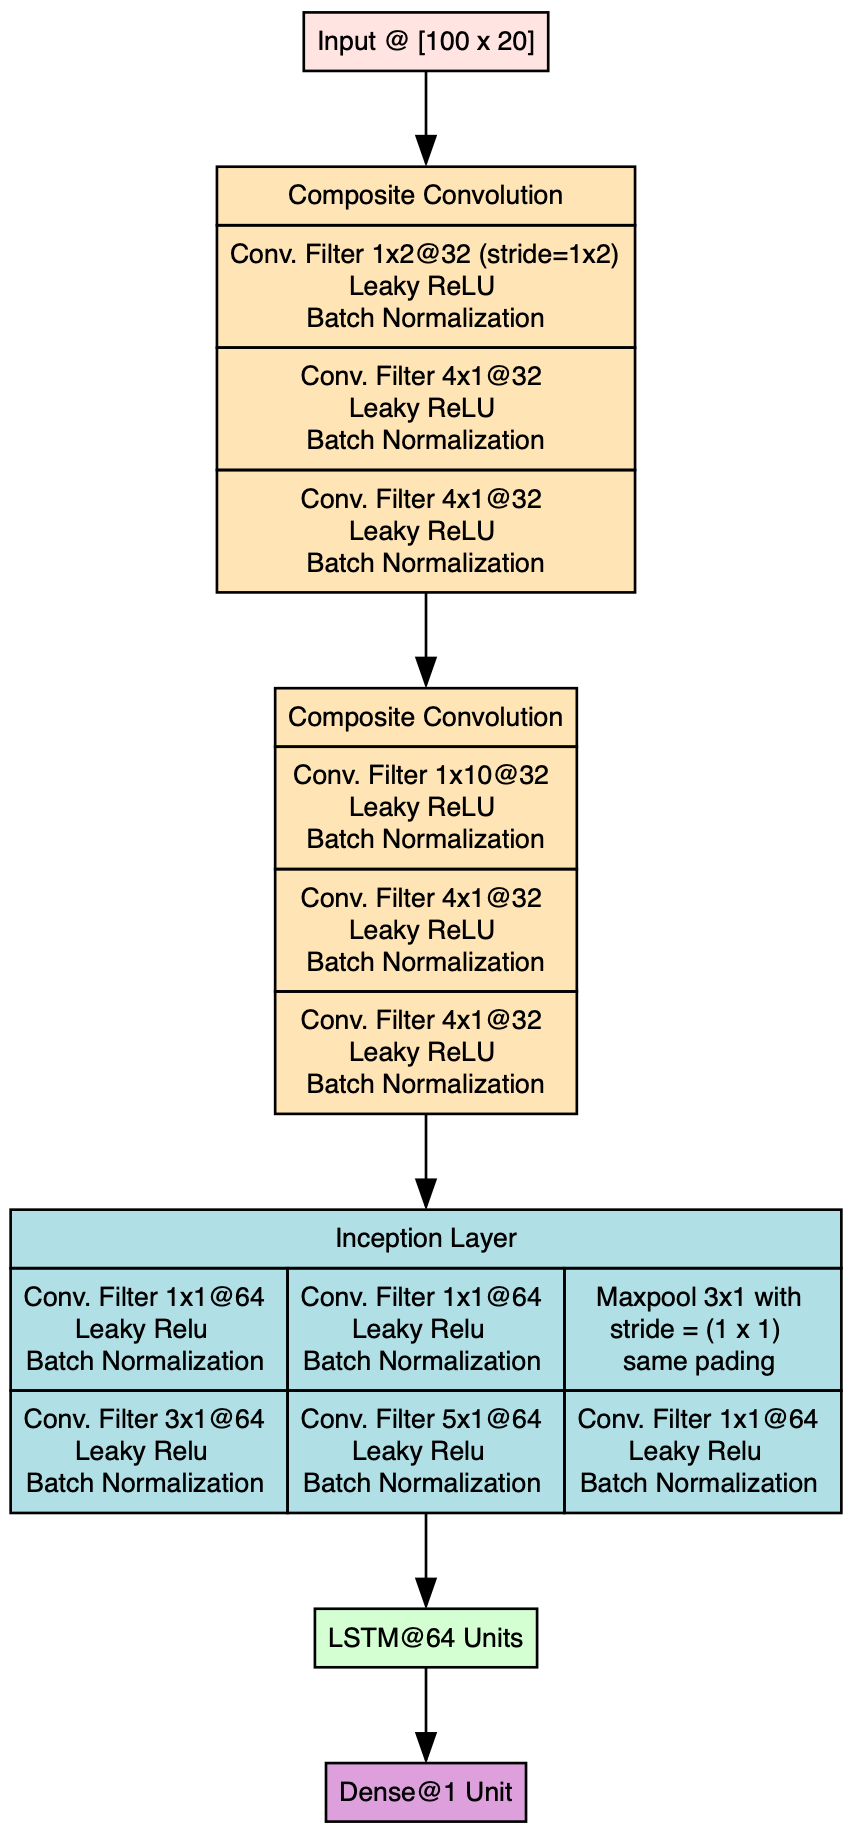
\includegraphics[height=7.5in]{cnn_lstm.png}    
    \caption{Illustration of the CNN-LSTM architecture.}
    \label{fig:cnn_lstm_architecture}
\end{figure}

\subsubsection{The DeepLOB Architecture}

Similarly, the DeepLOB architecture by Zhang et al. \cite{Zhang_2019} adds an extra composite convolutional layer at the top of the CNN-LSTM architecture and takes raw prices and volumes as inputs. Formally $\deeplob : \R^{N \times 100 \times 40} \rightarrow \R^{N \times K}$ with

$$
\deeplob(\mathbf{X}) = \fullyconnected_K \circ \lstm_{64} \circ \perm^{3, 2} \circ \mathrm{IL} \circ \mathrm{CConv}^{10}_1 \circ \mathrm{CConv}^{2, (2)}_2 \circ \mathrm{CConv}^{2, (1)}_2 (\mathbf{X}).
$$
Here, $\mathbf{X}$ is a 3D tensor of whitened limit order book price-volume information as defined in Section~\ref{SubSect:LOB-MBO}:

$$
\mathbf{X} = \left[\tilde{\mathbf{l}}^{\mathcal{P}^{(E)}}_{i_1 - 99 : i_1}, \tilde{\mathbf{l}}^{\mathcal{P}^{(E)}}_{i_2 - 99 : i_2},\dots, \tilde{\mathbf{l}}^{\mathcal{P}^{(E)}}_{i_N - 99 : i_N} \right].
$$

Table \ref{tab:deeplob} illustrates the components of this network assuming a scalar target variable ($K = 1$) and a batch of size 32 ($N = 32$). The resulting model comprises $143,777$ parameters.


% Please add the following required packages to your document preamble:
% \usepackage{booktabs}
\begin{table}[htb]
  \caption{DeepLOB architecture components.}
  \label{tab:deeplob}

\centering
\begin{tabular}{@{}lcccc@{}}
\toprule
Layer           & Notation           & Input shape        & Output shape          & Trainable Parameters  \\ \midrule
Conv. Layer     & $\mathrm{CConv}^{2, (1)}_{2}$ & $(32, 1, 100, 40)$ & $(32, 32, 94, 20)$   & 8544                  \\
Conv. Layer     & $\mathrm{CConv}^{2, (2)}_2$   & $(32, 32, 94, 20)$ & $(32,  32,  88, 10)$ & 10528                 \\
Conv. Layer     & $\mathrm{CConv}^{10}_1$       & $(32, 32, 88, 10)$ & $(32, 32, 82, 1)$    & 18720                 \\
Inception Layer & $\mathrm{IL}$               & $(32,  32, 82, 1)$ & $(32, 194, 82, 1)$   & 39872                 \\
Permutation     & $\perm^{3,2}$        & $(32, 194, 82, 1)$ & $(32, 82, 194, 1)$   & 0                     \\
LSTM            & $\lstm_{64}$        & $(32, 82, 194)$    & $(32, 64)$           & 66048                 \\ 
Fully Connected & $\fullyconnected_{1}$    & $(32, 64)$         & $(32, 1)$            & 65   \\\bottomrule
\end{tabular}

\end{table}



\clearpage
\section{Stationarity Testing}
\label{ap:stationarity_testing}

It is well known in forecasting theory that exogenous variables must be stationary to avoid spurious regressions \cite{xie2006spurious}. Three main tests are adopted:

\noindent \textbf{(A) Augmented Dickey--Fuller (ADF) Test.}
For any variable \(y\) (see Section~\ref{subsec:data_collection}), the ADF test with local trend considers the following autoregressive model:
\[
y_j 
= 
c + \bigl(1 - \phi_1 B - \phi_2 B^2 - \dots - \phi_p B^p\bigr) y_j 
+ 
\varepsilon_j,
\]
which can be equivalently written as
\begin{equation}
\Delta y_j 
= 
\alpha + \gamma y_{j - 1} 
+ 
\sum_{k = 1}^{p - 1} \zeta_k \,\Delta y_{j - k} 
+ 
\varepsilon_j,
\label{eq:adf_autoreg}
\end{equation}
where \(\rho = \sum_{\ell=1}^{p}\phi_\ell\), \(\zeta_k = -\sum_{\ell=k+1}^{p}\phi_\ell\), \(\gamma = \rho - 1\), and \(B\) is the backshift operator. Note that \(\gamma \le 0\), and \(\gamma = 0\) corresponds to \(\rho = 1\), indicating a unit root in \(\phi(z) = 1 - \phi_1 z - \dots - \phi_p z^p\). The ADF test compares
\[
H_0^{\text{ADF}}: \gamma = 0 
\quad \text{versus} \quad
H_1^{\text{ADF}}: \gamma < 0.
\]
Implementation details follow \cite{banerjee1993co} and are available in the \verb|fUnitRoots| package \cite{funitroots2024}. The test statistic is
\[
Z^{\text{ADF}}_t 
= 
\frac{\hat{\gamma}}{\text{s.e.}(\hat{\gamma})},
\]
where \(\hat{\gamma}\) is estimated by ordinary least squares (OLS) on \eqref{eq:adf_autoreg}. Because \(Z^{\text{ADF}}_t\) follows a distribution derived from stochastic integrals rather than a Student’s \(t\)-distribution, the critical values differ accordingly \cite{banerjee1993co}.

A well-known drawback of the ADF test is its sensitivity to the choice of lag length \(p\). In practice, this requires manual input or automated procedures. For simplicity, the current setup fixes \(p = 10\) for all variables. Results from the ADF test are then compared with those of the PP test, which removes the lag-length requirement at the cost of reduced power.

\noindent \textbf{(B) Phillips--Perron (PP) Test.}
The PP test uses a baseline model:
\[
y_j 
= 
\rho\,y_{j - 1} + u_j, 
\quad 
u_j 
= 
\sum_{k=0}^{\infty} \psi_k \,\varepsilon_{j - k} 
= 
\psi(B)\,\varepsilon_j,
\]
where \(\varepsilon_j\) is an iid sequence of random variables with mean zero and variance \(\sigma^2\). Assuming \(\sum_{k=0}^{\infty} k\,\psi_k < \infty\), define 
\(\gamma_k = \mathbb{E}[u_j \,u_{j-k}] = \sigma^2 \sum_{s=0}^{\infty} \psi_s \psi_{s + k}\) and 
\(\lambda = \sigma \sum_{s=0}^{\infty} \psi_s = \sigma\,\psi(1)\). The test contrasts
\[
H_0^{\text{PP}}: \rho = 1 
\quad \text{versus} \quad
H_1^{\text{PP}}: |\rho| < 1.
\]
The statistic is
\[
Z_{\tau}^{\text{PP}} 
= 
\Bigl(\frac{\hat{\gamma}_0}{\hat{\lambda}^2}\Bigr)^{\!1/2}
\frac{\hat{\rho} - 1}{\text{s.e.}(\hat{\rho})}
\;-\;
\frac{1}{2}\Bigl(\hat{\lambda}^2 - \hat{\gamma}_0\Bigr)
\Bigl(\frac{\hat{\lambda}^2}{\sum_{j=1}^{T}(y_j - \bar{y})^2}\Bigr)^{\!1/2},
\]
where 
\begin{align*}
\hat{\gamma}_k 
&= 
\frac{1}{T} \sum_{j=k+1}^{T} \hat{u}_j\,\hat{u}_{j - k},\\
\hat{\lambda}^2 
&= 
\hat{\gamma}_0 
+ 
2 \sum_{k=1}^{q} \Bigl(1 - \frac{k}{q+1}\Bigr)\,\hat{\gamma}_k,\\
q 
&= 
\Bigl\lfloor 12 \Bigl(\frac{T}{100}\Bigr)^{1/4}\Bigr\rfloor.
\end{align*}
Since \(Z_{\tau}^{\text{PP}}\) depends on functionals of Brownian motion rather than standard distributions, critical values must be derived from the appropriate asymptotic theory. This test is implemented via the \verb|urca| package \cite{urca}.

\noindent \textbf{(C) KPSS Test.}
For completeness, the Kwiatkowski--Phillips--Schmidt--Shin (KPSS) test \cite{kwiatkowski1992testing} is included in a confirmatory role. Unlike the ADF and PP tests, the KPSS null hypothesis assumes stationarity. The model is
\[
y_j 
= 
r_j + u_j,
\quad
r_j 
= 
r_{j - 1} + e_j,
\]
where \(e_j\) is an iid sequence with zero mean and variance \(\sigma^2_e\), and \(u_j\) satisfies properties similar to those in the PP framework. That is $u_j = \psi(B) \varepsilon_j$, for some $\varepsilon \overset{iid}{\thicksim} (0, \sigma^2)$, and $\sum^{\infty}_{k = 0} k \psi_k < \infty$. The hypotheses are
\[
H^{KPSS}_0: \sigma_{e}^2 = 0 
\quad\text{versus}\quad 
H^{KPSS}_1: \sigma_{e}^2 > 0.
\]
The test statistic is
\[
\hat{\eta}_{\mu}^{\text{KPSS}} 
= 
\sum_{k=1}^{T} 
\frac{S_k^2}{\hat{\lambda}^2},
\]
where \(S_k = \sum_{j=1}^{k} \hat{u}_j\) represents the partial sum of residuals 
(\(\hat{u}_j = y_j - \bar{y}\)), and \(\hat{\lambda}^2\) follows the same form as in the PP test. As in the previous tests, critical values derive from nonstandard limiting distributions. The \verb|urca| package used for computing the rejection region of the this test.

\clearpage
\section{Case Study: Model Subspace Selection}
\label{ap:case_study_var_selection}

This Monte Carlo study compares adaptive LASSO (adaLASSO) \citep{Zou01122006,MEDEIROS2016255} with OLS-Bonferroni selection for exact support recovery and examines how quickly the failure probability decays to zero. The study is organized as follows. Section~\ref{subsec:background} reviews the Medeiros~\&~Mendes framework describing the DGP and assumptions presented in \cite{MEDEIROS2016255}.  Section~\ref{subsec:simulation_design} describes the particular DGP used for the simulations and the dynamics of design space growth. Section~\ref{subsec:results_and_discussion} analyzes the simulated data to quantify the effect of multicollinearity and initial weights selection. Section~\ref{subsec:conclusions_and_recommendations} draws conclusions and recommendations and Section~\ref{subsec:reproducibility} provides precise instructions for the replication of the present study.

\subsection{Background}
\label{subsec:background}

This section discusses the key regularity conditions and results in \cite{MEDEIROS2016255} and provides some intuitive interpretation to these ideas.

First, consider the data generating process (DGP) 

\begin{equation}
    y_t = \alpha_0 + \boldsymbol{\theta}^T\,\mathbf{x}_t + u_t.
    \label{eq:dgp_medmen}
\end{equation}
Here, $\{\mathbf{x}_t\}_{t \in \Z}$ is an $n_T$-dimensional covariate process, which possibly contains lags of the endogenous process, and $\{u_t\}_{t \in \Z}$ is a martingale difference sequence. Denote by $T$ the sample size of observations of the process $\{y_t \}_{t\in \Z}$, $n_T$ the total number of covariates, and $s_T$ the number of relevant covariates. For simplicity assume that the first $s_T$ elements of $\mathbf{x}_t$ correspond to the relevant variables, which can effectively be denoted as $\mathbf{x}_t = [\mathbf{x}_t(1), \mathbf{x}_t(2)]$. Also write $\boldsymbol{\theta}^T = [\boldsymbol{\theta}^T(1), \boldsymbol{\theta}^T(2)]$ and let $\boldsymbol{\theta}_0$ denote the true parameter which effectively implies that $\boldsymbol{\theta}_0^T = [\boldsymbol{\theta}_0^T(1), \mathbf{0}^T]$. Assuming, without loss of generality, that $\alpha_0 = 0$, The adaLASSO technique consists in minimizing the objective function given by

\[
        f(\boldsymbol{\theta}) = \bigl\|\mathbf{y} -  \mathbf{X}\boldsymbol{\theta}\bigr\|_2^2
        \;+\;\lambda_T\sum_{k} w_k\,|\theta_k|.
\]
Here, $w_k = \left| \theta_{I, k} \right|^{-\tau}$ are computed from $\tau > 0$ and $\boldsymbol{\theta}_I$ an initial parameter estimate. The initial parameter estimate could be given, among others, by OLS, LASSO or elastic-net. The choice of the algorithm for the initial parameters is left out of the scope of this simulation study. Medeiros and Mendes group their assumptions into four categories: Data Generating Process (DGP), Design Space (DESIGN), Initial Weights (WEIGHTS), and Regularization Parameter (REG). These assumptions are restated below for self-completeness.


\begin{itemize}
  \item[(DGP1)] Define $\mathbf{Z}_t = (\mathbf{x}_t^T,\,u_t)^T$. $\{\mathbf{Z}_t\}_{t \in \Z}$ is zero–mean and weakly stationary.
  \item[(DGP2)] $\E \left\{ u_t\mid \SigAl_t\right\}=0$, where $\SigAl_t=\sigma(\mathbf{x}_t, \mathbf{Z}_{t-1}, \mathbf{Z}_{t-2},\dots)$.
  \item[(DGP3)] 
  \[
     \max_{1\le i\le n_T}\Bigl|\tfrac1T\sum_{t=1}^T(x_{it}^2 - E[x_{it}^2])\Bigr|\;\xrightarrow[]{\Prob}0.
  \]
  \item[(DGP4)] For some $m \geq 2$, there exists $c_m < \infty$ such that
  
  \[
     \E\bigl|x_{it}\,u_t\bigr|^m\;\le c_m \quad \forall t\in \Z, i \in1:n_T.
  \]

  \item[(DESIGN1)] The true parameter $\boldsymbol{\theta}_0$ belongs to an open subset $\boldsymbol{\Theta}_{n_T} \subseteq \mathbb{R}^{n_T}$ that contains the origin.
  \item[(DESIGN2)] There exists $\theta_{\min} > 0$ such that $\min_{i\le s_T}|\theta_{0,i}|>\theta_{\min}$.
  \item[(DESIGN3)] Denote $\hat{\boldsymbol{\Omega}}_{11} := \frac{1}{T}\mathbf{X}^T(1) \mathbf{X}(1)$ and $\boldsymbol{\Omega}_{11} := \E \left\{ \mathbf{x}_t(1) \mathbf{x}^T_t(1) \right\}$
    \begin{enumerate}
      \item[(a)] There exists a constant $\phi_{\min} \in (0, 1)$ such that
      $$
      \inf_{\norma{\boldsymbol{\alpha}} = 1} \boldsymbol{\alpha}^T \boldsymbol{\Omega}_{11} \boldsymbol{\alpha} > 2 \phi_{\min}.
      $$
      Note that this is equivalent to the smallest eigenvalue of $\boldsymbol{\Omega}_{11}$ being greater than $2\phi_{\min}$.
      \item[(b)] $\norma{\boldsymbol{\Omega}_{11} - \hat{\boldsymbol{\Omega}}_{11}}_{\infty} = \max_{ij} \left| \boldsymbol{\Omega}_{11} - \hat{\boldsymbol{\Omega}}_{11}\right|_{ij} \leq \frac{\phi_{\min}}{s_T}$
      
    \end{enumerate}

  \item[(WEIGHTS1)] The weights on inactive endogenous variables diverge fast enough: for some $\xi\in(0,1)$ and $c_w>0$,
  \[
    \min_{i \in s_T + 1 : n_T} T^{-\xi/2}\,w_i \;>\; c_w\,\sqrt{\frac{s_T}{\phi_{\min}}},
  \]
  with probability converging to one
  \item[(WEIGHTS2)] The weights on the active set are uniformly bounded: 
  \[
     \sum_{i=1}^{s_T} w_i^2 < s_T \,w_{\max, T}^2,\quad w_{\max, T}<T^{\xi/2},
  \]
  with probability converging to one.
\end{itemize}

\begin{itemize}
    \item[(REG)] Let $\lambda_T>0$ be the Adaptive‐LASSO penalty parameter.  It is required that
\[
   \frac{n_T^{1/m}T^{(1-\xi)/2}}{\lambda_T}\;\xrightarrow[T \to \infty]{} 0
   \quad\text{and}\quad
   \frac{\lambda_T}{\sqrt{T}}\,\frac{s_T^{1/2}}{w_{\max, T}\,\phi_{\min}}\; \xrightarrow[T \to \infty]{} 0.
\]
\end{itemize}

Further examination of these assumptions reveal interesting patterns. For analysis convenience, define the following dynamics

\begin{align*}
n_T &= \lceil c_{\delta}\,T^{\delta} \rceil, \\[6pt]
s_T &= \lceil c_{\gamma}\,T^{\gamma} \rceil, \\[6pt]
\lambda_T &= c_{\alpha} n_T^{1/m}\;T^{\frac{1-\xi}{2} + \frac{\alpha}{m}}, \\[6pt]
w_{S,T}^2 &= c_{\beta_S}\,T^{\beta_S}, 
\quad
w_{S^c,T}^2 = c_{\beta_{S^c}}\,T^{\beta_{S^c}}.
\\[4pt]
\end{align*}
Here, $w_{S,T}$ and $w_{S^c,T}$ model the growth order of the active and inactive weights respectively. Basic calculus shows that the assumptions (WEIGHTS1), (WEIGHTS2), and (REG) above can be rewritten as

\begin{align*}
\beta_{S^c} - \xi &> \gamma, 
  &&\text{(WEIGHTS1)}\\
\beta_S &< \xi, 
  &&\text{(WEIGHTS2)}\\
\alpha > 0,\quad 
\frac{2}{m}\bigl(\alpha + \delta\bigr) &< \xi - \gamma - \beta_S. 
  &&\text{(REG)}
\end{align*}
These inequalities reveal interesting relationships under the light of the following results.

\begin{theorem}[Theorem 1 of \cite{MEDEIROS2016255}] Under Assumptions \textup{DGP}, \textup{DESIGN}, \textup{WEIGHTS} and \textup{REG}, suppose moreover that
\[
\theta_{\min}
>
\frac{\lambda_T\,s_T^{1/2}}{
  T^{1-\xi/2}\,\phi_{\min}
}.
\]
Then the adaptive LASSO estimator $\hat\theta$ satisfies
\[
\Prob\bigl(\mathrm{sign}(\hat\theta)=\mathrm{sign}(\theta_0)\bigr)
\;\xrightarrow[T \rightarrow \infty]{} 1.
\]
\label{thm:1_medeiros}
\end{theorem}

In the theorem above, the $\mathrm{sign}$ function is defined as $\mathrm{sign}(x) = I_{\{ x > 0 \}} - I_{\{ x < 0 \}}$ which implies that $\mathrm{sign}(0) = 0$.

\begin{theorem}[Theorem 2 of \cite{MEDEIROS2016255}] Let $\hat{\boldsymbol{\theta}}_{\text{ols}}{(1)}$ denote the OLS estimator of the true active coefficients $\boldsymbol{\theta}_0{(1)}$.  Under the assumptions of Theorem~\ref{thm:1_medeiros}, it holds that for any $s_T$‑vector $\boldsymbol{\alpha}$ with $\|\boldsymbol{\alpha}\|_2=1$,
\[
\sqrt{T}\,\boldsymbol{\alpha}^T\,\bigl(\hat{\boldsymbol{\theta}}{(1)} - \boldsymbol{\theta}_0{(1)}\bigr)
=
\sqrt{T}\,\boldsymbol{\alpha}^T\,\bigl(\hat{\boldsymbol{\theta}}_{\text{ols}}{(1)} - \boldsymbol{\theta}_0{(1)}\bigr)
\;+\;o_p(1).
\]
\end{theorem}

Theorem 2—often called the \textit{oracle property}—goes one step further: not only does the adaptive LASSO select the correct support with probability tending to one, but its active‐set estimates are asymptotically as efficient as if we knew the true model in advance. Moreover, the proof of Theorem 1 shows that, for some $c>0$ and for a sufficiently large \(T\),
\begin{equation}
\Prob\bigl(\mathrm{sign}(\hat\theta)\neq\mathrm{sign}(\theta_0)\bigr)
\;\le\;
\frac{c}{T^\alpha},
\label{eq:decay_rate}
\end{equation}
so the probability of selection failure decays at rate \(T^{-\alpha}\). In practice this means that larger \(\alpha\) yields faster convergence—yet \(\alpha\) itself is bounded by the REG assumption’s \textit{window}. Note also that heavier‐tailed errors (smaller \(m\)) tighten this window, as do steeper growth in the number of covariates, denser true parameter vectors \(\theta_0\), or more aggressive penalization on the active set.

\subsection{Simulation Design}
\label{subsec:simulation_design}


Simulated data is generated from the DGP

\begin{equation*}
y_t 
= 
\displaystyle \phi y_{t - 1}
\;+\;
\sum^{n_T}_{j = 1} \beta_j\,x_{j t}
\;+\; u_t,  
\end{equation*}
where,

\[
\begin{cases}
\mathbf{x}_t=
\displaystyle \phi_X \,\mathbf{x}_{t-1}
\;+\;
\mathbf{L}\,\mathbf{v}_t,
&
v_{jt} \overset{iid}{\sim} t_{m + 1},\\[2ex]
u_t = \sigma_t \eta_t 
&
\eta_t \overset{iid}{\sim} t_{m + 1},\\[2ex]
\sigma^2_t = \omega + \alpha_{\star} u_{t - 1}^2 + \beta_{\star} \sigma^2_{t - 1}.
\end{cases}.
\]
Here, $\phi_X$ is a scalar and $\mathbf{L}$ is chosen to be a lower triangular matrix such that $\mathbf{R} := \mathbf{L} \mathbf{L^T}$, where $\mathbf{R}$ is the desired correlation matrix. Take $\beta_j = 1$ if $j \leq s_T$ and zero otherwise. Take $\phi = 0.8$, $\phi_X = 0.5$, $\omega = 0.1$, $\alpha_\star = 0.1$, $\beta_\star = 0.8$, and $m = 8$. Construct $\mathbf{R}$ starting from the identity matrix and replace its entries $(1, 2)$ and $(2, 1)$ with $\rho$ (i.e. $\mathbf{R}_{1,2} = \mathbf{R}_{2,1} = \rho$), where $\rho \in \{0, 0.25, 0.5, 0.75, 0.99 \}$. The parameters governing the dynamics of the number of candidate variables and penalizing weights are given below.


\begin{table}[h]
  \caption{Simulation parameters.}

\centering
\begin{tabular}{ccccccccccc}
\hline
$c_{\alpha}$ & $\alpha$ & $c_{\beta_{S}}$ & $\beta_{S}$ & $c_{\beta_{S^c}}$ & $\beta_{S^c}$ & $c_{\gamma}$ & $\gamma$ & $c_{\delta}$ & $\delta$ & $\xi$ \\
\hline
1 & 0.25 & 1 & 0.125 & 1 & 1.5 & 2 & 0.25 & 1 & 0.5 & 0.75 \\
\hline
\end{tabular}

\end{table}

Partitioning the interval $[64,1024]$ into 15 roughly equally‐spaced values of $T$ produces the simulation grid shown in Table~\ref{tab:simulation_grid}.  Each $(T,n_T,s_T)$ configuration is then replicated $N=100$ times for each of the specified correlation levels. For each of the samples, adaLASSO is fit assuming equal weights for the active set ($w_{S,T}$) and weights equal to $w_{S^c, T}$ for the inactive set. This helps to control the dynamics of the penalizing weights which in practice emerge from $\tau$ and the initial estimate selection algorithm. For simplicity, the weight corresponding to the lagged value of $y_t$ is left close to zero and only one lag is included in $\mathbf{X}$. OLS is then fit and the variance of $\hat{\tilde{\boldsymbol{\beta}}}$ is estimated via the homoskedastic formula (as a benchmark) and the heteroskedasticity-consistent estimator (HCE). Specifically

\begin{align*}
    \hat{V}_{\mathrm{hom}} &= \hat{\sigma}^2(\tilde{\boldsymbol{X}}^T \tilde{\boldsymbol{X}})^{-1}; \quad  \hat{\sigma}^2 = \frac{1}{T - n_T - 1}\sum^{T}_{t = 1} \hat{u}_t^2,\\
    \hat{V}_{\mathrm{het}} &= (\tilde{\boldsymbol{X}}^T \tilde{\boldsymbol{X}})^{-1} \left( \sum^T_{t = 1} \tilde{\mathbf{x}}_t \tilde{\mathbf{x}}^T_t \hat{u}^2_t \right) (\tilde{\boldsymbol{X}}^T \tilde{\boldsymbol{X}})^{-1},
\end{align*}
where in the above the \textit{tilded} quantities denote the corresponding augmented quantity to account for the inclusion of one lag of the endogenous variable. Statistical significance is assessed throught the $t$ test with Bonferroni correction. That is, a variable will be selected following each of the OLS approaches iff

\begin{align*}
    \frac{\hat{\tilde{\beta}}_i}{V_{ii}^{1 / 2}} > t_{T - s_T - 1, 1 - \frac{0.025}{(n_T + 1)}}.
\end{align*}
Following the execution of these three variable selection algorithms. The proportion of correctly selected models is calculated for each of the different $T \rho$-combinations.


\begin{table}[ht]
  \caption{Simulation grid: sample size $T$ and corresponding $n_{T}=\lceil c_{\delta} T^{\delta}\rceil$, $s_{T}=\lceil c_{\gamma}T^{\gamma}\rceil$.}
  \label{tab:simulation_grid}

\centering
\begin{tabular}{ccc}
\toprule
$T$   & $n_{T}$ & $s_{T}$ \\
\midrule
64    &  8  &  6  \\
133   & 12  &  7  \\
202   & 15  &  8  \\
270   & 17  &  9  \\
339   & 19  &  9  \\
407   & 21  &  9  \\
476   & 22  & 10  \\
544   & 24  & 10  \\
613   & 25  & 10  \\
682   & 27  & 11  \\
750   & 28  & 11  \\
819   & 29  & 11  \\
887   & 30  & 11  \\
956   & 31  & 12  \\
1024  & 32  & 12  \\
\bottomrule
\end{tabular}

\end{table}




\subsection{Results and Discussion}
\label{subsec:results_and_discussion}

\subsubsection{Multicollinearity Effect}

Figure~\ref{fig:exact_recovery_corr} (see Section \ref{sec:comp_tables_figs}) displays the exact recovery rate (fraction of simulations where $\mathrm{sign}(\hat{\boldsymbol{\theta}}) = \mathrm{sign}(\boldsymbol{\theta})$) as a function of $T$, for different correlation levels $\rho$. Several clear patterns emerge. First, as expected, increasing the sample size improves support recovery for both methods in all scenarios – the curves generally rise toward 1.0 as $T$ grows. However, the adaLASSO (red curves) achieves much higher recovery rates at moderate sample sizes than OLS (blue/green curves) in the presence of strong multicollinearity. For low correlation ($\rho=0$ or $0.25$), the gap between methods is small: OLS with Bonferroni performs nearly as well as adaLASSO when predictors are independent or only mildly correlated. In fact, for $\rho=0$, both methods eventually reach ~100\% recovery with sufficiently large $T$ (hundreds of observations), and their trajectories are quite close. This is because when predictors are uncorrelated, the OLS t-tests remain informative (each coefficient can be estimated independently with little variance inflation), so the Bonferroni penalty for multiple testing is the main hurdle – which large $T$ can overcome by reducing standard error. AdaLASSO also works well in this regime, effectively similar to the ordinary LASSO which is known to be consistent under mutual independence of features.

When correlation increases to moderate levels ($\rho=0.5$ shown in Figure \ref{fig:exact_recovery_corr}, top-right panel, and $\rho=0.75$ in bottom-left), the performance of OLS selection deteriorates dramatically relative to adaLASSO. For $\rho=0.5$, the OLS method (blue/green lines) requires a much larger $T$ to approach high recovery probability – there is a noticeable rightward shift of the OLS curve compared to the adaLASSO curve. The adaLASSO achieves near-perfect support recovery at $T = 339$ observations when $\rho=0.5$, whereas OLS-Bonferroni needs roughly double that sample size to reach comparable accuracy. The gap widens further at $\rho=0.75$: here the OLS approach almost never succeeds for small or moderate samples (recovery probability essentially 0 for $T < 300$). Even at $T = 1024$, OLS is only recovering the true model in about 50–60\% of trials, whereas adaLASSO already exceeds 90\% success by that point.  the adaLASSO appears more robust to multicollinearity when $T$ is large enough, eventually achieving near-certain recovery even at $\rho=0.75$ in the simulations (red curve tending to 1.0 as $T$ grows). OLS, however, remains very sensitive: even at $T=1024$, the OLS method never reaches 100\% recovery for $\rho=0.75$.

The most extreme case is $\rho=0.99$ (Figure~\ref{fig:exact_recovery_corr}, bottom-middle), where predictors are almost perfectly correlated. This scenario is akin to having duplicate or nearly-duplicate variables in the dataset – a problem for OLS inference. Accordingly, the OLS selection method essentially fails entirely: the blue/green curves at $\rho=0.99$ sit near zero across all sample sizes tested. The adaLASSO (red curve) also finds this scenario challenging (its recovery probability grows only slowly with $T$ and does not reach 1 even at $T = 1024$), but it clearly outperforms OLS: by $T = 1024$ observations, adaLASSO achieves about 70\% exact recovery, whereas OLS is essentially at 0\%. This sensitivity to multicollinearity of the adaLASSO approach connects with the assumption DESIGN3 as $\phi_{\mathrm{min}}$ decreases with $\rho$. The simulation confirms that multicollinearity breaks down the performance of naive OLS variable selection, while adaLASSO is far more resilient in discovering the correct predictors (especially as $T$ becomes large).

To connect with the theoretical result from \cite{MEDEIROS2016255} (see \ref{eq:decay_rate}), the rate at which the failure probability decreases with $T$ is examined. Figure~\ref{fig:log_log_failure_rate_corr} plots the Monte Carlo estimated failure rates on logarithmic scales. If the failure probability follows a power-law $T^{-\alpha}$, an approximately straight line with slope $-\alpha$ in the log–log representation would be observed. Indeed, for the adaLASSO (red) a roughly linear downward trend in all panels is seen - except when the curve saturates -, consistent with a polynomial decay in $T$. At every correlation level, the estimated failure rate (red) declines faster than the theoretical bound line (dashed), indicating a steeper power‑law exponent. Thus, the adaLASSO simulation results are consistent with the theoretical guarantee of polynomial-decay consistency: even under dependence and heavy-tailed noise, it is observed that $\Prob\bigl(\mathrm{sign}(\hat\theta)\neq\mathrm{sign}(\theta_0)\bigr)$ trends down at least as fast as $c T^{-\alpha}$ for some $\alpha>0$.

The OLS-based methods (blue/green lines in Figure \ref{fig:log_log_failure_rate_corr}) tell a similar story when the multicollinearity level is below or at 50\%. However, the failure probability rate of decrease exhibits a slower convergence when the multicollinearity level is at or above 75\%. This reflects the fact that OLS with Bonferroni can eventually consistently select the true model when predictors have low to moderate correlation. For higher correlations ($\rho \geq 0.75$), the blue/green points in Figure \ref{fig:log_log_failure_rate_corr} are almost horizontal or very mildly declining on the log–log scale. This underscores the superior performance of adaLASSO under high multicollinearity regimes when the DGP, DESIGN, WEIGHTS, and REG conditions hold.

\subsubsection{Effect of Initial Weights}

It might be suggested that adaLASSO may enjoy an unfair edge under the simulation configuration presented, since the true parameter values are “encoded” in the evolution of the penalty weights \(w_i\). To address this concern, a targeted sensitivity experiment was conducted: setting the correlation parameter \(\rho=0\) and raising the inactive‐set weights to \(\beta_{S^c}=1.15\), while holding all other hyper‐parameters fixed. The results (Figures~\ref{fig:exact_recovery_beta} and~\ref{fig:log_log_failure_rate_beta}) show that, under these conditions, adaptive‐LASSO requires substantially larger sample sizes before its exact‐recovery probability saturates. Crucially, however, once the sample size exceeds a threshold, the failure probability decays very rapidly, in line with the oracle‐type behavior predicted by theory.

These findings make clear that careful tuning of the initial‐weight construction is important when \(T\) is limited or the signal in the inactive set is relatively strong.

\subsection{Conclusions and Recommendations}
\label{subsec:conclusions_and_recommendations}

In this Monte Carlo case study the adaLASSO and Bonferroni-corrected t-tests were compared, focusing on exact support recovery and the empirical rate at which the failure probability decays to zero.  The main findings are:

\begin{itemize}
  \item \textbf{Exact recovery vs.\ multicollinearity.}  When predictors are uncorrelated or only mildly correlated ($\rho\le0.25$), both methods eventually recover the true support with high probability as $T$ grows.  However, under moderate to strong multicollinearity ($\rho\ge0.5$), OLS-Bonferroni requires much larger $T$ and in extreme cases ($\rho=0.99$) essentially fails, whereas adaLASSO still achieves a decent recovery rate for moderately large samples.
  \item \textbf{Polynomial decay of failure rate.}  On a log–log scale, the adaLASSO’s failure probability exhibits an approximately linear decline of slope $-\alpha$, consistent with the theoretical bound
  \[
    \Pr\bigl(\mathrm{sign}(\hat\theta)\neq\mathrm{sign}(\theta_0)\bigr)\;\lesssim\;c\,T^{-\alpha}.
  \]
  In contrast, OLS-Bonferroni only attains an adaLASSO-comparable decay when $\rho$ is small; its curve flattens out for higher correlations.
  \item \textbf{Sensitivity to initial‐weight tuning.}  By increasing the inactive‐set exponent $\beta_{S^c}$, it was shown that adaLASSO may require larger $T$ before its recovery probability ``saturates.''  Yet once past a moderate threshold, its convergence is very rapid, demonstrating the oracle‐property in practice. This underscores the importance of the selection of an initial weights selection method that discriminates inactive variables.
\end{itemize}

\noindent
\textbf{Practical recommendations.}  Based on these results, practitioners should:
\begin{itemize}
  \item Employ adaLASSO in high‐dimensional, time‐series settings where multicollinearity is present, since it substantially outperforms OLS‐based selection under dependence.
  \item Carefully tune the hyperparameters of the initial weights selection.
  \item Use OLS-Bonferroni as a simple baseline when predictors are mildly correlated.
  \item Validate selection performance before deploying the method in empirical applications.
\end{itemize}

\noindent
Overall, the present study confirms that adaLASSO not only achieves model selection consistency and the oracle property under the Medeiros \& Mendes framework, but also delivers robust performance in finite samples—especially when multicollinearity and heteroskedastic, heavy‐tailed errors are present.

\subsection{Reproducibility}
\label{subsec:reproducibility}

All the simulation results presented here can be reproduced using the code available in the GitHub repository \url{judmejiabe/case-study-adaLASSO}. The repository contains detailed scripts for generating the data, running the adaptive LASSO and OLS selection procedures, and producing the figures.

\clearpage
\section{Events Matching Exclusion Criteria on the INTC MBO Dataset}
\label{sec:exclusion_criteria}

This section lists the dates excluded from the analysis as a consequence of meeting any of the excluding criteria highlighted in Section~\ref{subsec:dataset}. The exclusion criteria is reproduced below for the reader's convenience.

\begin{itemize}
    \item Corporate actions: Ex-dividend dates, stock splits or reverse splits, share buybacks and rights issues, spin-offs, mergers, or acquisitions
    \item Earnings and company-specific news: Quarterly earnings announcements and guidance revisions, joint ventures, large partnerships or asset sales, regulatory actions or class-action lawsuits, product launches or major technological disclosures
    \item Derivative market events: Monthly options expirations (OPEX), quarterly triple witching weeks (stock index futures, index options, and single-stock options expiry), index futures rollovers (e.g., NASDAQ-100, S\&P 500), index and ETF quarterly rebalancing
    \item Scheduled announcements: U.S. Employment Situation (non-farm payrolls), Consumer Price Index (CPI), Producer Price Index (PPI), PCE releases, FOMC interest rate decisions and press conferences, other major macroeconomic indicators (e.g., GDP, JOLTS)
    \item Exchange halts: Limit-Up/Limit-Down (LULD) volatility pauses, market-wide circuit breakers, exchange-initiated suspensions (technical or regulatory).
\end{itemize}

\subsection{Corporate Actions}

\begin{itemize}
    \item May 6, 2024. Event Type: Ex-dividend date. Description: Ex-dividend date for quarterly cash dividend of \$0.125 per share. Source: \url{https://stocklytics.com/stocks/intc/dividends}
\end{itemize}

\subsection{Earnings and Company-Specific News}

\begin{itemize}
    \item April 25, 2024 (after market close, impacting May 1). Event Type: Earnings release. Description: Intel reported Q1 2024 earnings, the first quarter under its internal foundry reporting model; the Foundry segment revenue was \$4.4 billion (down 10\% year-over-year). Source: \url{https://www.intc.com/news-events/press-releases/detail/1635/intel-reports-first-quarter-2024-financial-results}
    \item May 8, 2024. Event Type: Regulatory action (export license revocation). Description: The U.S. Commerce Department revoked certain export licenses for shipments to Huawei, affecting Intel's ability to supply that customer. Source: \url{https://www.marketwatch.com/story/intels-stock-drops-after-u-s-revokes-licenses-for-exports-to-china-customer-f057da21}
    \item June 4, 2024. Event Type: Joint venture. Description: Intel and Apollo announced a definitive agreement under which Apollo acquired a 49\% equity stake in a joint venture related to Intel's Fab 34 facility in Leixlip, Ireland (Intel retains operational control). Source: \url{https://newsroom.intel.com/corporate/co-invest-program-news-2024}
    \item June 17, 2024. Event Type: Class action lawsuit. Description: Bronstein, Gewirtz \& Grossman announced a securities-fraud class action against Intel regarding statements about the internal foundry model and foundry losses (class period Jan 25--Apr 25, 2024). Source: \url{https://www.globenewswire.com/de/news-release/2024/05/13/2880132/0/en/INTC-INVESTOR-ALERT-Bronstein-Gewirtz-Grossman-LLC-Announces-that-Intel-Corporation-Investors-with-Substantial-Losses-Have-Opportunity-to-Lead-Class-Action-Lawsuit.html}
    \item June 21, 2024. Event Type: Class action lawsuit notice. Description: Levi \& Korsinsky announced a class action filing and lead-plaintiff deadline of July 2, 2024, reiterating allegations concerning Intel's internal foundry disclosures. Source: \url{https://www.prnewswire.com/news-releases/class-action-filed-against-intel-corporation-intc---july-2-2024-deadline-to-join--contact-levi--korsinsky-302178578.html}
\end{itemize}

\subsection{Derivative Market Events}

\begin{itemize}
    \item May 17, 2024. Event Type: Options expiration (OPEX). Description: Monthly U.S. equity and ETF options expiration. Source: \url{https://www.macroption.com/options-expiration-calendar/}
    \item June 17-21, 2024. Event Type: Triple witching week. Description: Simultaneous expiration of stock index futures, stock index options, and single-stock options, coinciding with June OPEX. Source: \url{https://www.bankrate.com/investing/triple-witching/}
\end{itemize}

\subsection{Scheduled Announcements}

\begin{itemize}
    \item May 3, 2024. Event Type: U.S. Employment Situation (April NFP). Description: BLS reported non-farm payrolls at 175k (below consensus), released at 8:30a ET. Source: \url{https://www.bls.gov/news.release/archives/empsit_05032024.htm}
    \item May 15, 2024. Event Type: CPI release (April). Description: Consumer Price Index data released at 8:30a ET. Source: \url{https://www.bls.gov/news.release/archives/cpi_05152024.htm}
    \item June 4, 2024. Event Type: JOLTS (Job Openings). Description: The Bureau of Labor Statistics released the April Job Openings and Labor Turnover Survey at 10:00 a.m. ET. Source: \url{https://www.bls.gov/news.release/archives/jolts_06042024.htm}
    \item June 7, 2024. Event Type: U.S. Employment Situation (May NFP). Description: Non-farm payrolls release at 8:30a ET. Source: \url{https://www.bls.gov/news.release/archives/empsit_06072024.htm}
    \item June 12, 2024. Event Type: CPI release (May). Description: Consumer Price Index release at 8:30a ET. Source: \url{https://www.bls.gov/news.release/archives/cpi_06122024.htm}
    \item June 12, 2024. Event Type: FOMC decision. Description: Federal Reserve announced policy decision and released updated Summary of Economic Projections at 2:00p ET, followed by press conference. Source: \url{https://www.federalreserve.gov/monetarypolicy/fomccalendars.htm}
    \item June 13, 2024. Event Type: PPI release (May). Description: Producer Price Index release at 8:30a ET. Source: \url{https://www.bls.gov/news.release/archives/ppi_06132024.htm}
    \item June 14, 2024. Event Type: Import/Export Prices (May). Description: BLS Import and Export Price Indexes released at 8:30a ET. Source: \url{https://www.bls.gov/news.release/archives/ximpim_06142024.htm}
\end{itemize}

\subsection{Exchange Halts}

\begin{itemize}
    \item None. No Nasdaq trading halts were recorded for INTC between May 1 and June 30, 2024. Source: Nasdaq Trader Trading Halts database \url{https://www.nasdaqtrader.com/Trader.aspx?id=TradeHalts}
\end{itemize}

\clearpage
\section{Complimentary Tables and Figures}
\label{sec:comp_tables_figs}

\begin{sidewaysfigure}[htb]
    \centering
    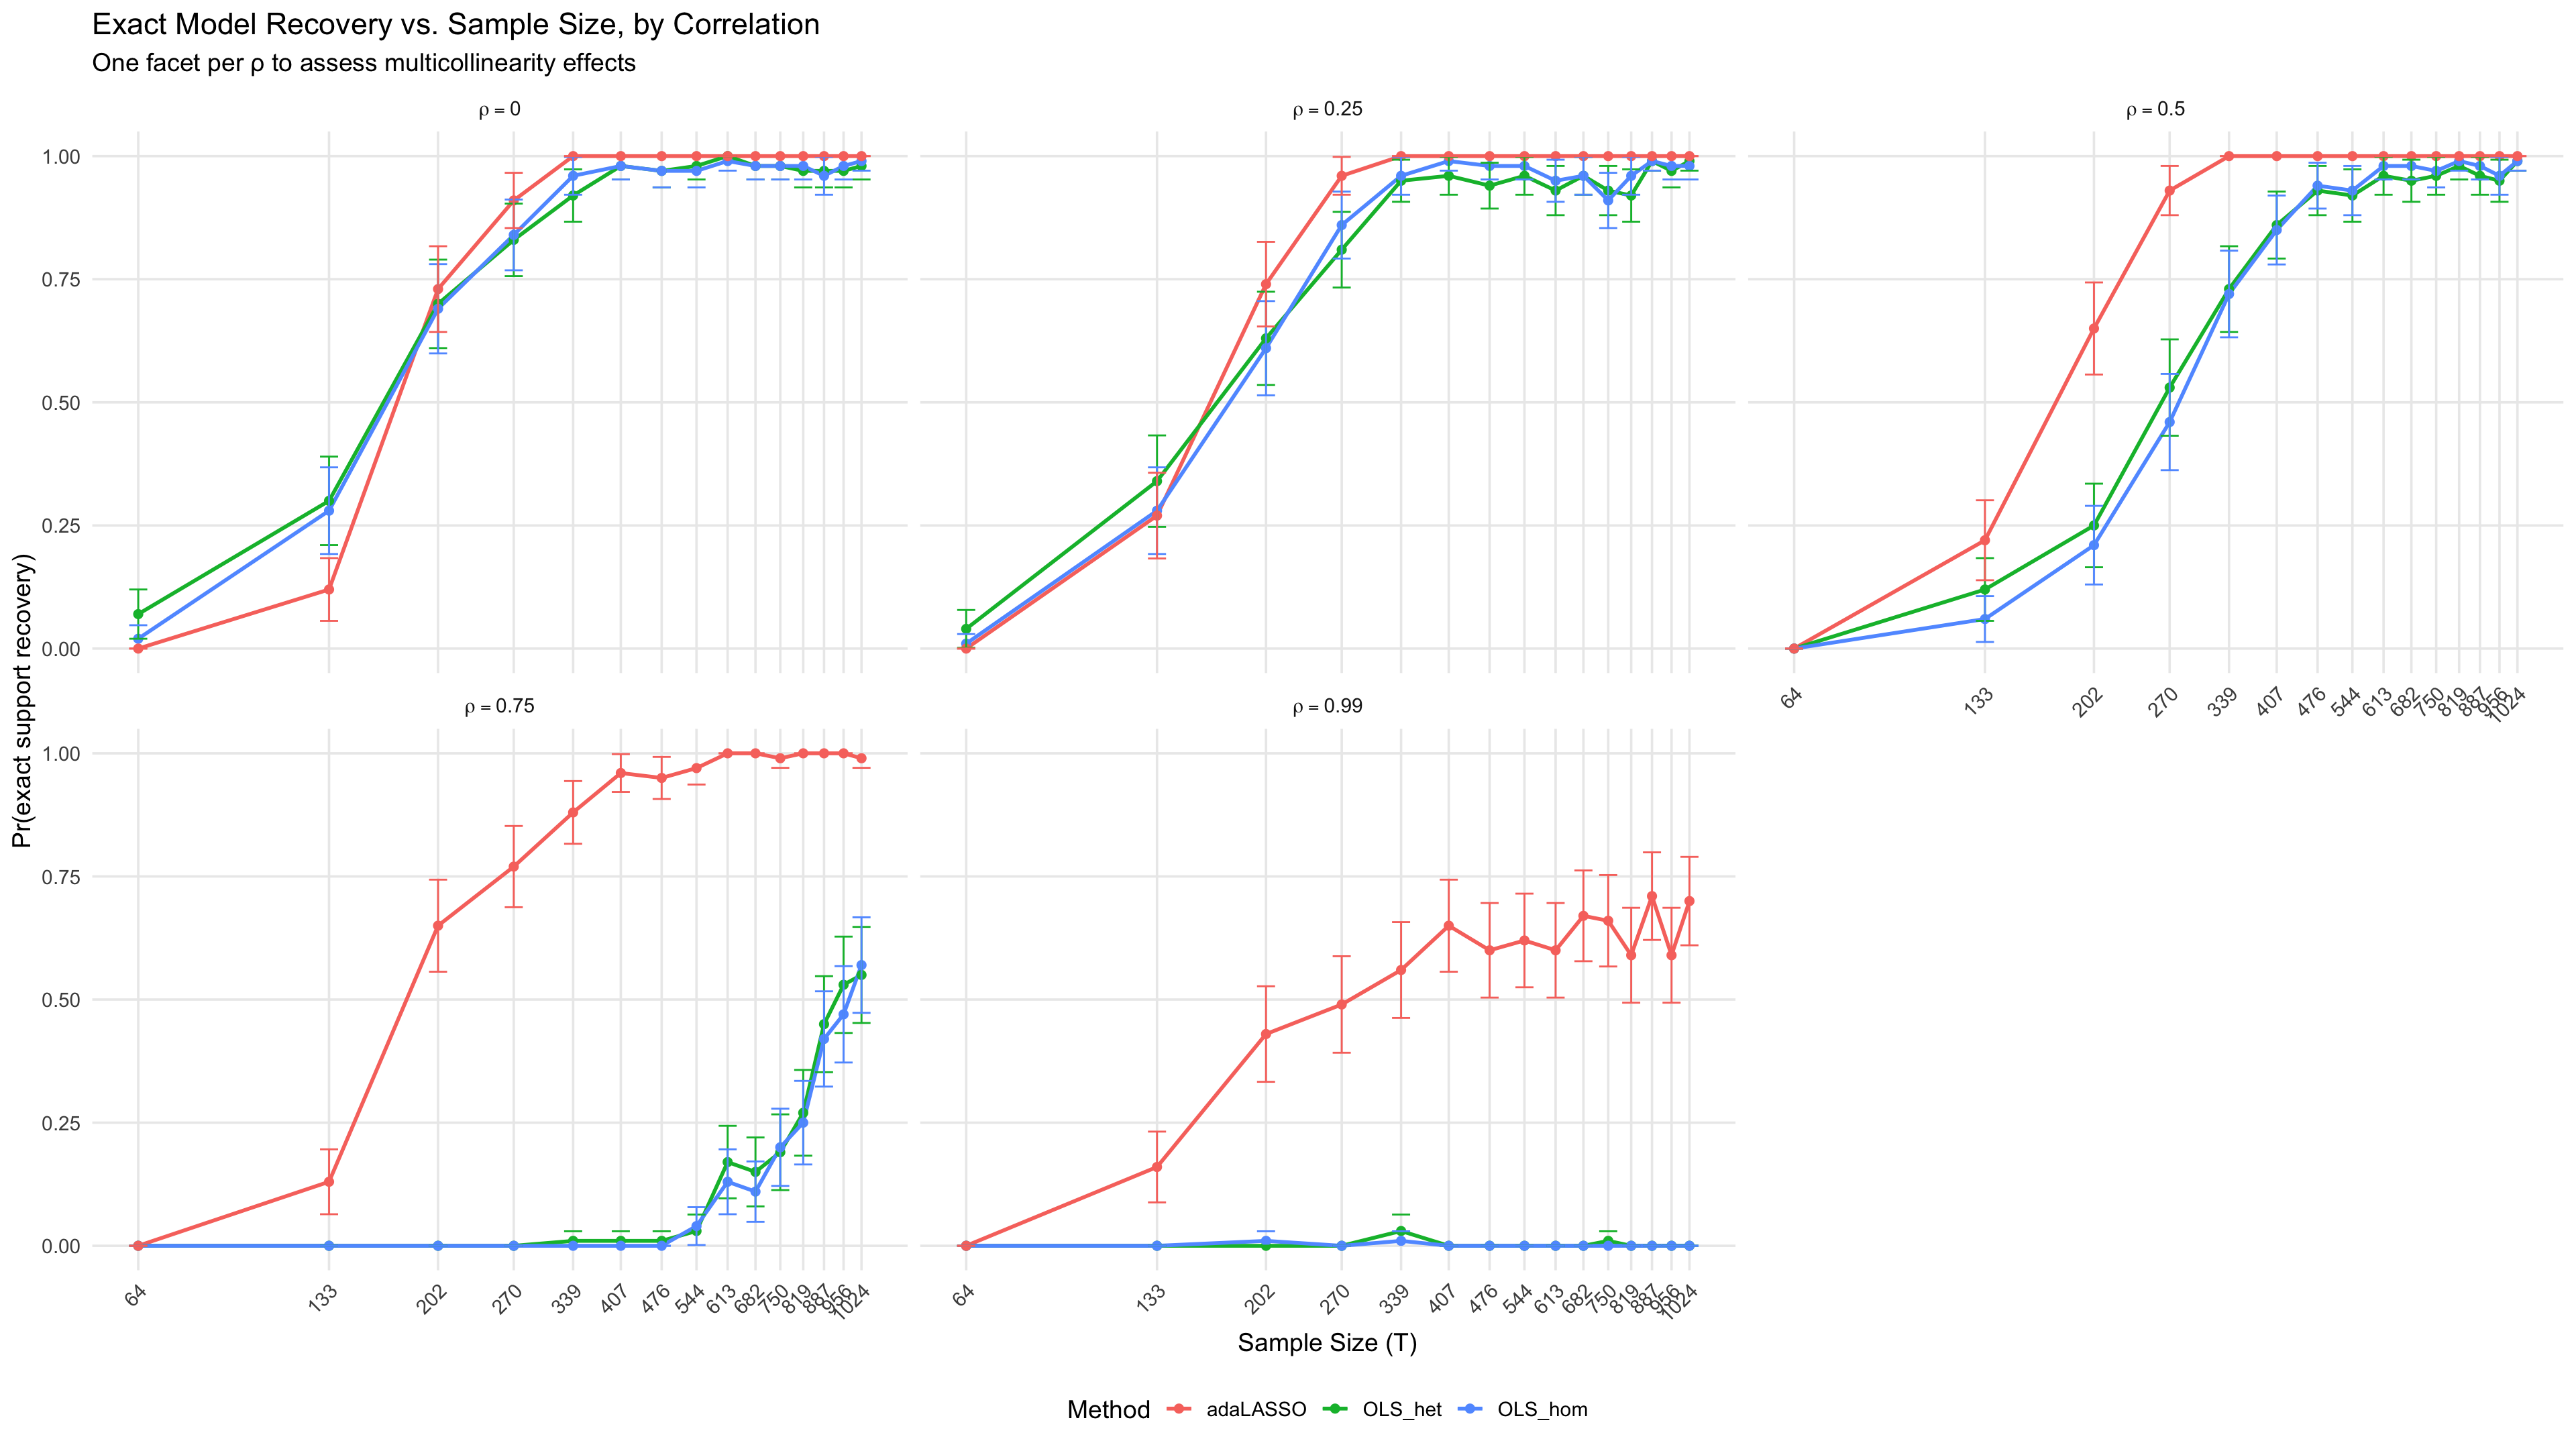
\includegraphics[height=5.5in]{exact_recovery_by_correlation.png}
    \caption{Probability of exact support recovery versus sample size ($T$) for adaptive LASSO (red) and OLS-Bonferroni (blue/green), under varying predictor correlation $\rho$. Each panel corresponds to a different correlation level among predictors (from $\rho=0$ no correlation, up to $\rho=0.99$ extreme collinearity). Error bars (±1.96 SE) are shown for the Monte Carlo estimates.}
    \label{fig:exact_recovery_corr}
\end{sidewaysfigure}

\begin{sidewaysfigure}[h!]
    \centering
    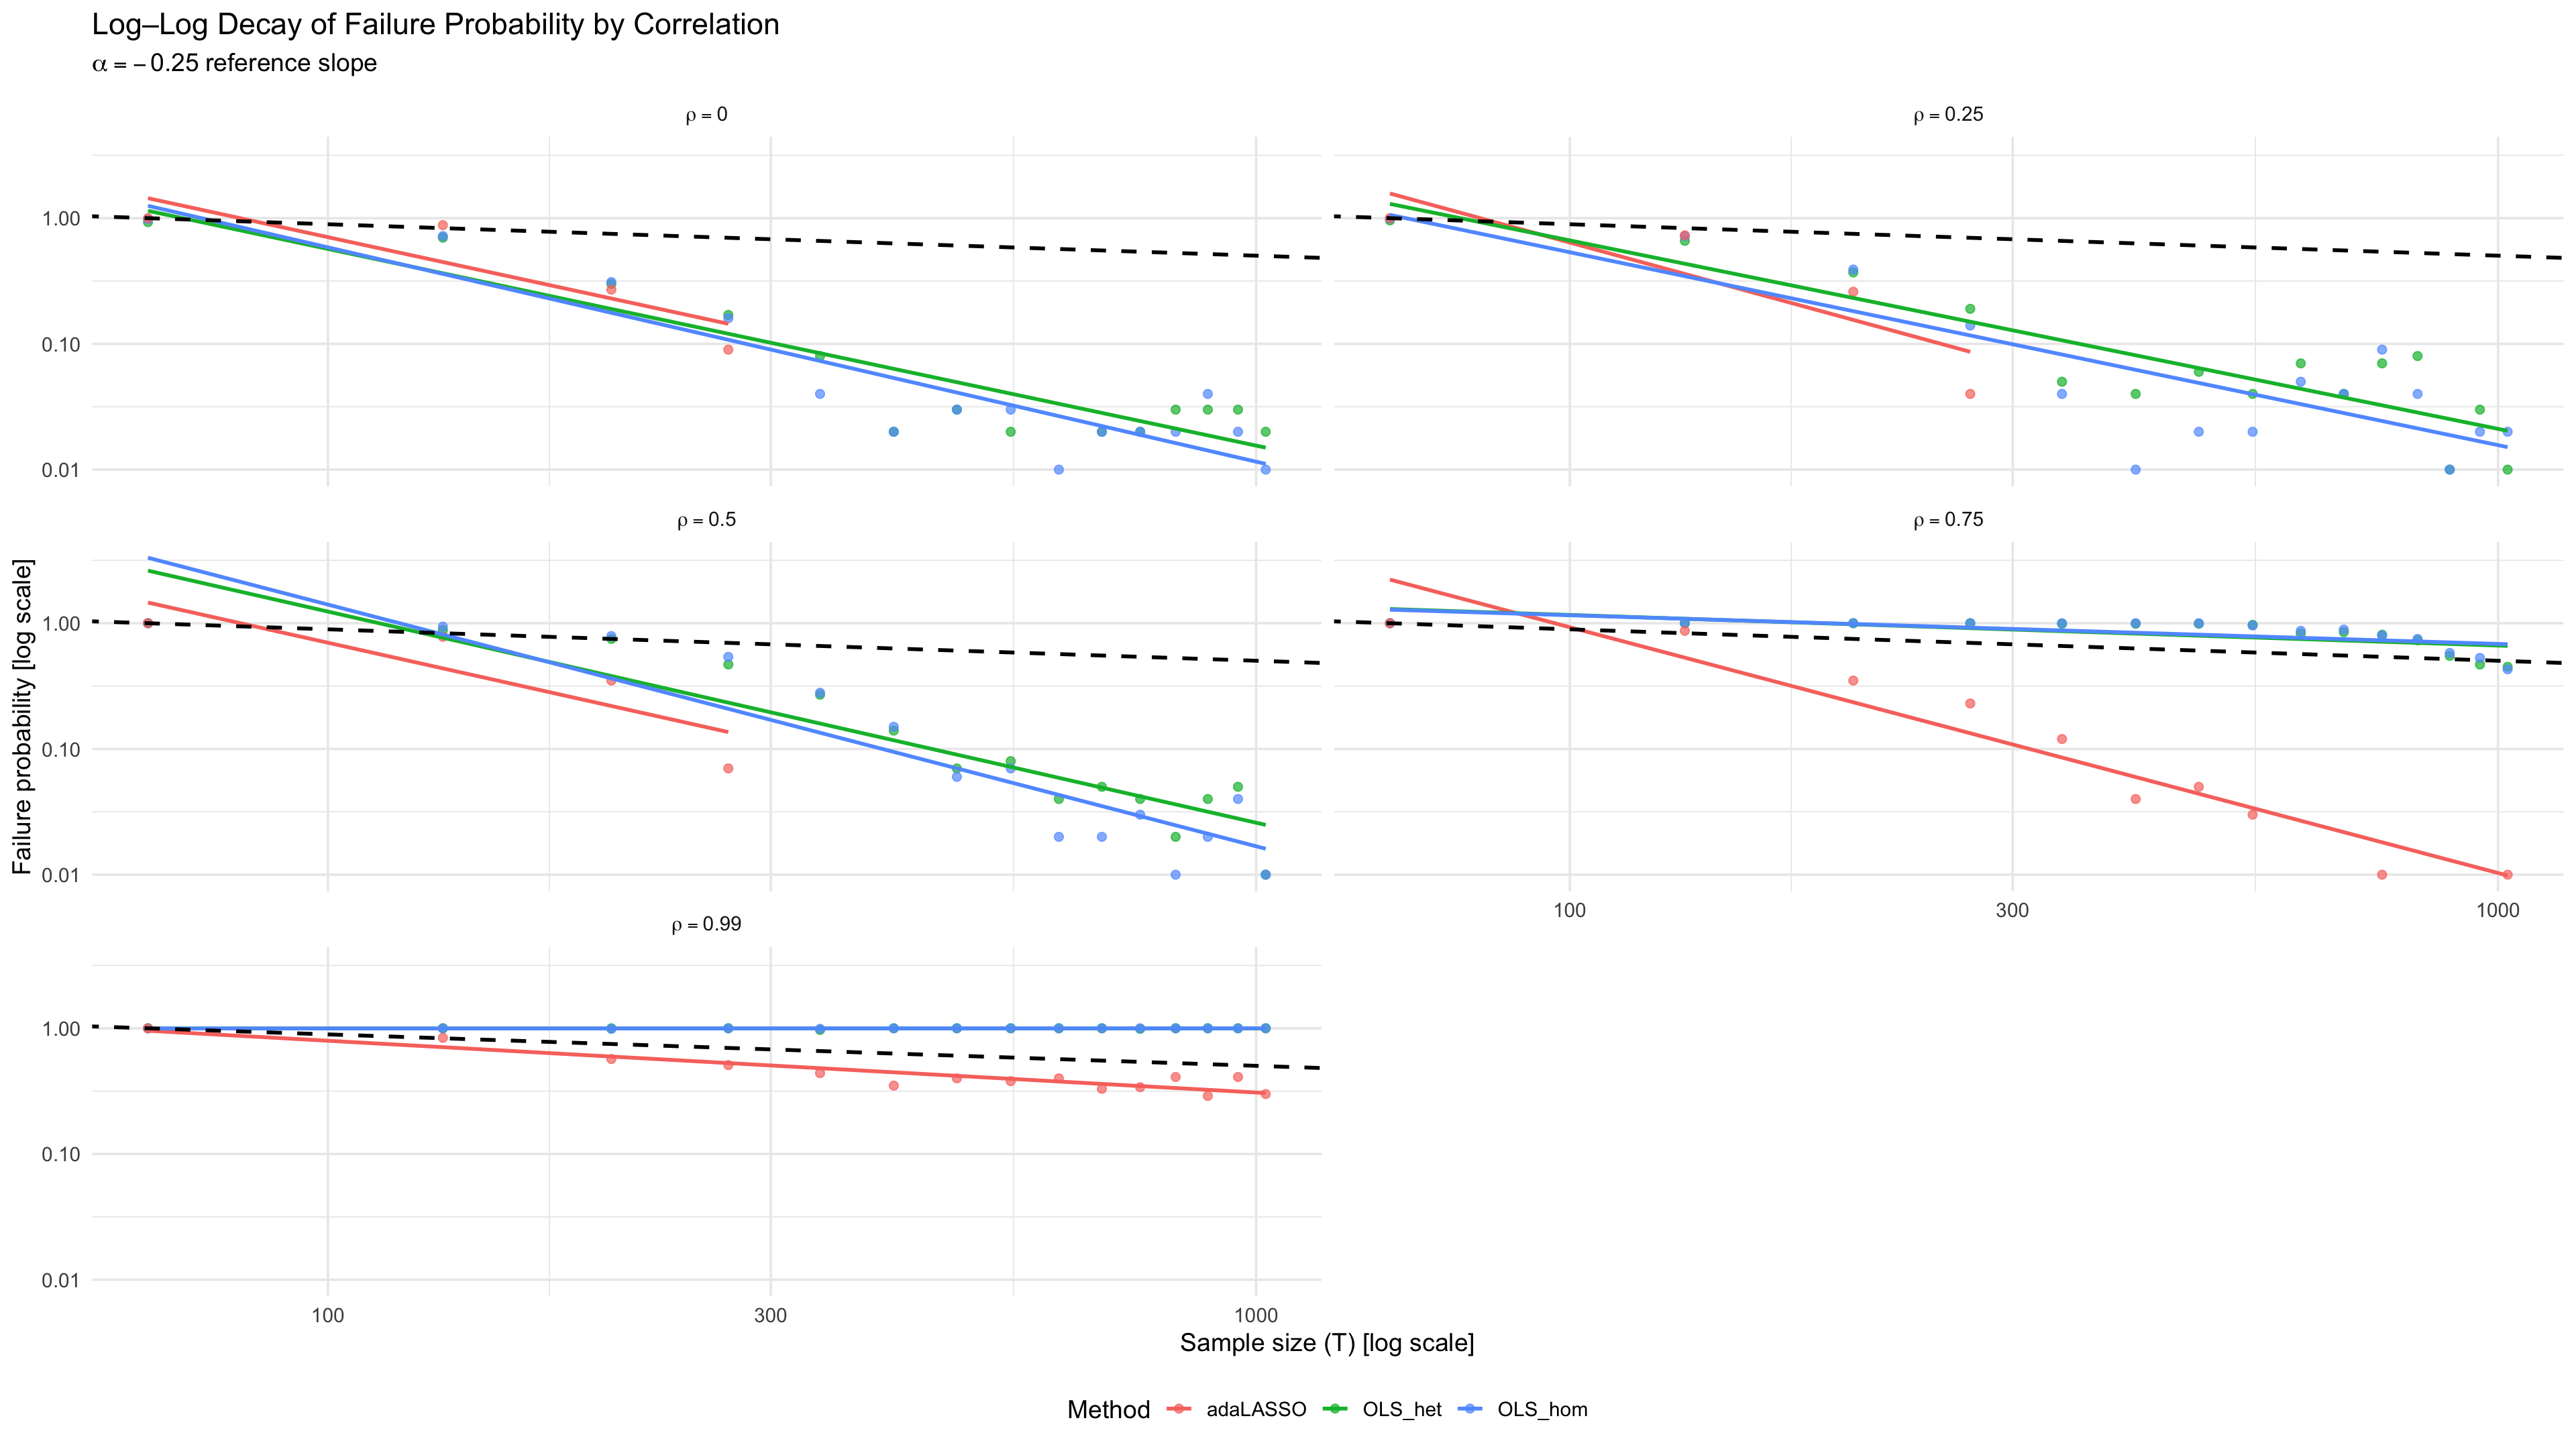
\includegraphics[height=5.5in]{log_log_decay_failure_rate.png}
    \caption{Log–log plot of support recovery failure probability ($\Prob(\mathrm{sign}(\hat{\boldsymbol{\theta}}) \neq \mathrm{sign}(\boldsymbol{\theta}))$) versus sample size $T$, for different correlation levels. Each panel shows the decay of failure probability as $T$ increases on a log–log scale. The red points/line correspond to adaLASSO; blue/green to OLS (homoskedastic or robust OLS, which behave similarly). The black dashed line in each panel indicates a reference slope of $-0.25$ (a power-law $T^{-0.25}$) as a guide.}
    \label{fig:log_log_failure_rate_corr}
\end{sidewaysfigure}

\begin{sidewaysfigure}[h!]
    \centering
    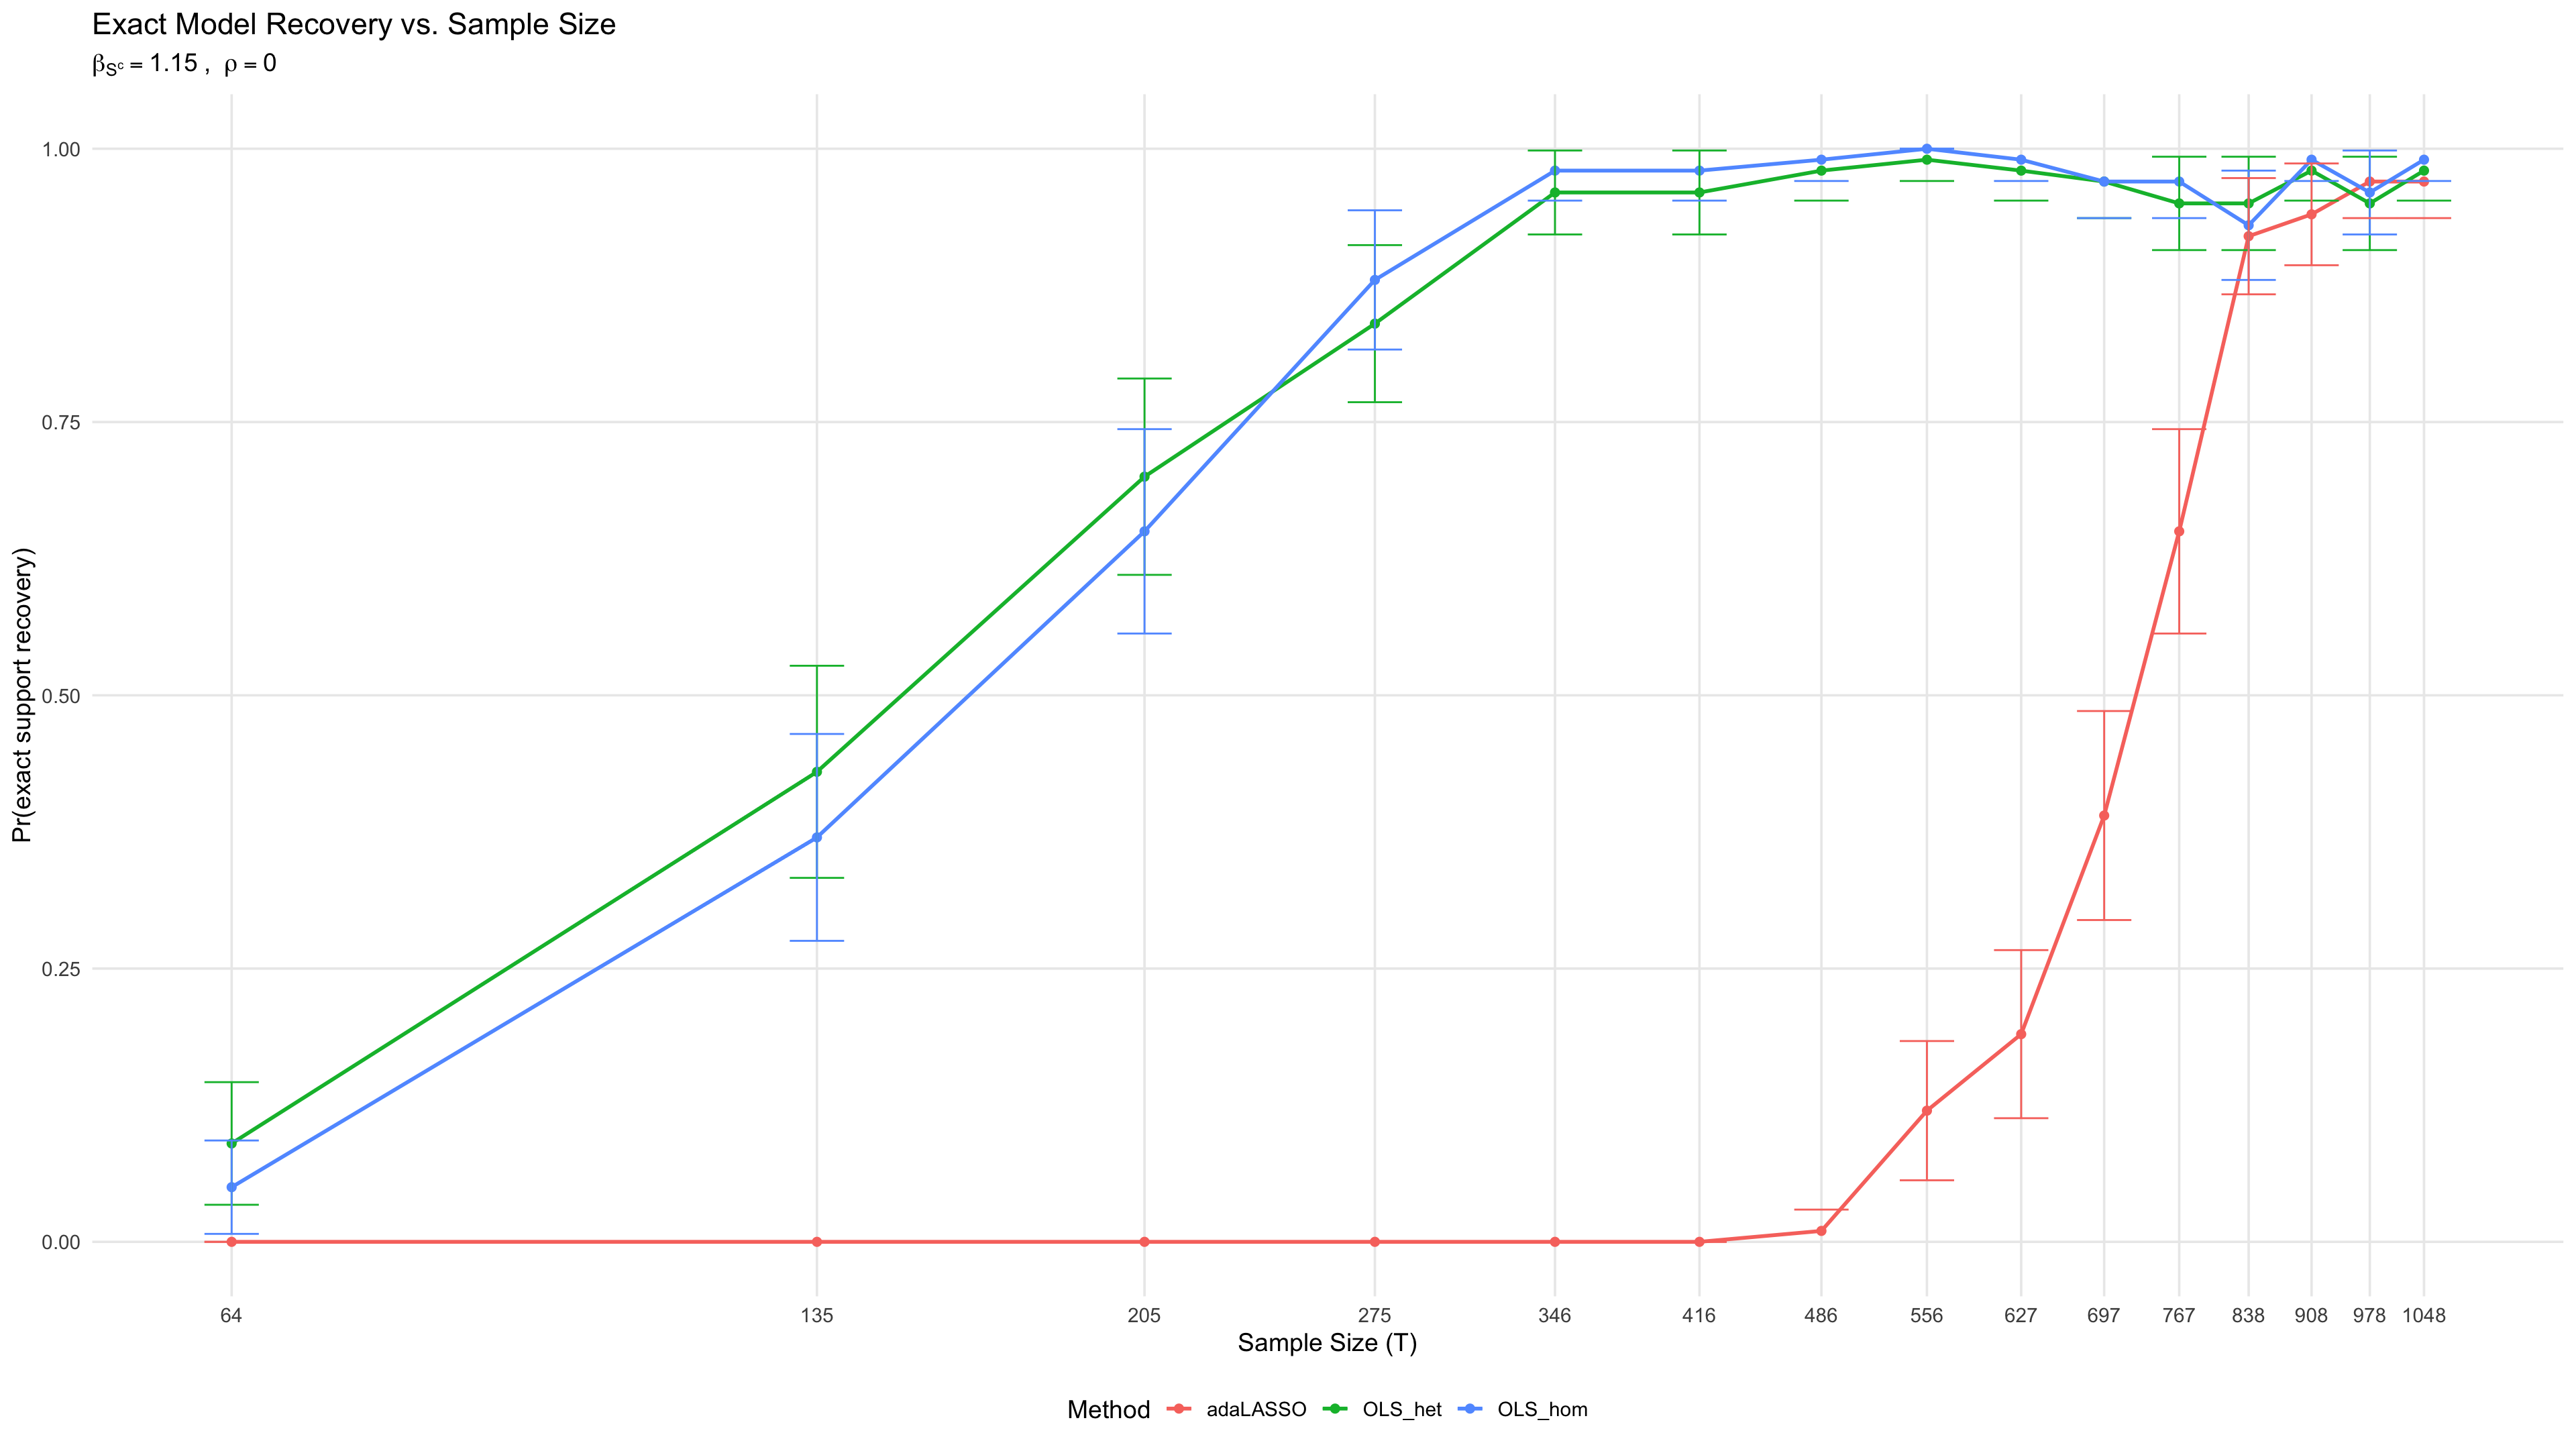
\includegraphics[height=5in]{exact_recovery_low_beta_Sc.png}
    \caption{Probability of exact support recovery versus sample size ($T$) for adaptive LASSO (red) and OLS-Bonferroni (blue/green), under uncorrelated covariates and a comparatively slower discrimination rate $\beta_{S^c} = 1.15$.}
    \label{fig:exact_recovery_beta}
\end{sidewaysfigure}

\begin{sidewaysfigure}[h!]
    \centering
    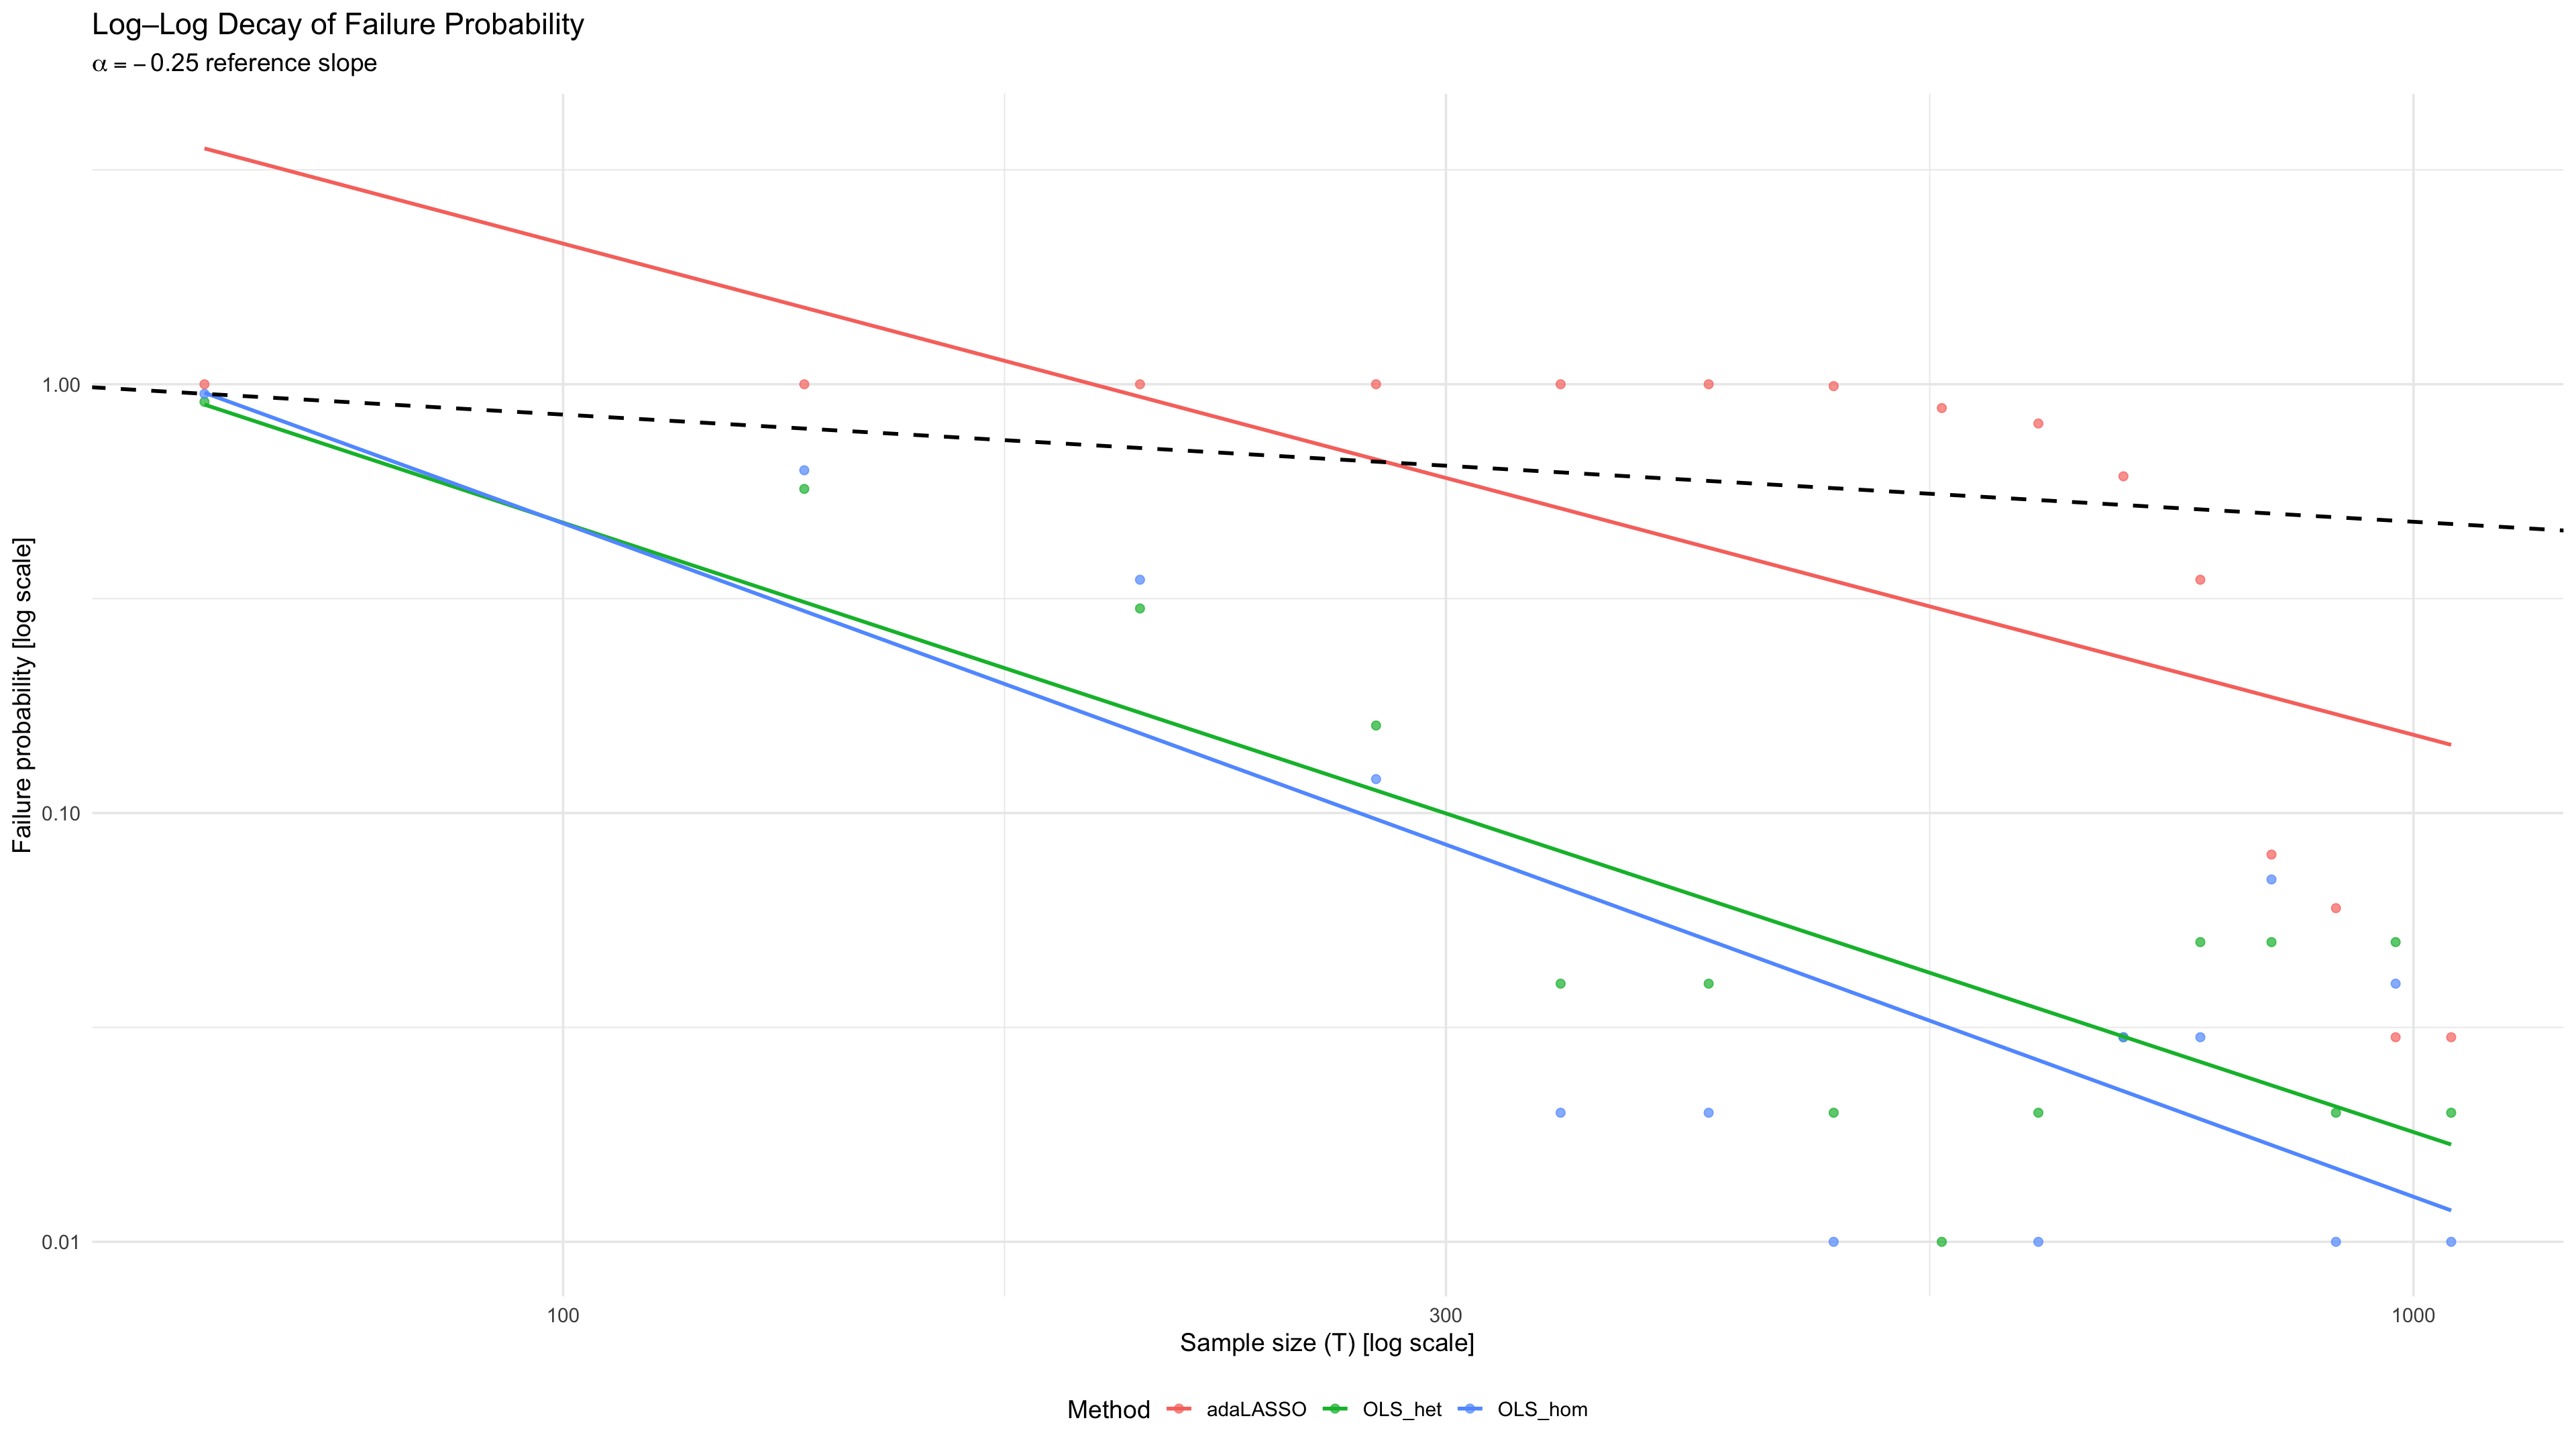
\includegraphics[height=5in]{log_log_decay_low_beta_sc.png}
    \caption{Log–log plot of support recovery failure probability ($\Prob(\mathrm{sign}(\hat{\boldsymbol{\theta}}) \neq \mathrm{sign}(\boldsymbol{\theta}))$) versus sample size $T$, assuming uncorrelated variables and a comparatively slower discrimination rate $\beta_{S^c} = 1.15$.}
    \label{fig:log_log_failure_rate_beta}
\end{sidewaysfigure}

% Please add the following packages to your preamble:
% \usepackage{booktabs}
% \usepackage{multirow}
% \usepackage{longtable}

\begin{longtable}{@{}lll@{}}
\caption{Base configuration used in synthetic data experiments.} 
\label{tab:base_config} \\
\toprule
\textbf{Category} & \textbf{Parameter} & \textbf{Value} \\ \midrule
\endfirsthead

\multicolumn{3}{c}%
{{\bfseries Table \thetable\ (continued)}} \\
\toprule
\textbf{Category} & \textbf{Parameter} & \textbf{Value} \\ \midrule
\endhead

\bottomrule
\endfoot

\multirow{8}{*}{General} 
 & Ticker & SIM (Simulated LOB) \\
 & $\Delta^B$ & $5{'}000{,}000.0$ uot \\
 & $\Delta^A$ & $100{,}000.0$ uot \\
 & $\delta$ & $100.0$ uot \\
 & Seed & 19991810 \\
 & Session start & 0.0 uot \\
 & Session finish & $10{'}000{,}000.0$ uot \\
 & Target Variable & $r^w$ \\ \midrule

\multirow{10}{*}{Backbone} 
 & Training Epochs & 10 \\
 & Batch size & 32 \\
 & Validation proportion & 0.1 \\
 & Buffer proportion & 0.05 \\
 & Windsorization quantile & 0.005 \\
 & ADF rejection threshold & 0.8 \\
 & KPSS verification threshold & 0.2 \\
 & NA threshold & 0.1 \\
 & Learning rate & 0.0001 \\
 & Correlation threshold & 0.95 \\ \midrule

\multirow{9}{*}{Interface} 
 & $\alpha$  & \{0.0, 0.1, 0.25, 0.5, 0.75, 0.9, 1.0\} \\
 & $\lambda_1$ & $\mathrm{logspace}(-4,1,25)$ \\
 & $\tau$   & \{0.25, 0.5, 1.0, 1.5, 2.0\} \\
 & $\lambda_2$ & $\mathrm{logspace}(0,1,25)$ \\
 & Validation proportion & 0.2 \\
 & Selection threshold & 0.17 ($L = 50$, $\alpha = 0.00005$) \\
 & Tolerance threshold & $10^{-6}$ \\
 & OLS significance level & 0.05 \\
 & Surrogate model lags & 5 \\ \midrule

\multirow{3}{*}{Adapter} 
 & ARMA order & (1,1) \\
 & GARCH order & (1,1) \\
 & Error distribution & Skewed t \\
\end{longtable} 

\begin{figure}[ht!]
\centering

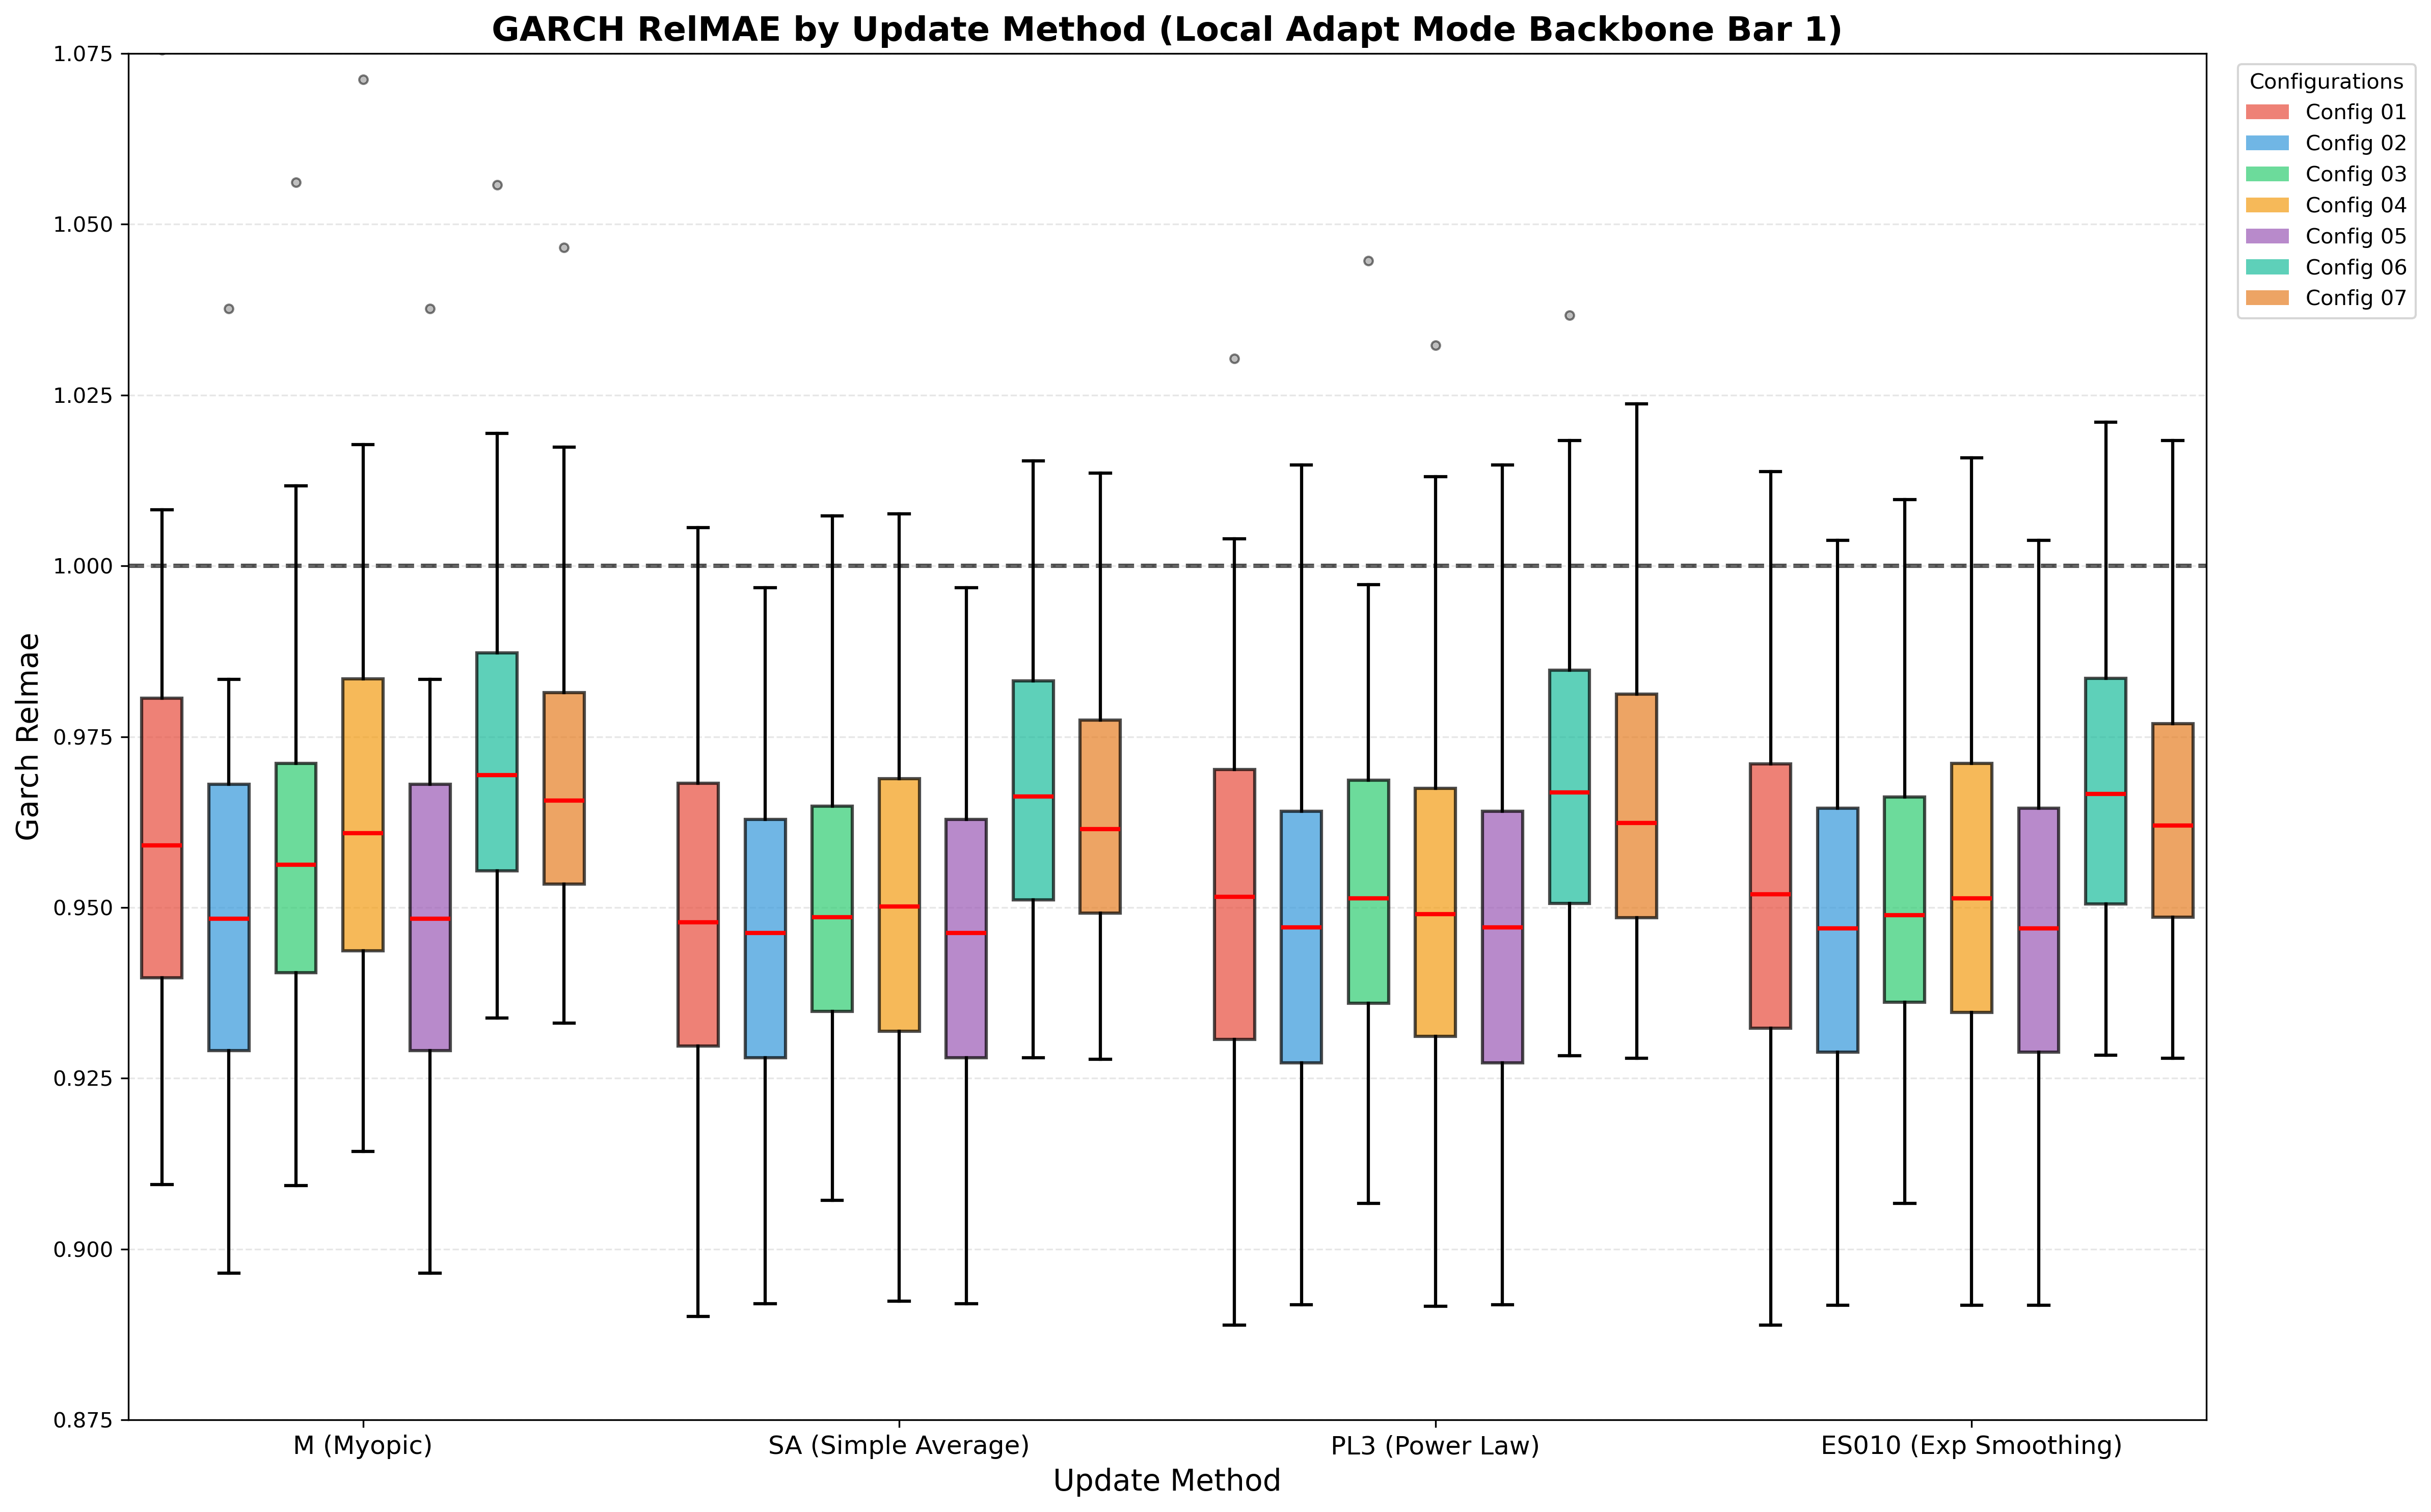
\includegraphics[width=0.85\linewidth]{performance_boxplot_bb000.png}
\vspace{0.5em}
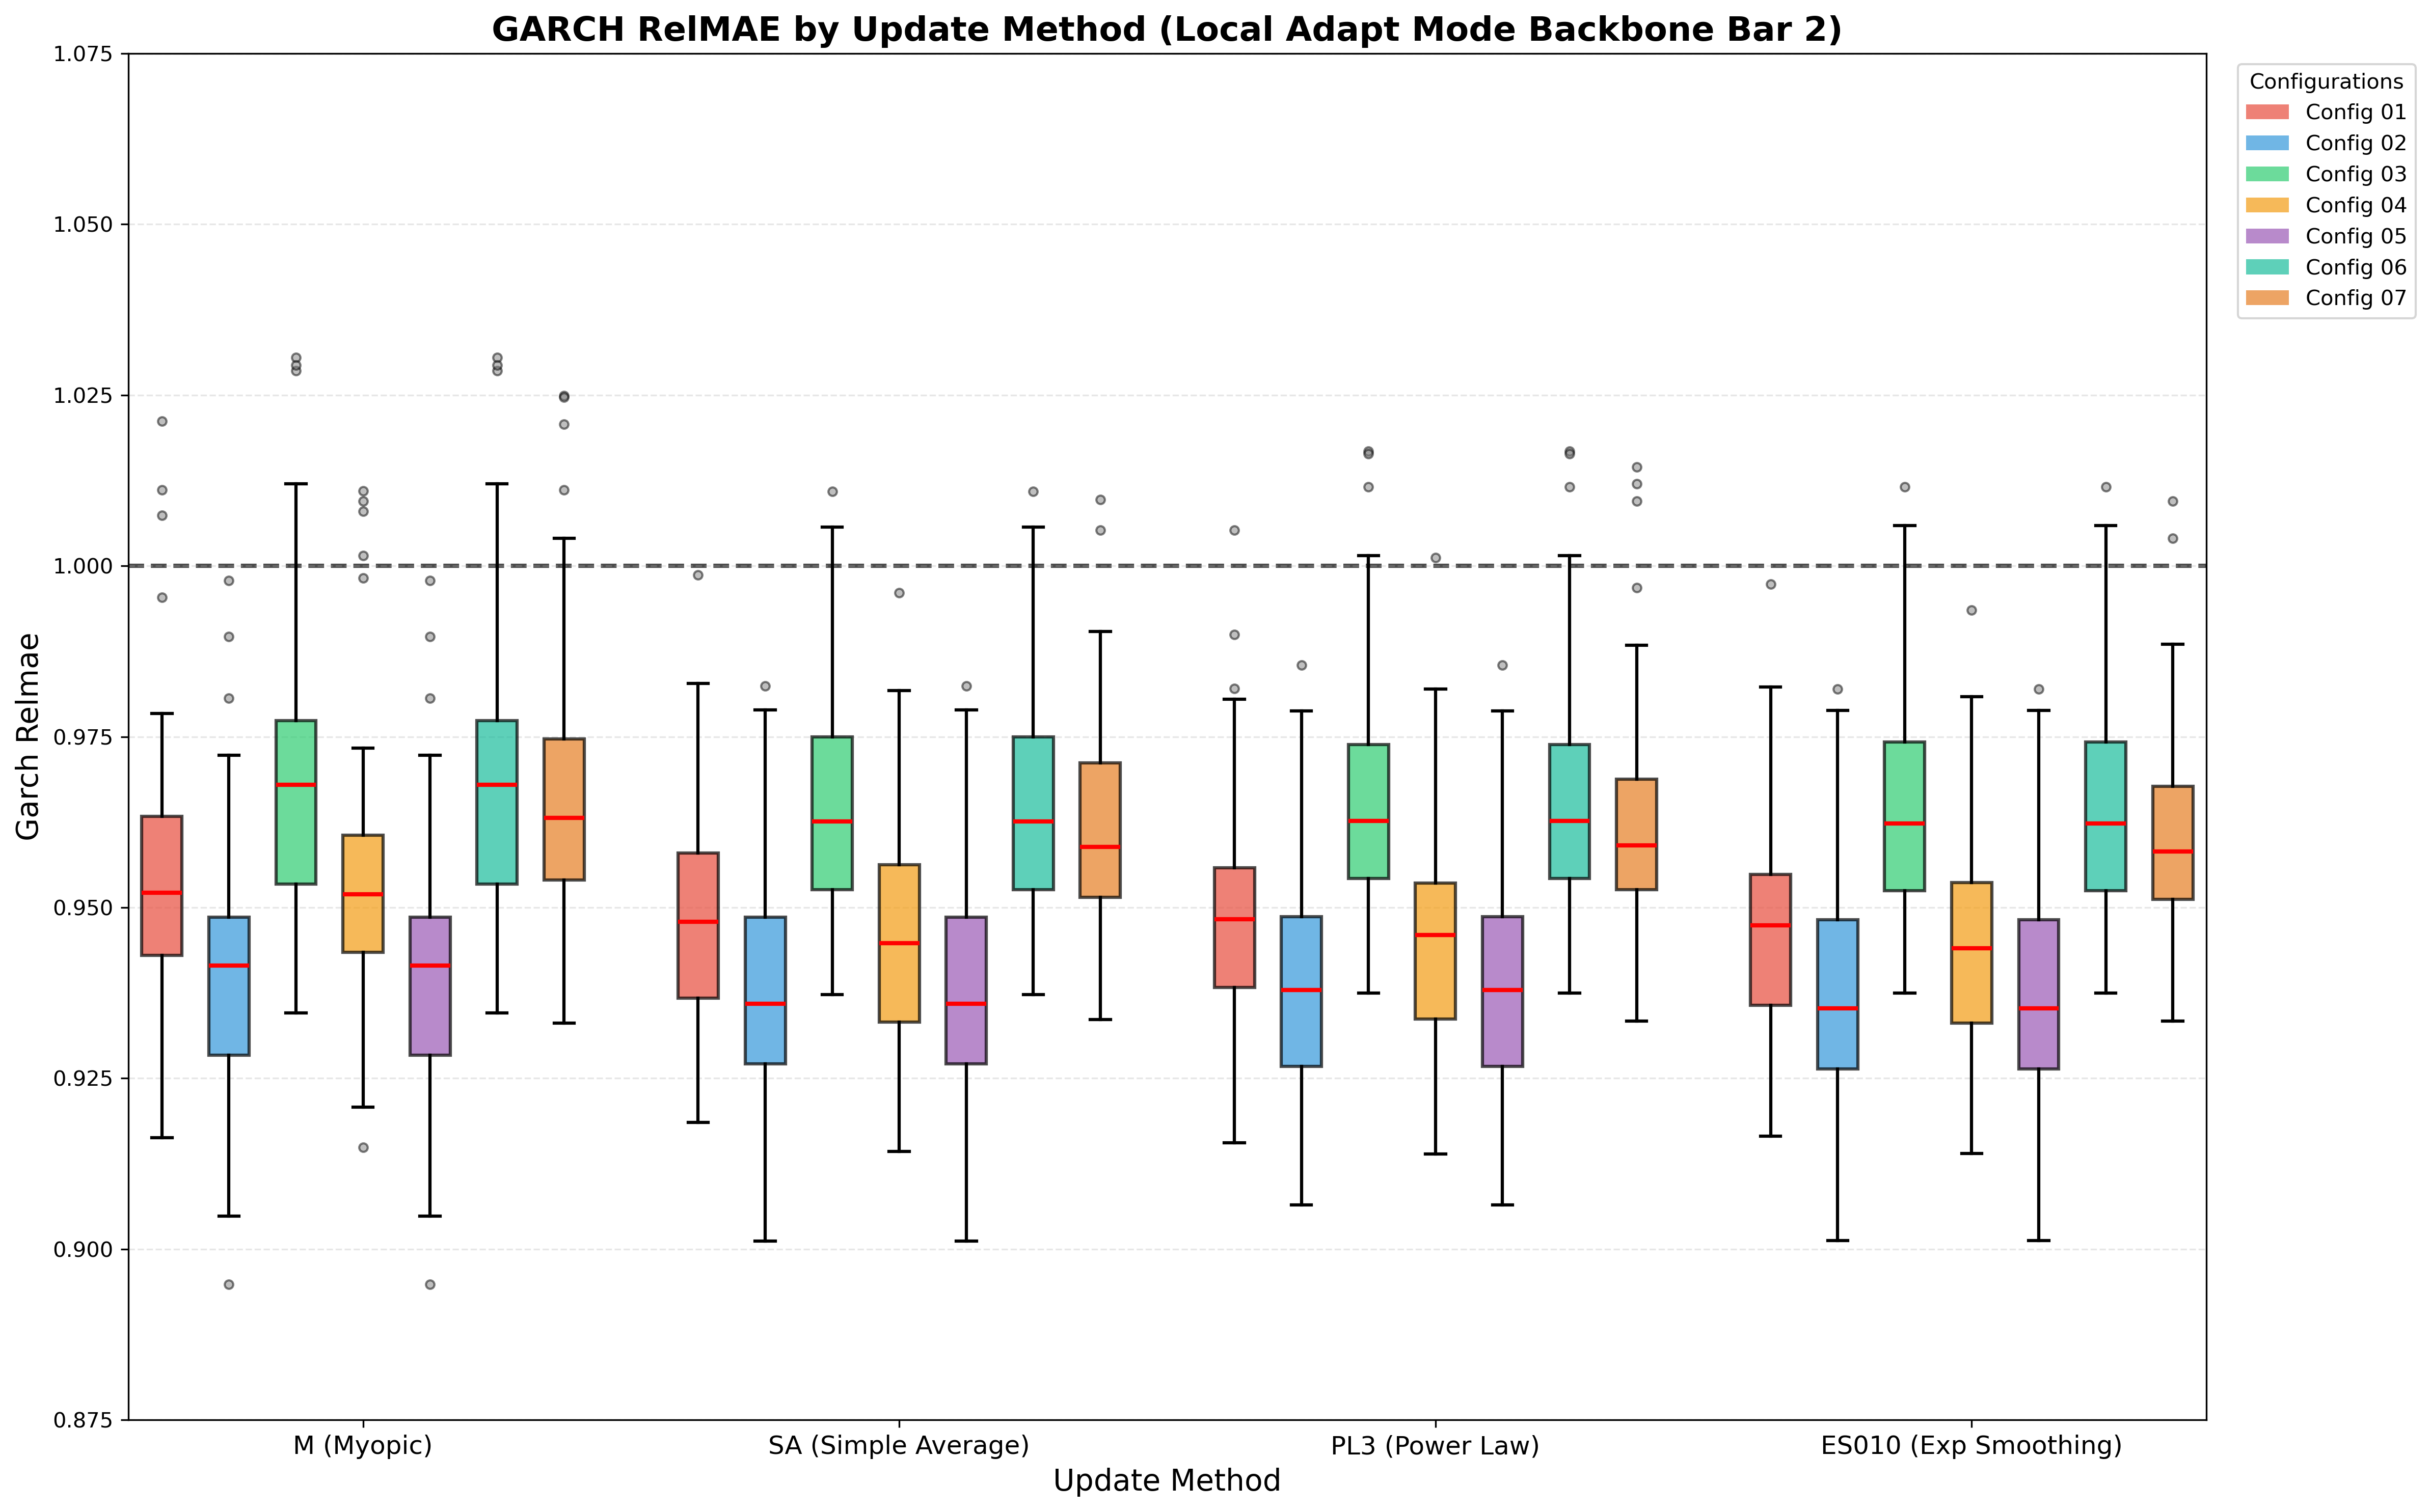
\includegraphics[width=0.85\linewidth]{performance_boxplot_bb001.png}

\caption{GARCH RelMAE comparison across update methods and configurations.}
\label{fig:garch_relmae_vertical}
\end{figure}

\begin{figure}[ht!]
\centering

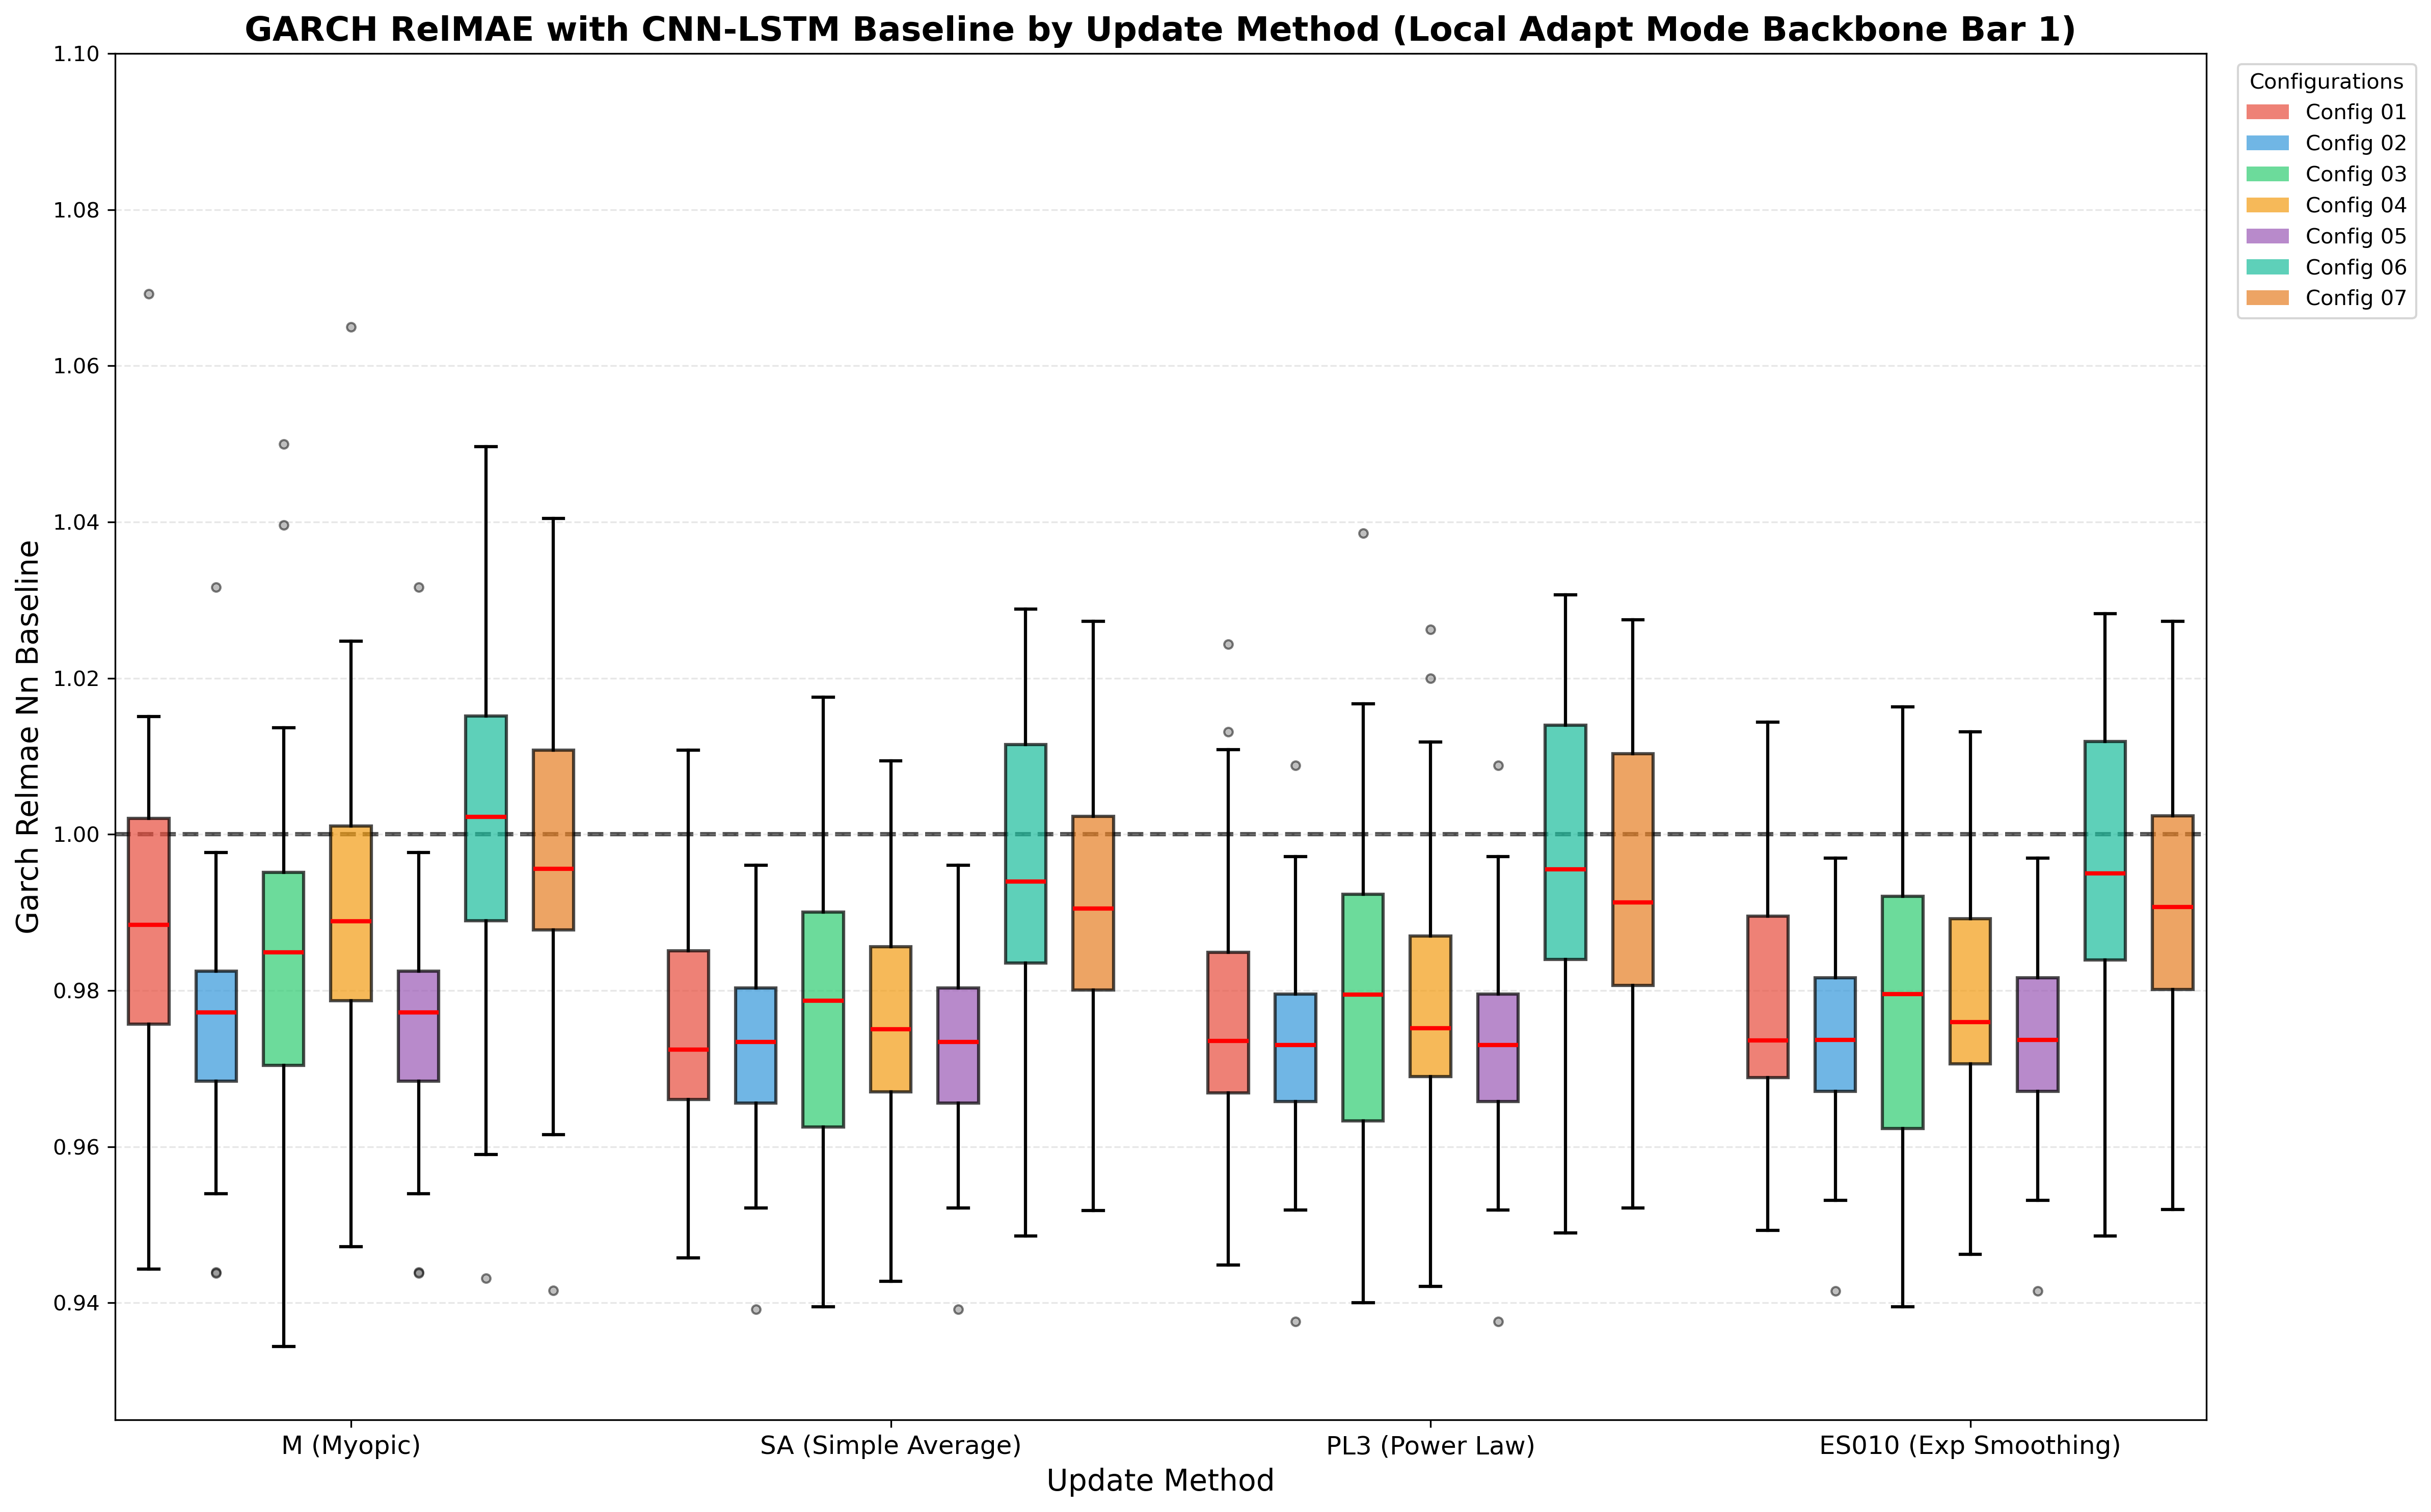
\includegraphics[width=0.85\linewidth]{performance_boxplot_bb000_nn_baseline.png}
\vspace{0.5em}
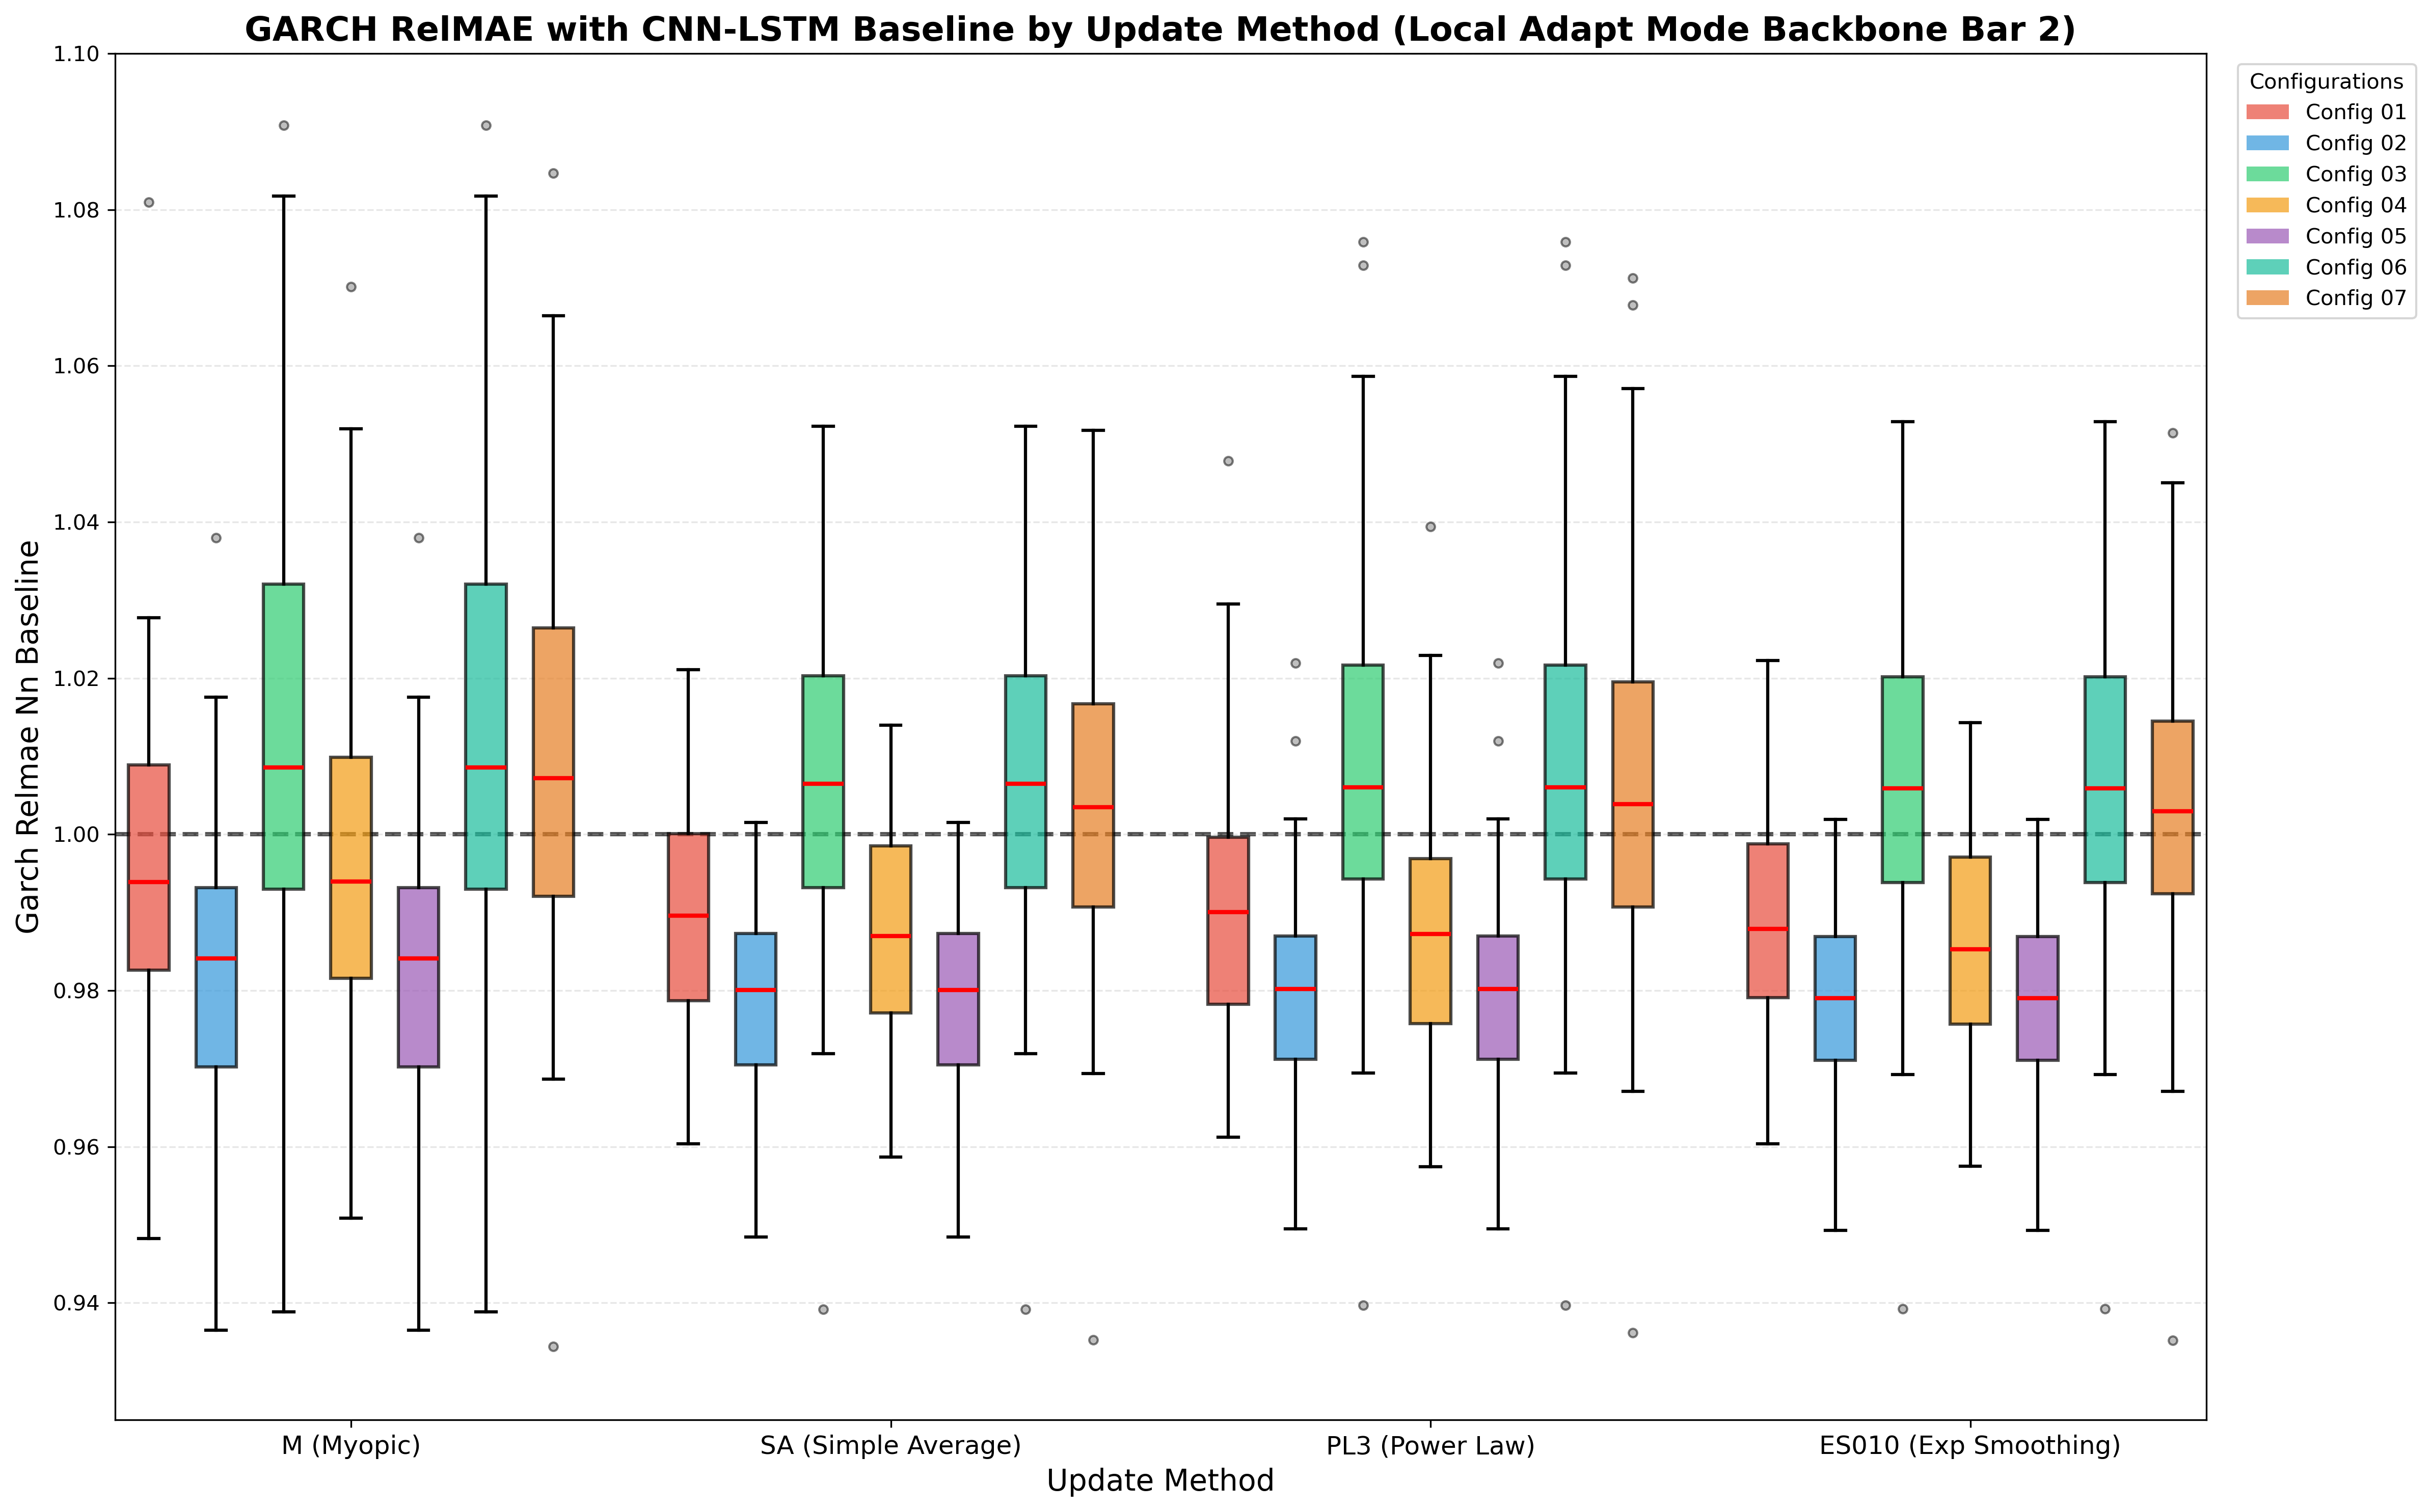
\includegraphics[width=0.85\linewidth]{performance_boxplot_bb001_nn_baseline.png}

\caption{GARCH RelMAE comparison across update methods and configurations with CNN-LSTM baseline.}
\label{fig:garch_relmae_cnn_lstm_baseline_vertical}
\end{figure}


\begin{figure}[htb]
  \centering
  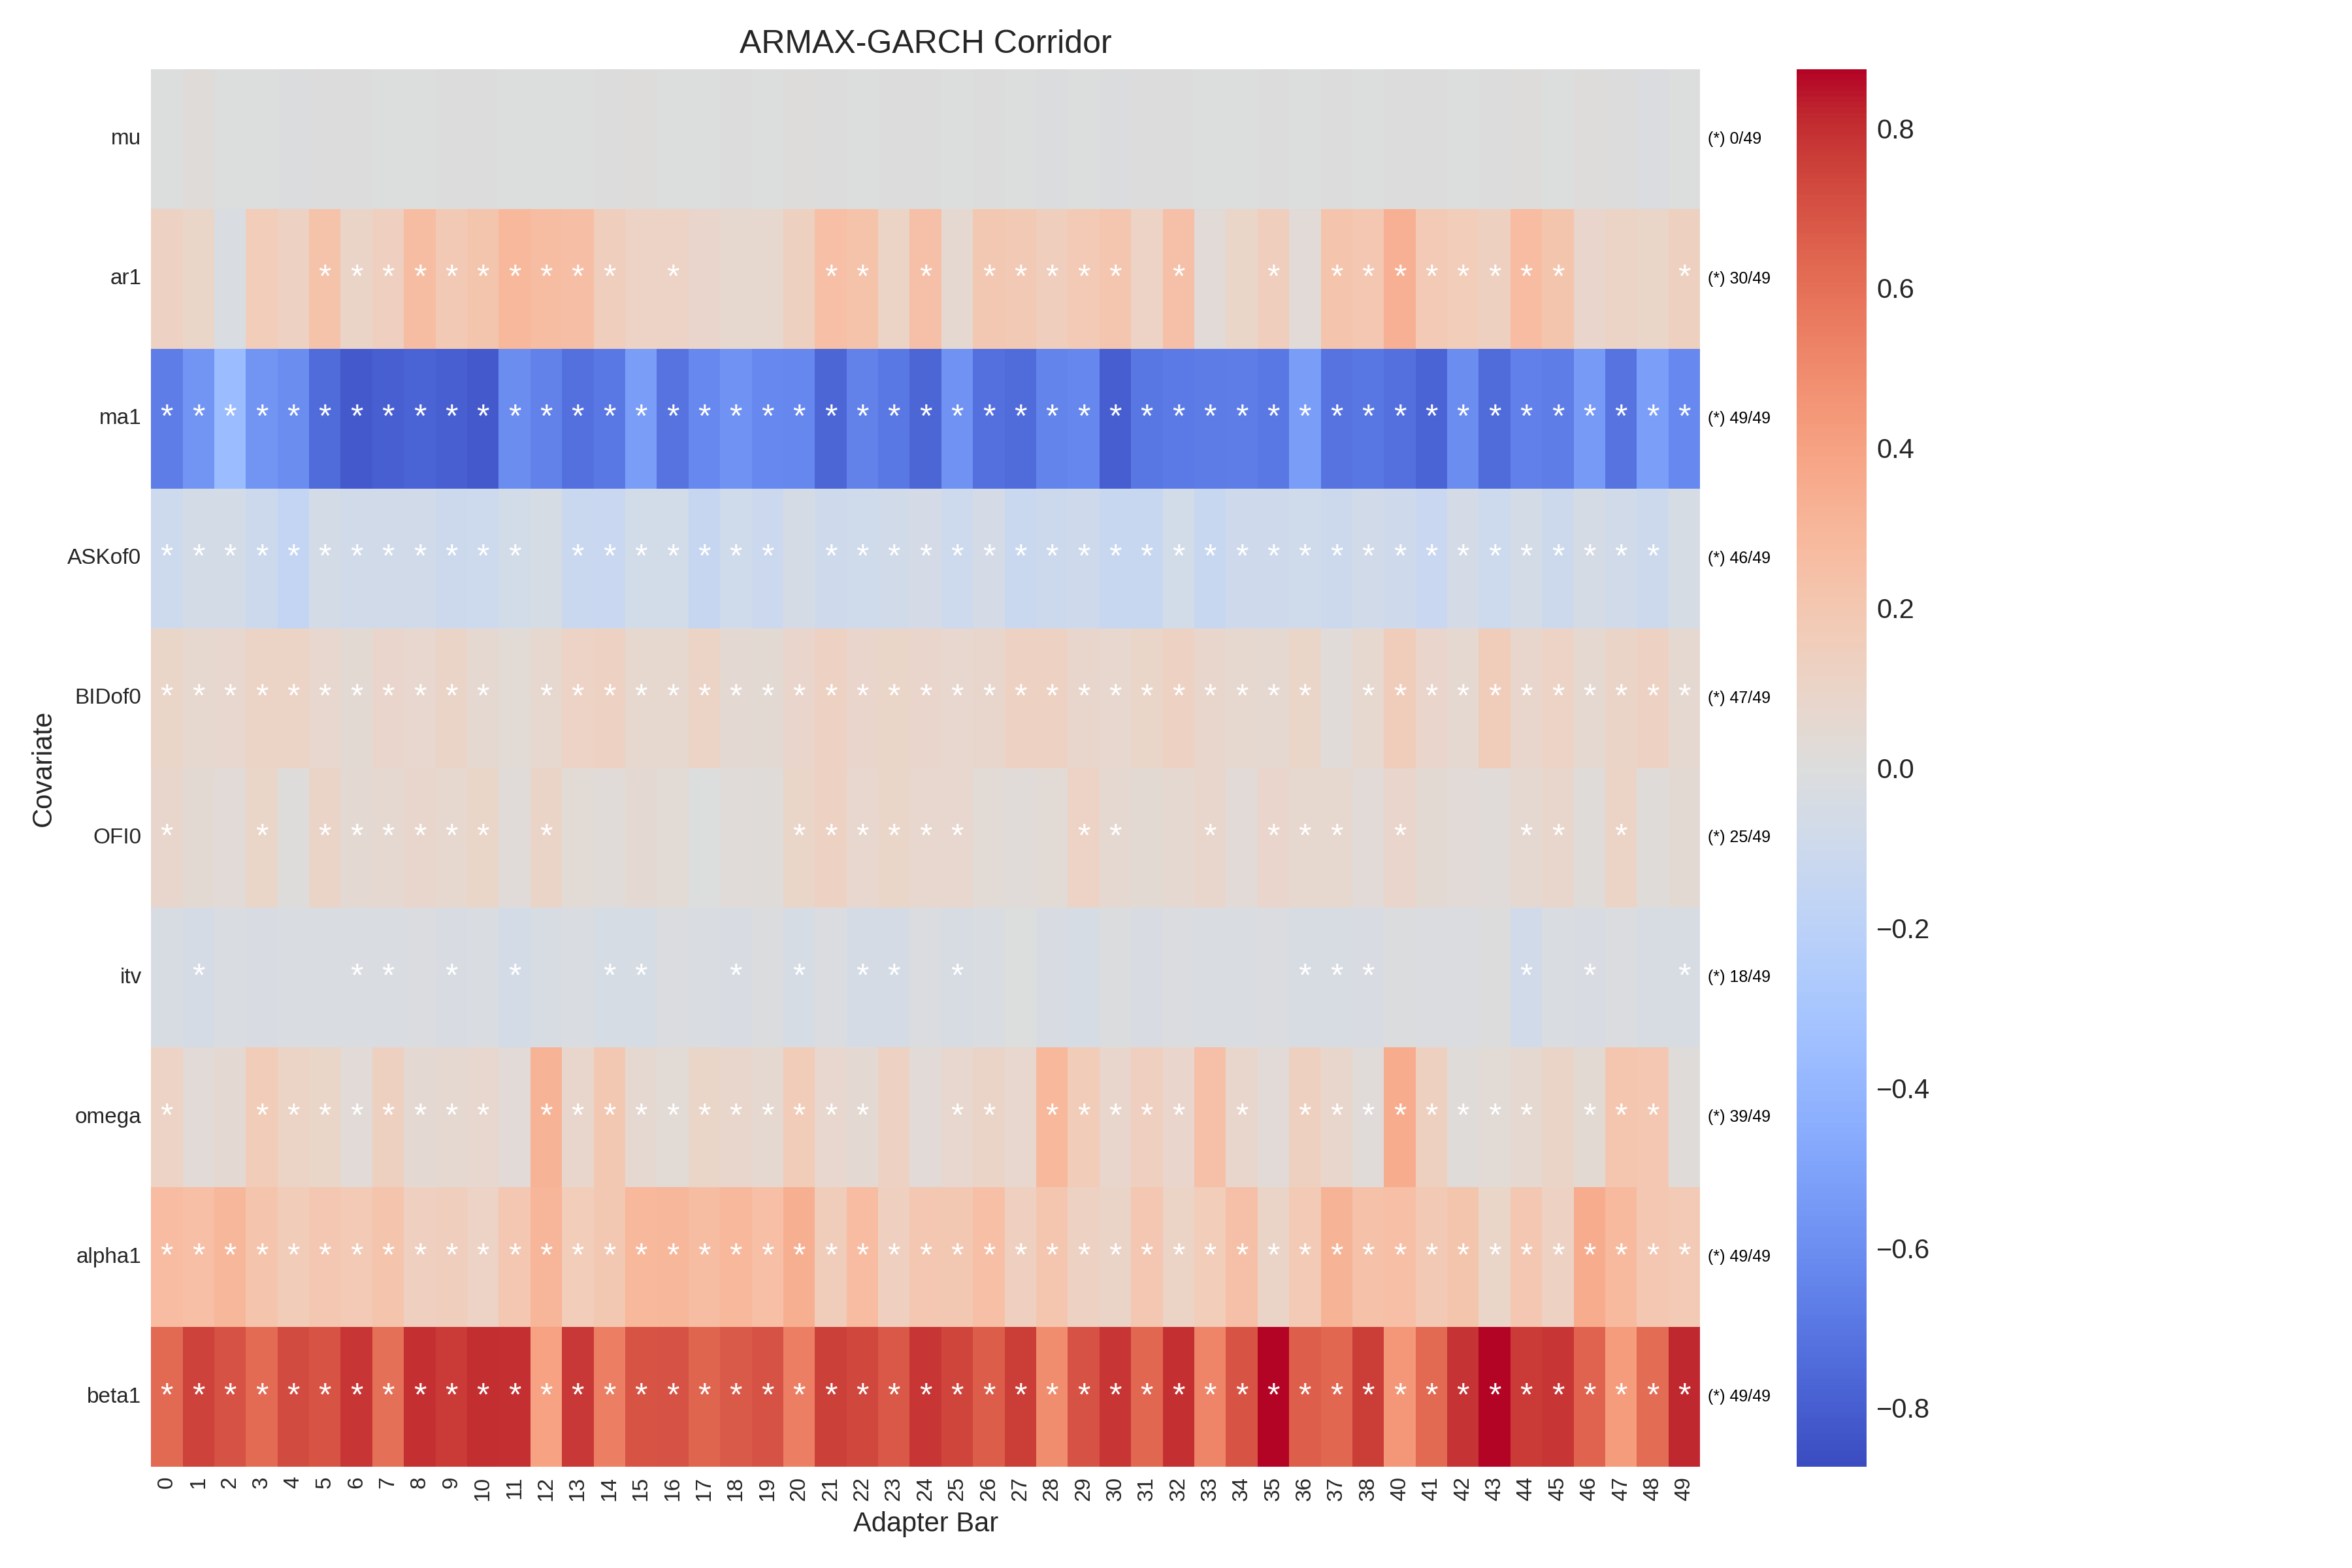
\includegraphics[width=\linewidth]{armax_garch_corridor_SA_03_synthetic_data.png}
  \caption{ARMAX–GARCH-DeepLOB corridor for configuration \texttt{SA\_03}. Cells show bar-specific coefficient magnitudes by adapter bar; asterisks mark statistical significance.}
  \label{fig:armax_garch_corridor_sa_03}
\end{figure}

\begin{figure}[htb]
  \centering
  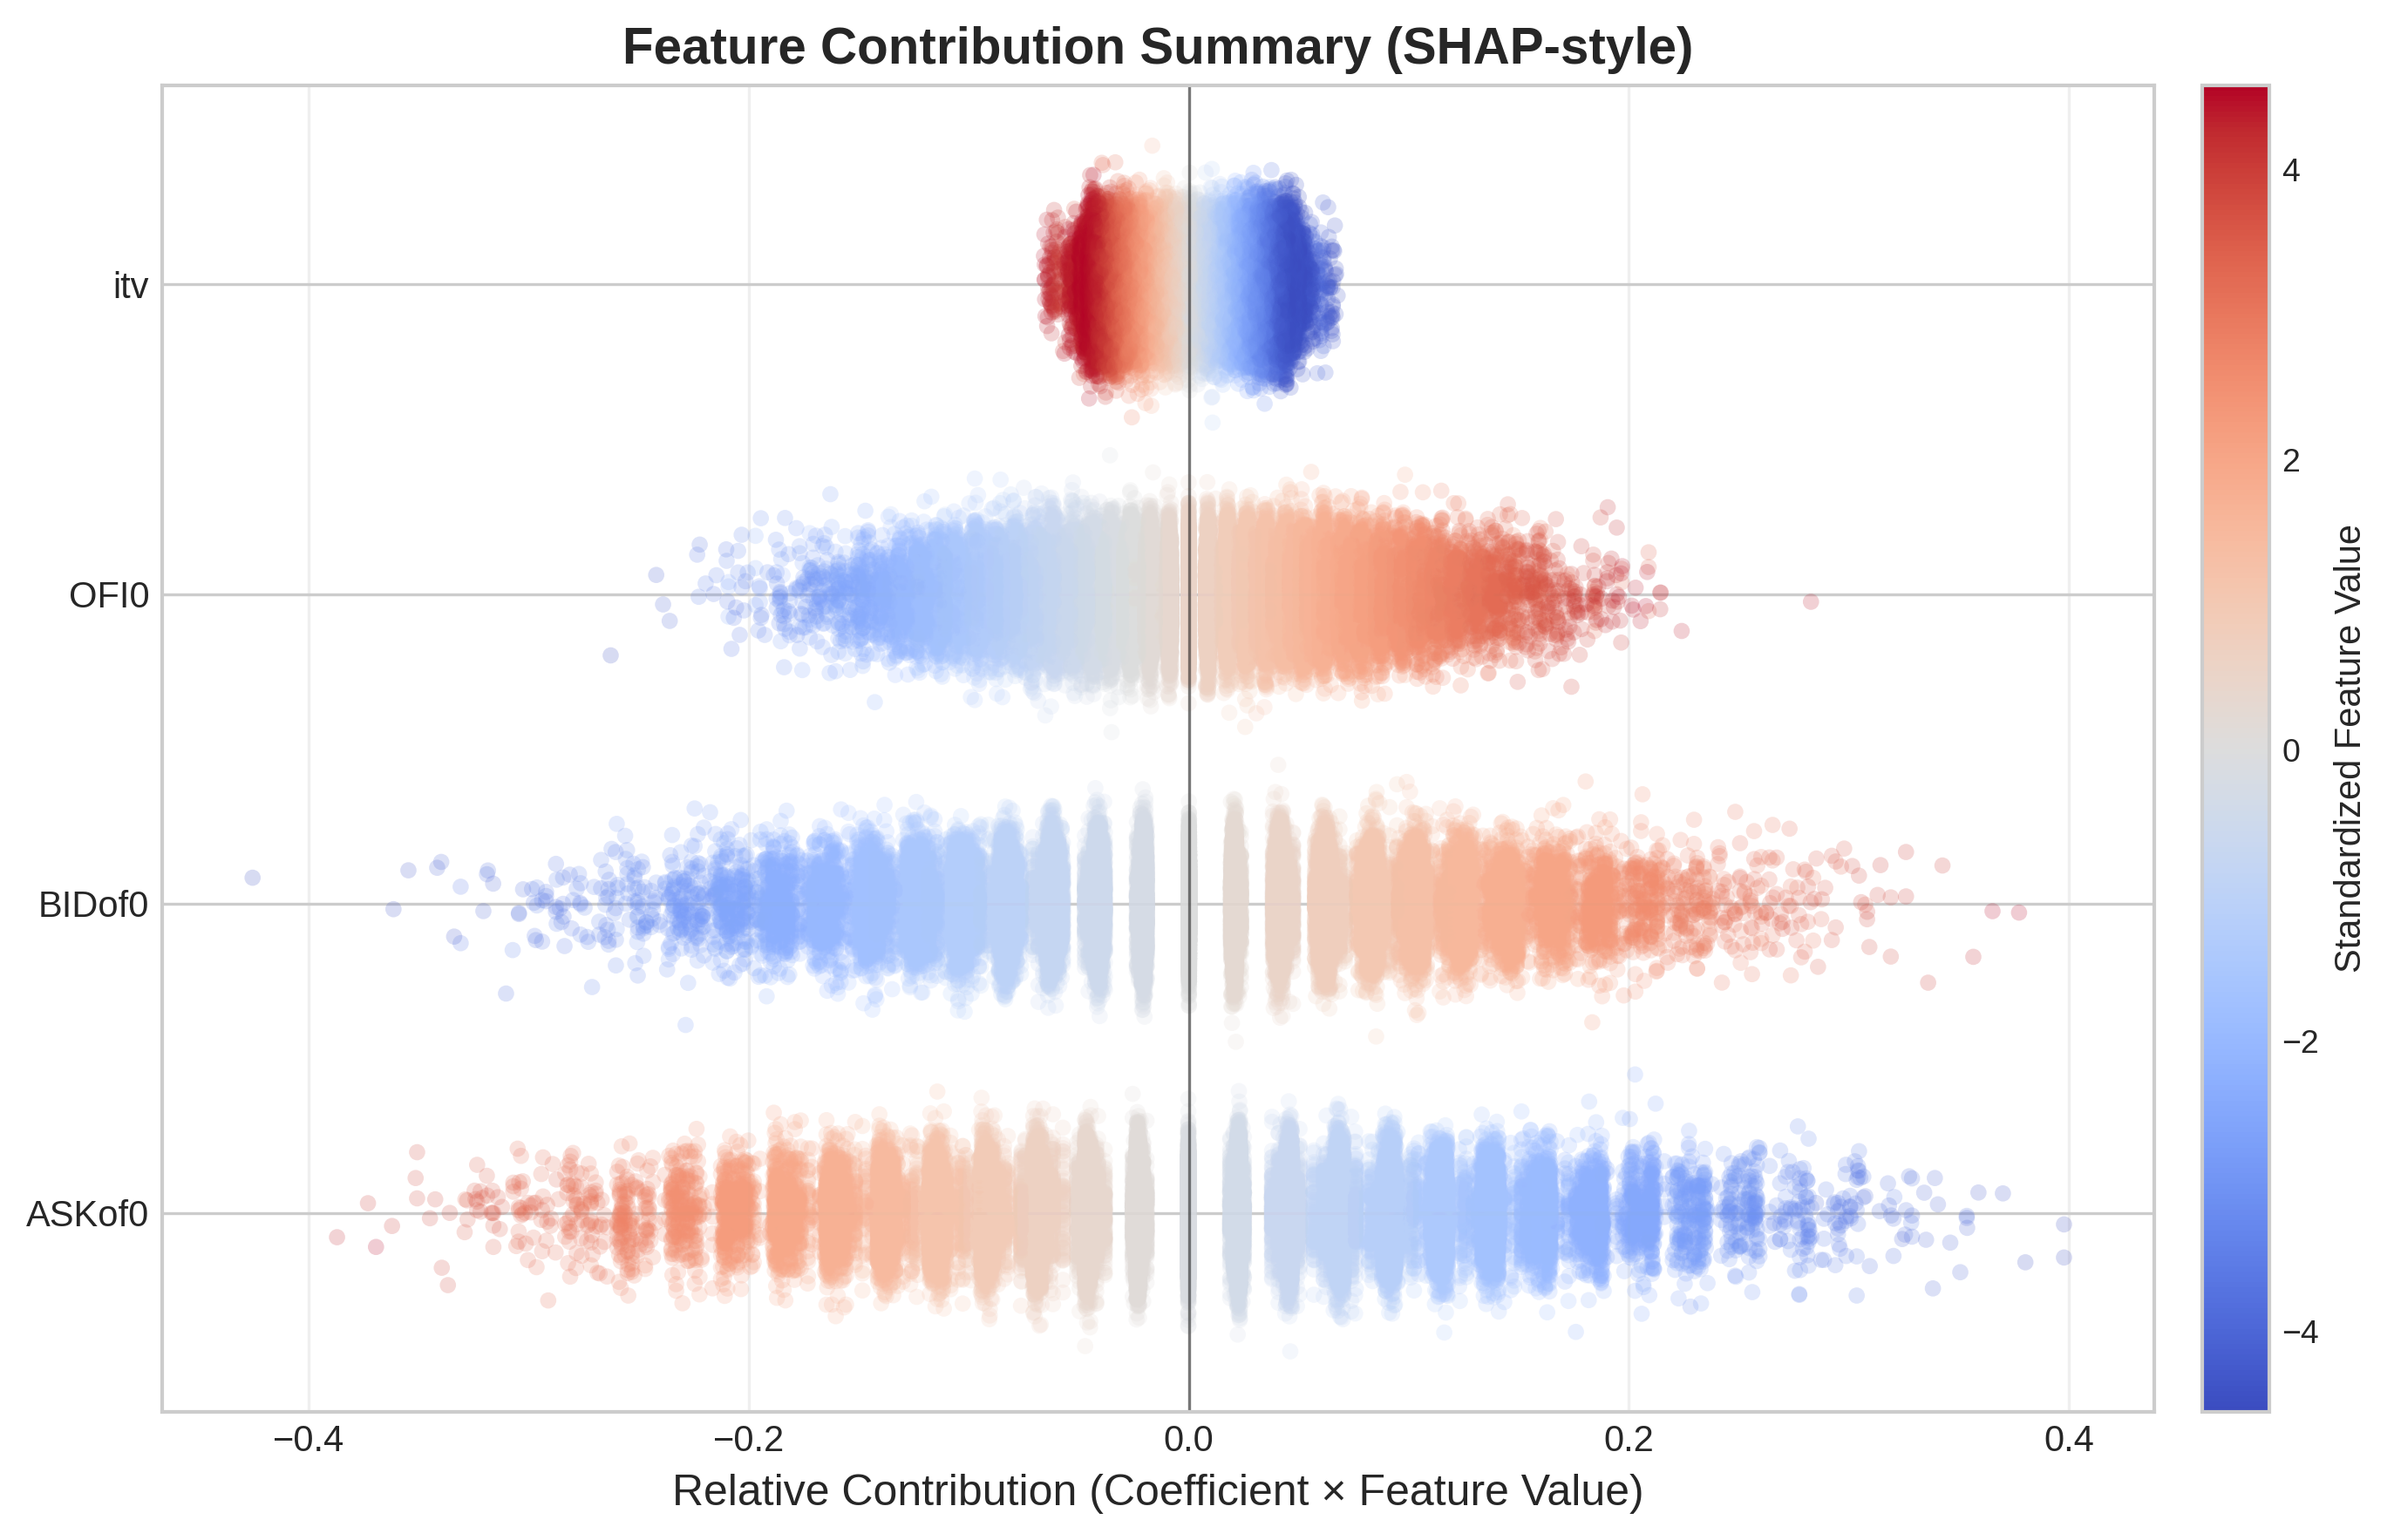
\includegraphics[width=\linewidth]{shap_summary_SA_03_synthetic_data.png}
  \caption{ARMAX–GARCH-DeepLOB SHAP scores \texttt{SA\_03}. The figure plots the product of the coefficient and the feature value for each sample.}
  \label{fig:shap_scores_sa_03}
\end{figure}

\begin{figure}[htb]
  \centering
  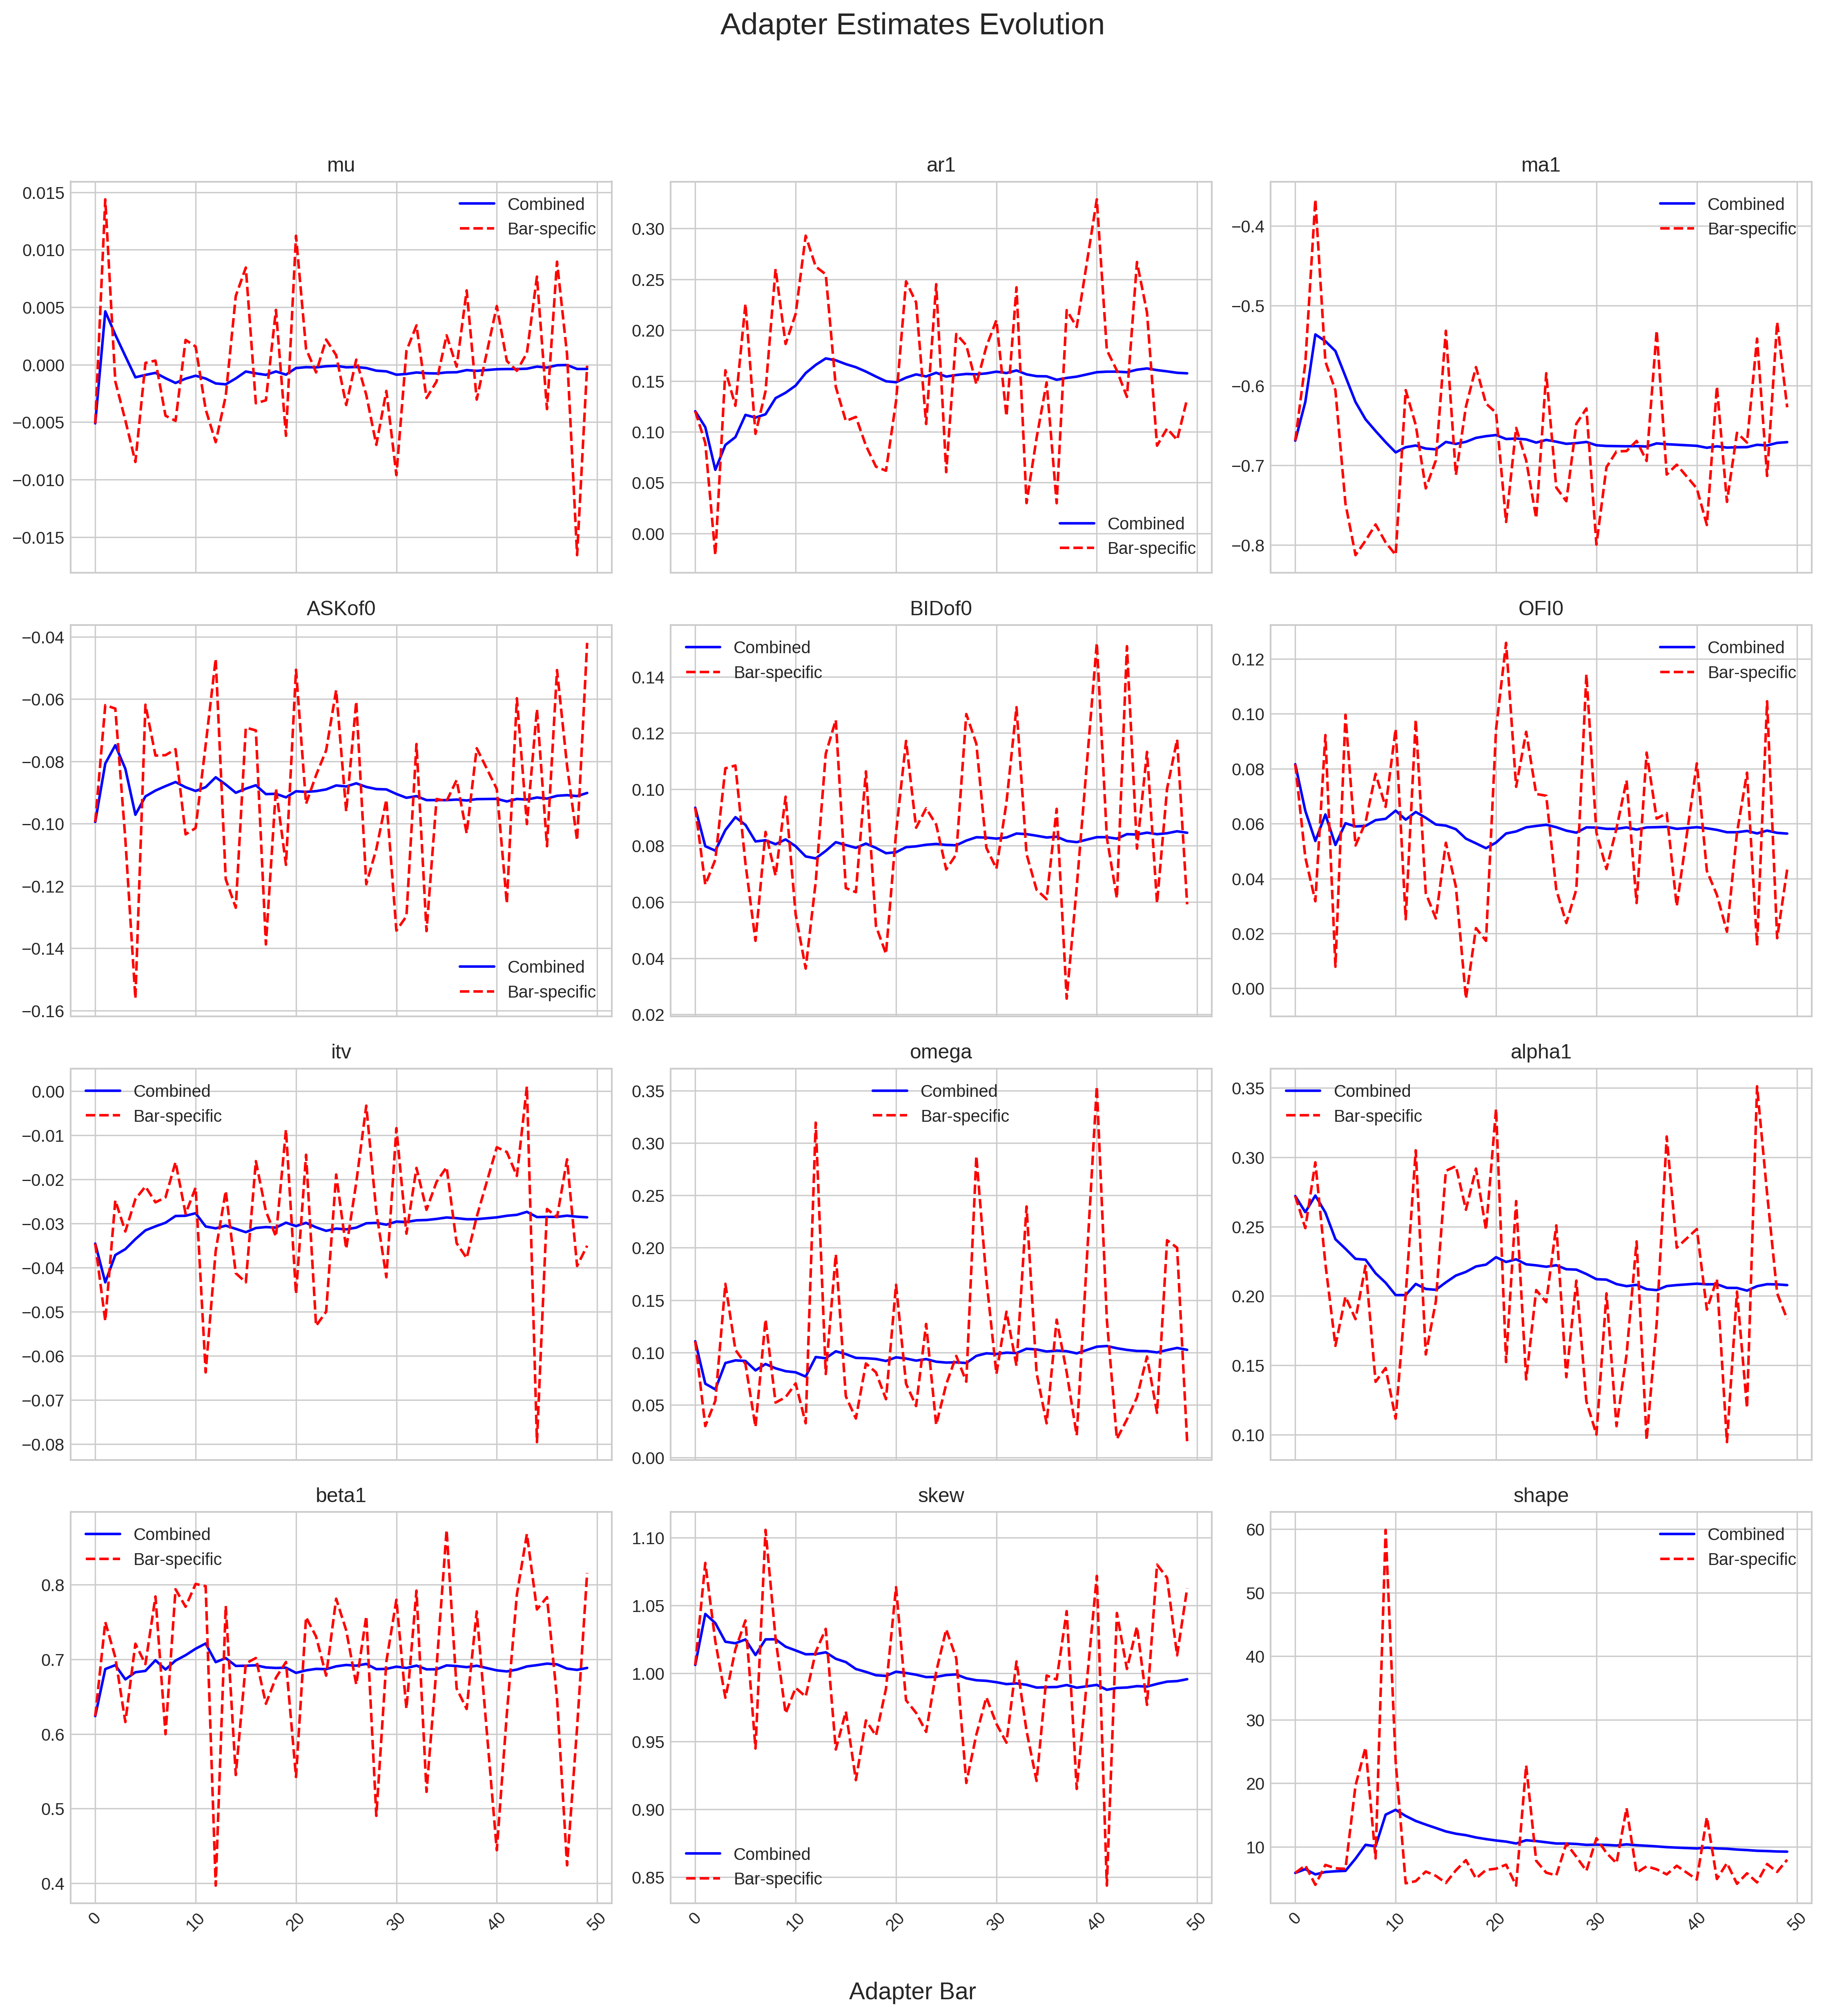
\includegraphics[width=\linewidth]{param_series_SA_03_synthetic_data.png}
  \caption{Evolution of parameter estimates for configuration \texttt{SA\_03}. Blue lines denote combined estimates, while red dashed lines denote bar-specific estimates across adapter bars.}
  \label{fig:param_series_sa_03}
\end{figure}


\begin{longtable}{@{}lll@{}}
\caption{Base configuration used in the experiments with market data.} 
\label{tab:base_config_market_data} \\
\toprule
\textbf{Category} & \textbf{Parameter} & \textbf{Value} \\ \midrule
\endfirsthead

\multicolumn{3}{c}%
{{\bfseries Table \thetable\ (continued)}} \\
\toprule
\textbf{Category} & \textbf{Parameter} & \textbf{Value} \\ \midrule
\endhead

\bottomrule
\endfoot

\multirow{8}{*}{General} 
 & Ticker & INTC \\
 & $\Delta^B$ & $7{,}200.0$ sec \\
 & $\Delta^A$ & $600.0$ sec \\
 & $\delta$ & $2.0$ sec \\
 & Seed & One per date pair \\
 & Session start & 9:45 AM EST \\
 & Session finish & 3:45 PM EST \\
 & Target Variable & $r^w$ \\ \midrule

\multirow{10}{*}{Backbone} 
 & Training Epochs & 10 \\
 & Batch size & 32 \\
 & Validation proportion & 0.1 \\
 & Buffer proportion & 0.05 \\
 & Windsorization quantile & 0.005 \\
 & ADF rejection threshold & 0.8 \\
 & KPSS verification threshold & 0.2 \\
 & NA threshold & 0.2 \\
 & Learning rate & 0.0001 \\
 & Correlation threshold & 0.95 \\ \midrule

\multirow{9}{*}{Interface} 
 & $\alpha$  & \{0.0, 0.1, 0.25, 0.5, 0.75, 0.9, 1.0\} \\
 & $\lambda_1$ & $\mathrm{logspace}(-4,1,25)$ \\
 & $\tau$   & \{0.25, 0.5, 1.0, 1.5, 2.0\} \\
 & $\lambda_2$ & $\mathrm{logspace}(0,1,25)$ \\
 & Validation proportion & 0.2 \\
 & Selection threshold & 0.29 ($L = 12$, $\alpha = 0.00005$) \\
 & Tolerance threshold & $10^{-6}$ \\
 & OLS significance level & 0.05 \\
 & Surrogate model lags & 5 \\ \midrule

\multirow{3}{*}{Adapter} 
 & ARMA order & (0,1) \\
 & \textbf{EGARCH} order & (1,1) \\
 & Error distribution & Negative Inverse Gaussian \\ 
 & Update Rule & Exponential Smoothing \\
\end{longtable}

% Add this to your preamble:
% \usepackage{longtable}

\begingroup
\small % Reduces font size slightly to ensure width fits
\setlength{\tabcolsep}{3pt} % Reduces space between columns
\begin{longtable}{@{}ccccccccc@{}}

% --- CAPTION AND LABEL ---
\caption{RelMAE-based overall rankings and average RelMAE values for each TTSTL configuration across the backbone bars in the INTC MBO dataset. DP denotes the date pair, UR the update rule, CC the covariate configuration, Rank BBX the overall ranking within backbone bar X, and RelMAE BBX the corresponding average forecasting error.} 
\label{tab:intc_data_results} \\

% --- HEADER FOR FIRST PAGE ---
\toprule
DP & UR & CC & Rank BB0 & RelMAE BB0 & Rank BB1 & RelMAE BB1 & Rank BB2 & RelMAE BB2 \\
\midrule
\endfirsthead

% --- HEADER FOR SUBSEQUENT PAGES ---
\multicolumn{9}{c}{{\bfseries \tablename\ \thetable{} -- continued from previous page}} \\
\toprule
DP & UR & CC & Rank BB0 & RelMAE BB1 & Rank BB1 & RelMAE BB2 & Rank BB3 & RelMAE BB2 \\
\midrule
\endhead

% --- FOOTER FOR BOTTOM OF PAGES ---
\midrule
\multicolumn{9}{r}{{Continued on next page}} \\
\bottomrule
\endfoot

% --- FOOTER FOR LAST PAGE ---
\bottomrule
\endlastfoot

% --- DATA CONTENT ---
1 & ES010 & 01 & 3.0 & 99.98\% & 3.0 & 100.63\% & 3.0 & 99.17\% \\
1 & ES010 & 02 & 3.0 & 99.98\% & 3.0 & 100.63\% & 3.0 & 99.17\% \\
1 & ES010 & 03 & 3.0 & 99.98\% & 3.0 & 100.63\% & 3.0 & 99.17\% \\
1 & ES010 & 04 & 3.0 & 99.98\% & 3.0 & 100.63\% & 3.0 & 99.17\% \\
1 & ES010 & 05 & 6.0 & 100.02\% & 6.0 & 100.75\% & 6.0 & 99.20\% \\
1 & ES010 & 06 & 3.0 & 99.98\% & 3.0 & 100.63\% & 3.0 & 99.17\% \\
2 & ES010 & 01 & 3.0 & 99.84\% & 3.0 & 100.56\% & 4.0 & 100.39\% \\
2 & ES010 & 02 & 3.0 & 99.84\% & 3.0 & 100.56\% & 4.0 & 100.39\% \\
2 & ES010 & 03 & 3.0 & 99.84\% & 3.0 & 100.56\% & 4.0 & 100.39\% \\
2 & ES010 & 04 & 3.0 & 99.84\% & 3.0 & 100.56\% & 4.0 & 100.39\% \\
2 & ES010 & 05 & 6.0 & 100.43\% & 6.0 & 100.75\% & 1.0 & 100.32\% \\
2 & ES010 & 06 & 3.0 & 99.84\% & 3.0 & 100.56\% & 4.0 & 100.39\% \\
3 & ES010 & 01 & 3.0 & 99.85\% & 3.0 & 100.17\% & 2.5 & 100.53\% \\
3 & ES010 & 02 & 3.0 & 99.85\% & 3.0 & 100.17\% & 5.5 & 100.59\% \\
3 & ES010 & 03 & 3.0 & 99.85\% & 3.0 & 100.17\% & 2.5 & 100.53\% \\
3 & ES010 & 04 & 3.0 & 99.85\% & 3.0 & 100.17\% & 2.5 & 100.53\% \\
3 & ES010 & 05 & 6.0 & 99.91\% & 6.0 & 100.32\% & 5.5 & 100.59\% \\
3 & ES010 & 06 & 3.0 & 99.85\% & 3.0 & 100.17\% & 2.5 & 100.53\% \\
4 & ES010 & 01 & 3.0 & 99.64\% & 4.5 & 102.53\% & 4.0 & 101.48\% \\
4 & ES010 & 02 & 3.0 & 99.64\% & 1.5 & 101.04\% & 4.0 & 101.48\% \\
4 & ES010 & 03 & 3.0 & 99.64\% & 4.5 & 102.53\% & 4.0 & 101.48\% \\
4 & ES010 & 04 & 3.0 & 99.64\% & 4.5 & 102.53\% & 4.0 & 101.48\% \\
4 & ES010 & 05 & 6.0 & 100.45\% & 1.5 & 101.04\% & 1.0 & 101.38\% \\
4 & ES010 & 06 & 3.0 & 99.64\% & 4.5 & 102.53\% & 4.0 & 101.48\% \\
5 & ES010 & 01 & 3.0 & 99.93\% & 4.5 & 99.80\% & 4.0 & 99.77\% \\
5 & ES010 & 02 & 3.0 & 99.93\% & 1.5 & 99.76\% & 4.0 & 99.77\% \\
5 & ES010 & 03 & 3.0 & 99.93\% & 4.5 & 99.80\% & 4.0 & 99.77\% \\
5 & ES010 & 04 & 3.0 & 99.93\% & 4.5 & 99.80\% & 4.0 & 99.77\% \\
5 & ES010 & 05 & 6.0 & 100.06\% & 1.5 & 99.76\% & 1.0 & 99.77\% \\
5 & ES010 & 06 & 3.0 & 99.93\% & 4.5 & 99.80\% & 4.0 & 99.77\% \\
6 & ES010 & 01 & 4.0 & 100.40\% & 3.5 & 102.23\% & 2.5 & 100.14\% \\
6 & ES010 & 02 & 4.0 & 100.40\% & 5.5 & 131.02\% & 5.5 & 127.17\% \\
6 & ES010 & 03 & 4.0 & 100.40\% & 1.5 & 100.67\% & 2.5 & 100.14\% \\
6 & ES010 & 04 & 4.0 & 100.40\% & 3.5 & 102.23\% & 2.5 & 100.14\% \\
6 & ES010 & 05 & 1.0 & 100.36\% & 5.5 & 131.02\% & 5.5 & 127.17\% \\
6 & ES010 & 06 & 4.0 & 100.40\% & 1.5 & 100.67\% & 2.5 & 100.14\% \\
7 & ES010 & 01 & 3.0 & 99.99\% & 2.5 & 99.00\% & 3.0 & 99.26\% \\
7 & ES010 & 02 & 3.0 & 99.99\% & 5.5 & 112.60\% & 3.0 & 99.26\% \\
7 & ES010 & 03 & 3.0 & 99.99\% & 2.5 & 99.00\% & 3.0 & 99.26\% \\
7 & ES010 & 04 & 3.0 & 99.99\% & 2.5 & 99.00\% & 3.0 & 99.26\% \\
7 & ES010 & 05 & 6.0 & 100.03\% & 5.5 & 112.60\% & 6.0 & 99.27\% \\
7 & ES010 & 06 & 3.0 & 99.99\% & 2.5 & 99.00\% & 3.0 & 99.26\% \\
8 & ES010 & 01 & 3.0 & 98.15\% & 4.0 & 101.29\% & 3.0 & 100.14\% \\
8 & ES010 & 02 & 3.0 & 98.15\% & 4.0 & 101.29\% & 3.0 & 100.14\% \\
8 & ES010 & 03 & 3.0 & 98.15\% & 4.0 & 101.29\% & 3.0 & 100.14\% \\
8 & ES010 & 04 & 3.0 & 98.15\% & 4.0 & 101.29\% & 3.0 & 100.14\% \\
8 & ES010 & 05 & 6.0 & 98.67\% & 1.0 & 100.88\% & 6.0 & 100.27\% \\
8 & ES010 & 06 & 3.0 & 98.15\% & 4.0 & 101.29\% & 3.0 & 100.14\% \\
9 & ES010 & 01 & 3.0 & 99.77\% & 2.5 & 100.34\% & 2.0 & 100.46\% \\
9 & ES010 & 02 & 3.0 & 99.77\% & 5.5 & 101.93\% & 5.0 & 100.56\% \\
9 & ES010 & 03 & 3.0 & 99.77\% & 2.5 & 100.34\% & 5.0 & 100.56\% \\
9 & ES010 & 04 & 3.0 & 99.77\% & 2.5 & 100.34\% & 1.0 & 100.46\% \\
9 & ES010 & 05 & 6.0 & 99.75\% & 5.5 & 101.93\% & 3.0 & 100.68\% \\
9 & ES010 & 06 & 3.0 & 99.77\% & 2.5 & 100.34\% & 5.0 & 100.56\% \\
10 & ES010 & 01 & 3.0 & 100.33\% & 3.0 & 100.57\% & 3.0 & 99.83\% \\
10 & ES010 & 02 & 3.0 & 100.33\% & 3.0 & 100.57\% & 3.0 & 99.83\% \\
10 & ES010 & 03 & 3.0 & 100.33\% & 3.0 & 100.57\% & 3.0 & 99.83\% \\
10 & ES010 & 04 & 3.0 & 100.33\% & 3.0 & 100.57\% & 3.0 & 99.83\% \\
10 & ES010 & 05 & 6.0 & 100.70\% & 6.0 & 100.59\% & 6.0 & 99.88\% \\
10 & ES010 & 06 & 3.0 & 100.33\% & 3.0 & 100.57\% & 3.0 & 99.83\% \\
\end{longtable}
\endgroup

\begin{figure}[ht!]
\centering

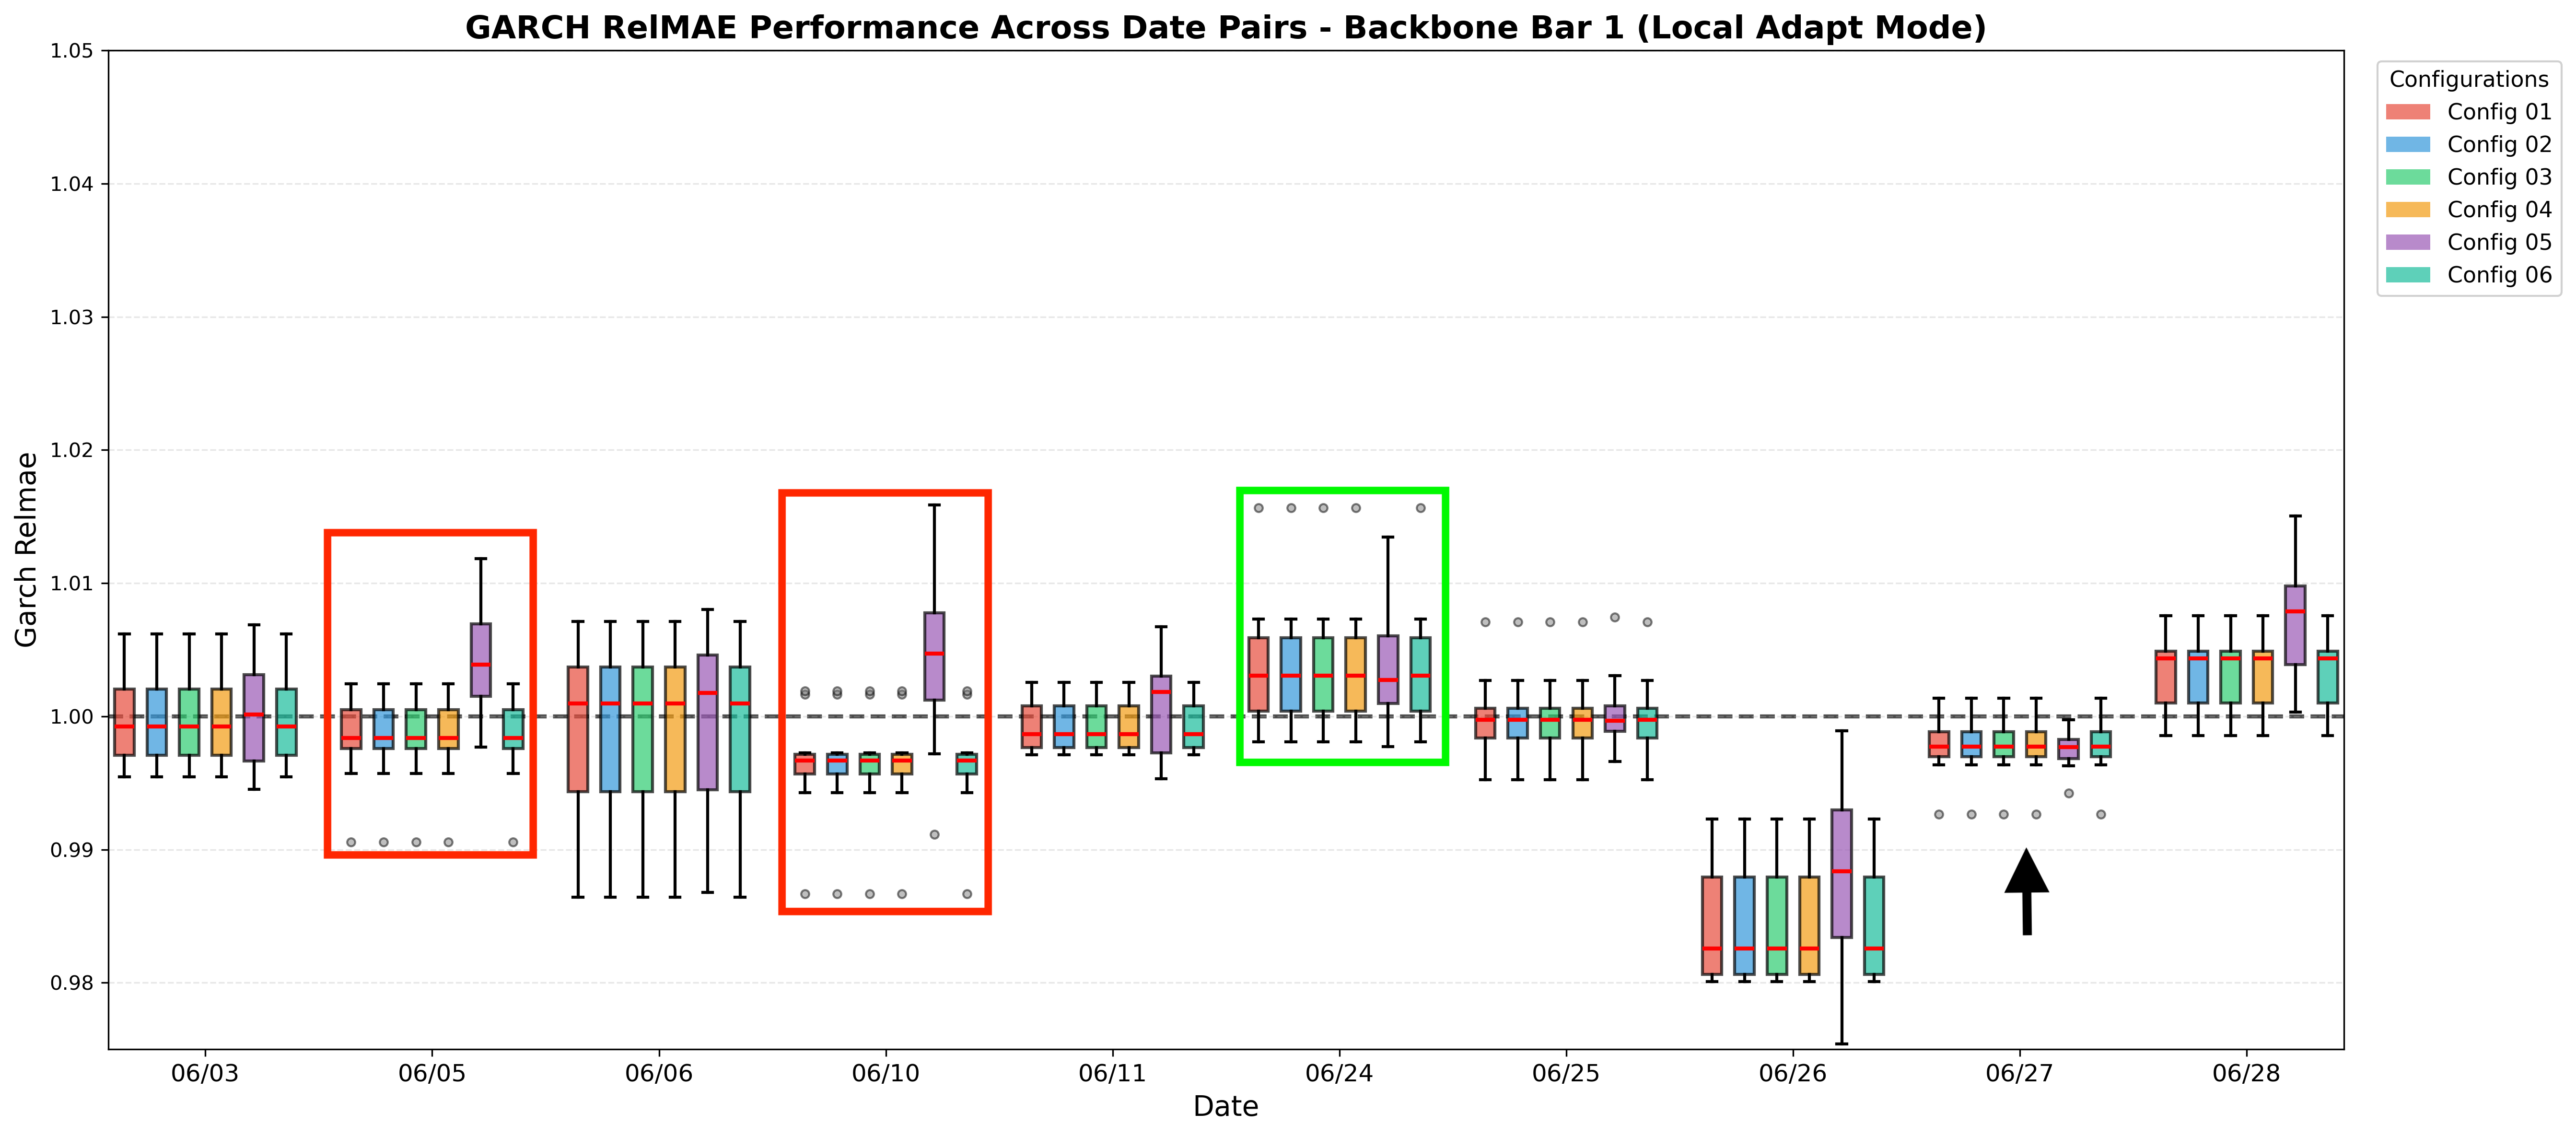
\includegraphics[width=0.9\linewidth]{sequential_boxplot_bb_000_marked.png}
\vspace{0.5em}
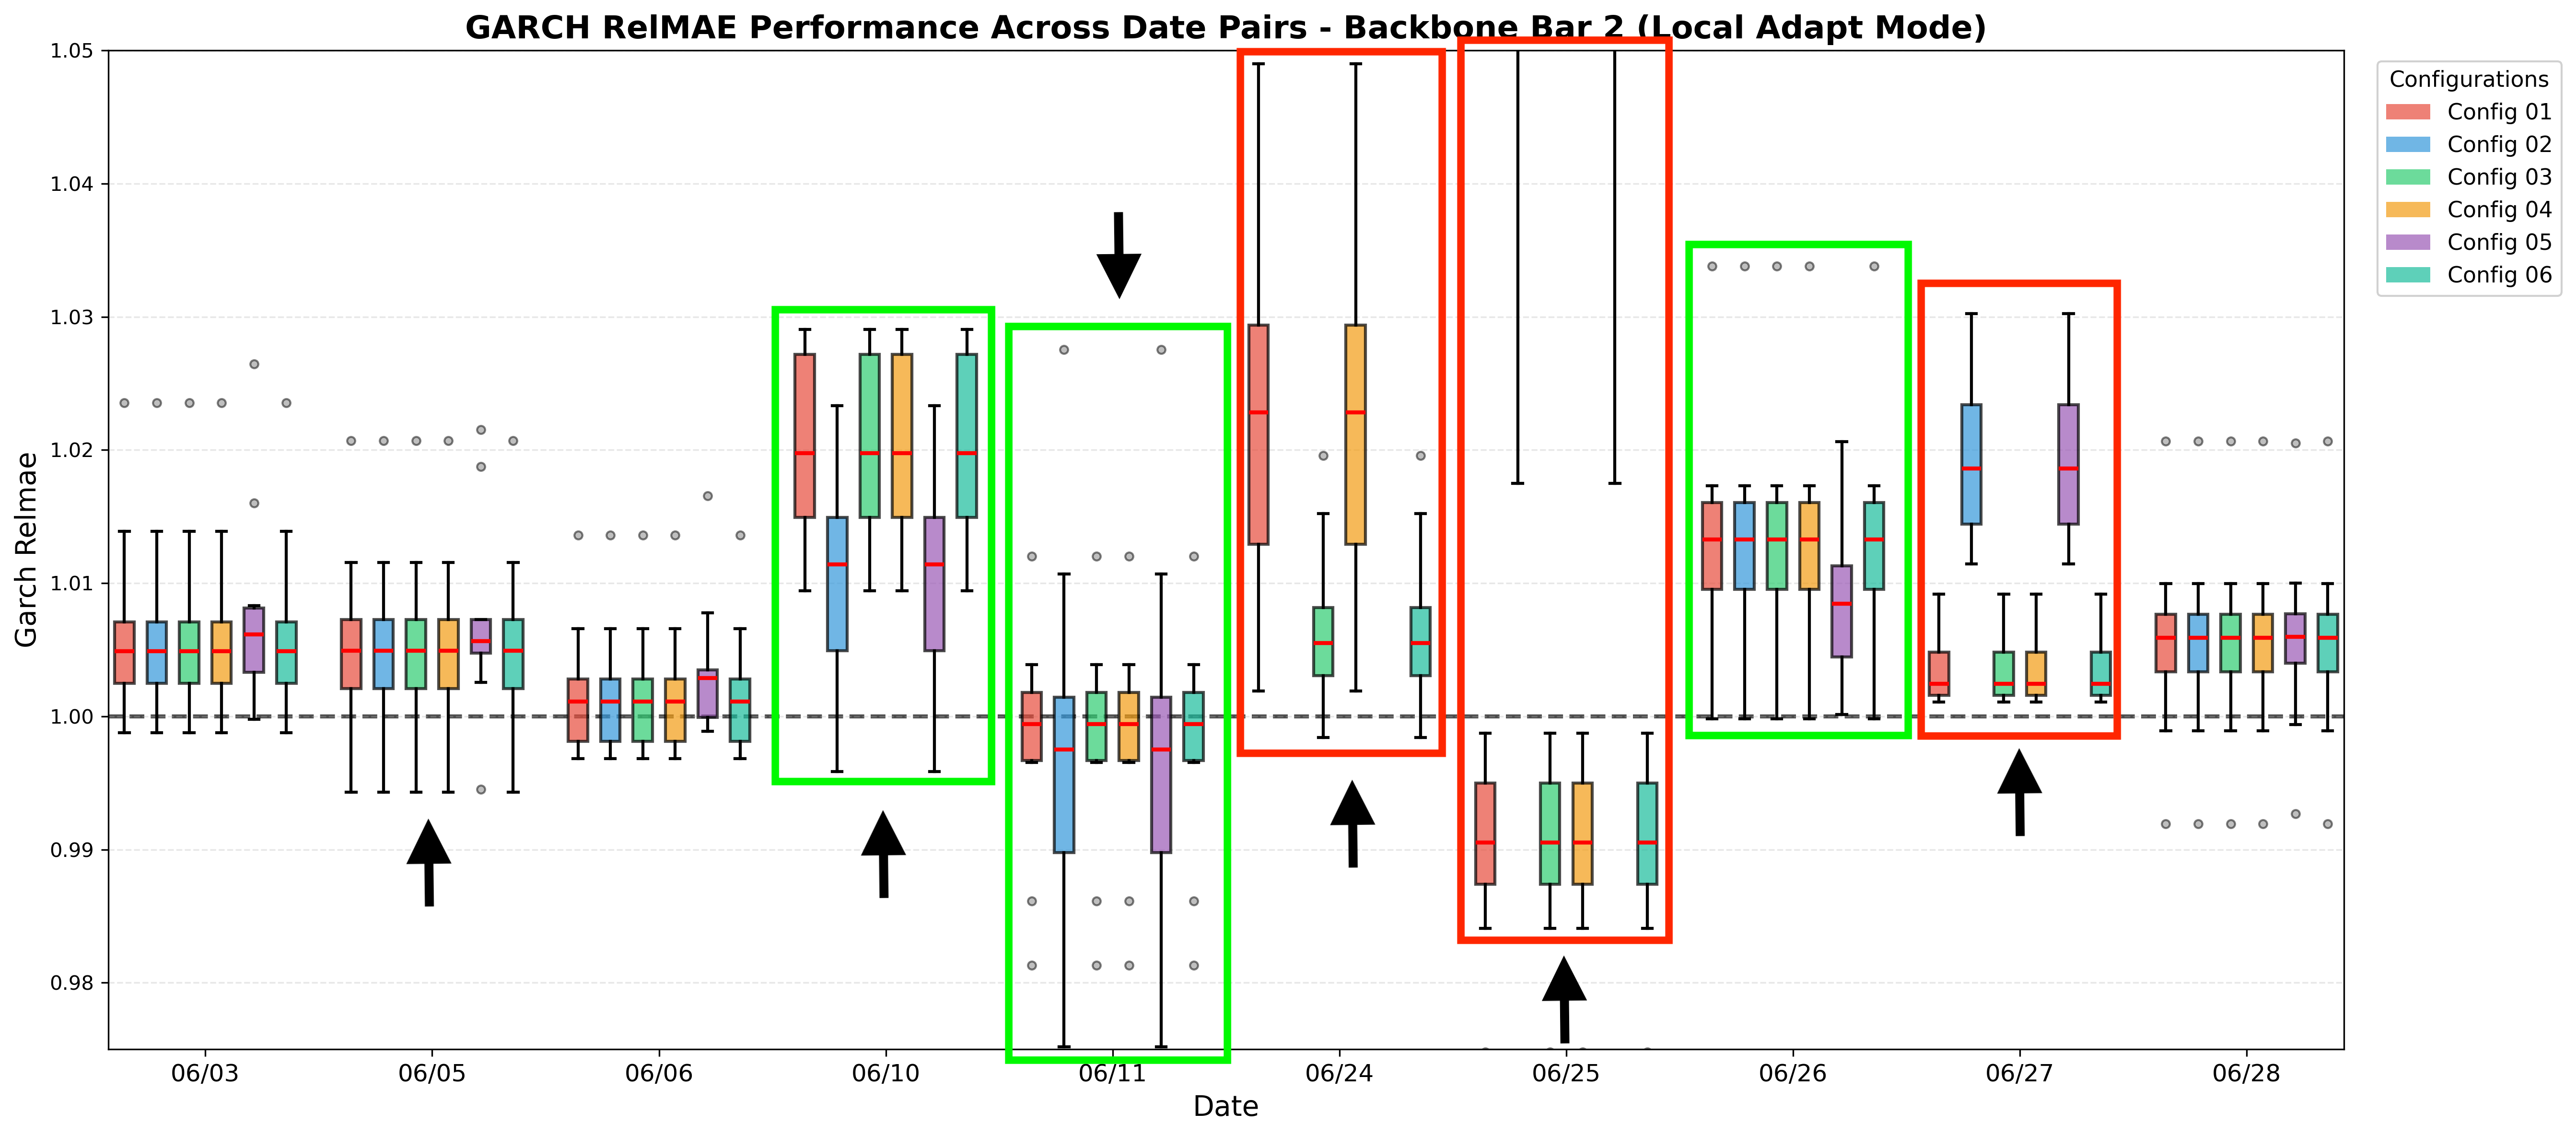
\includegraphics[width=0.9\linewidth]{sequential_boxplot_bb_001_marked.png}
\vspace{0.5em}
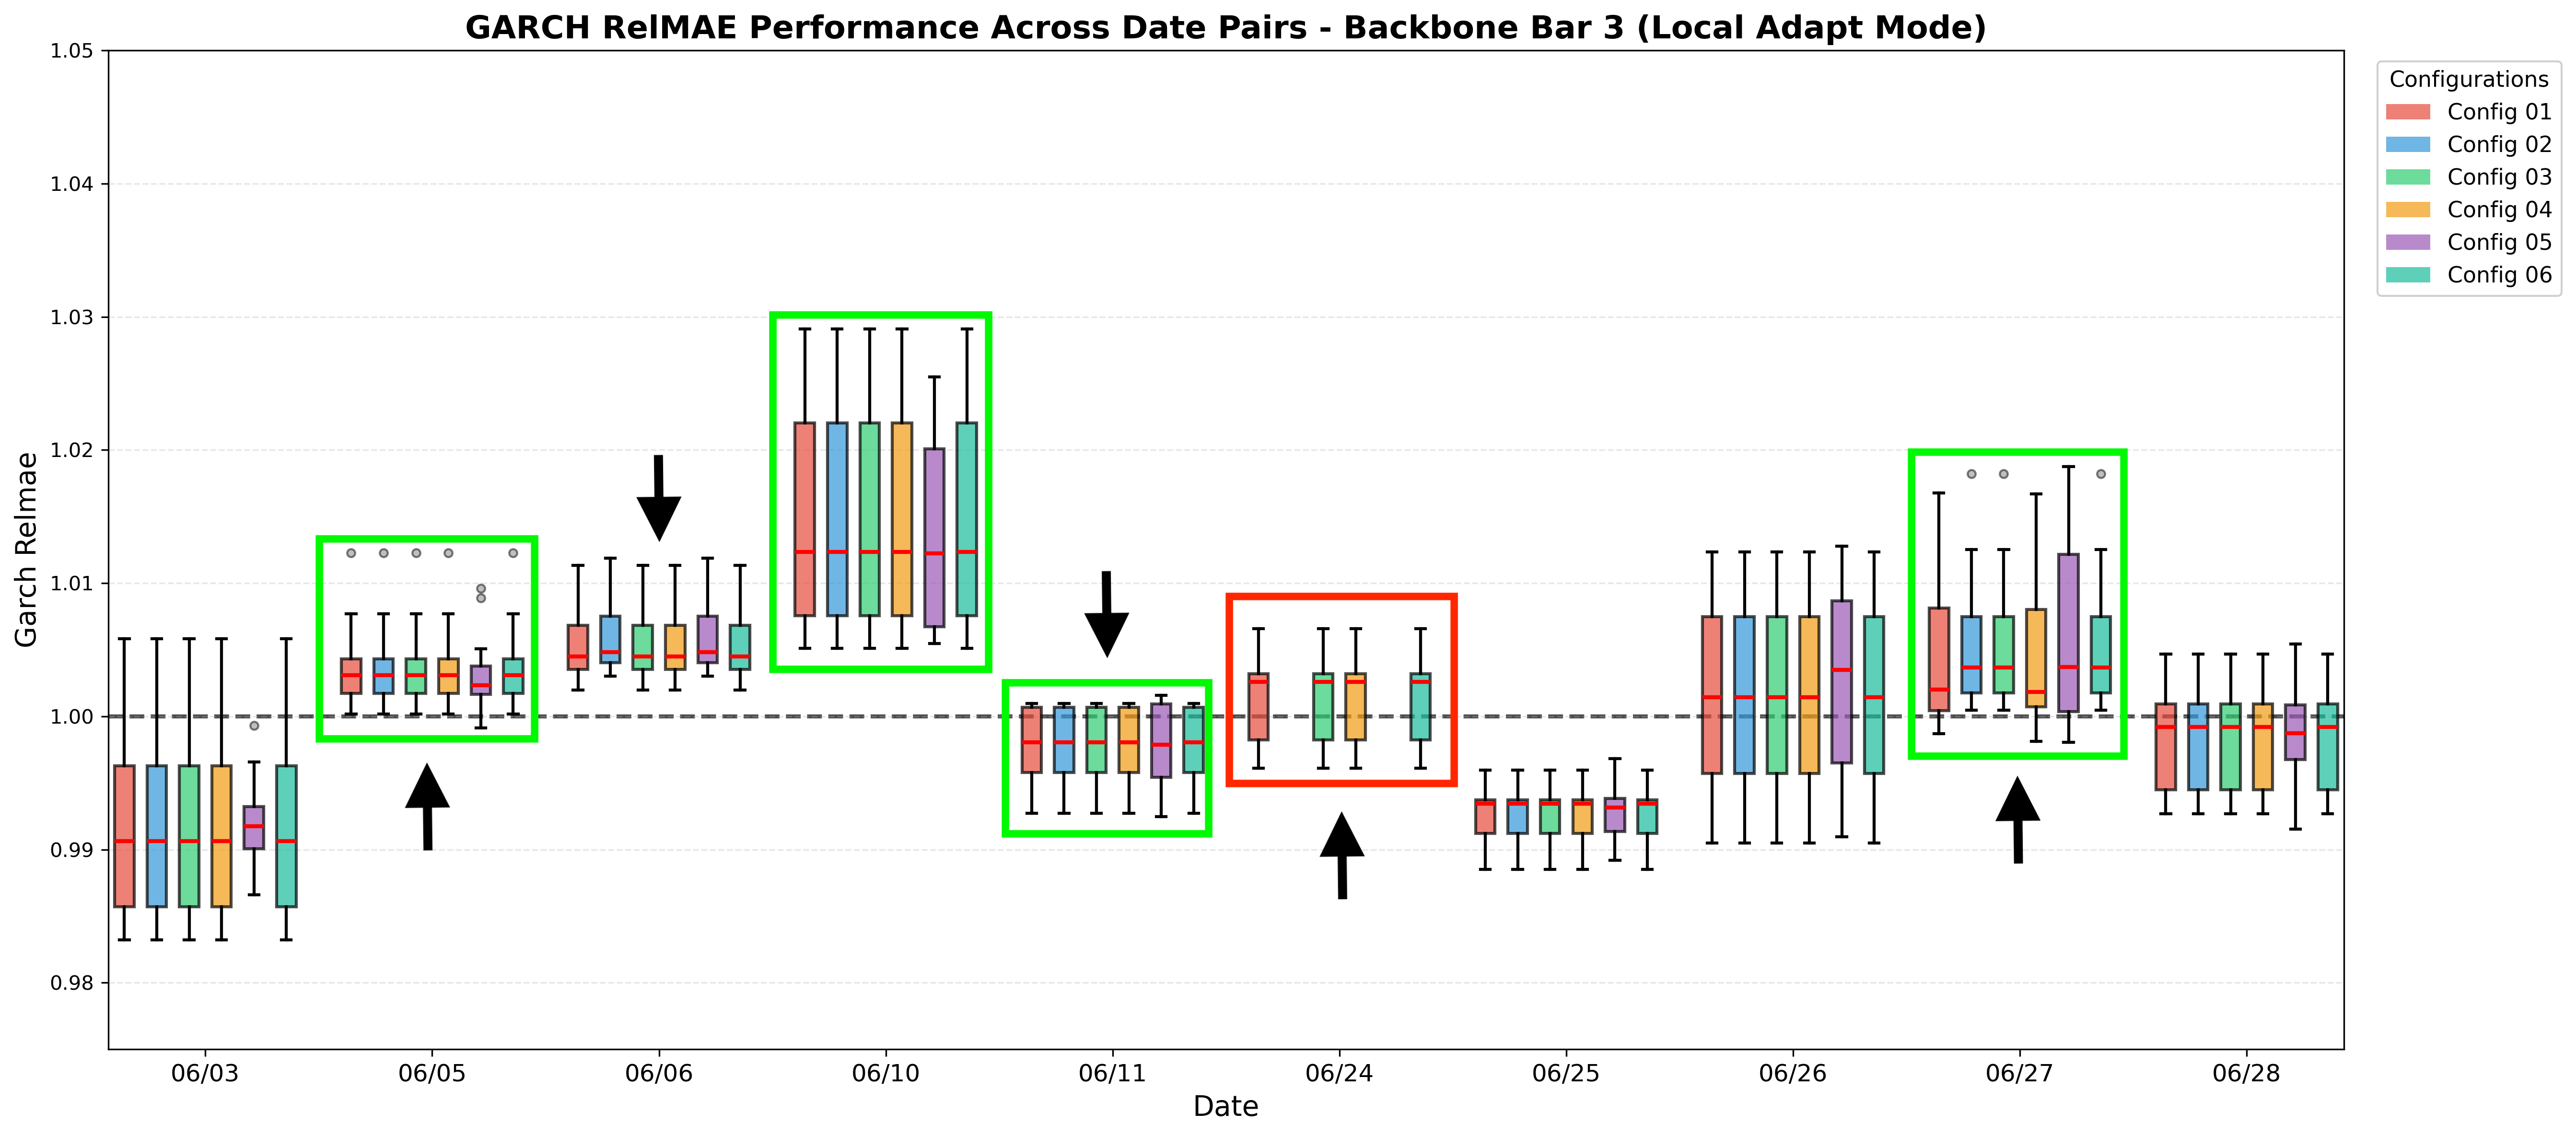
\includegraphics[width=0.9\linewidth]{sequential_boxplot_bb_002_marked.png}

\caption{Sequential RelMAE boxplots for the INTC dataset across date pairs in Local Adapt mode for Backbone Bar 1 (top), Backbone Bar 2 (middle), and Backbone Bar 3 (bottom). The horizontal dashed line at 1.00 represents the naive model baseline. Green rectangles highlight instances where covariate configurations \texttt{05} (raw CNN-LSTM output) or \texttt{01} (full configuration) outperformed configuration \texttt{06} (no covariates). Red rectangles indicate date pairs where configuration \texttt{05} exhibited significant underperformance. Black arrows mark backbone bars where the CNN-LSTM weights were updated during the preceding Global Retrain step. Note that the boxplots corresponding to configurations \texttt{02} and \texttt{05} of Backbone Bars 2 and 3 on 06/24, and Backbone Bar 2 on 06/27, lie above the superior margin.}
\label{fig:sequential_boxplot_intc_data}
\end{figure}

$r^w_j$ $\mathrm{CNNLSTM}_{\mathbf{W}}\!\left(\widetilde{\mathbf{OF}}^{\mathcal{P}^{(E)}}_{i_{t-1}-99:i_{t-1}}\right)$ $OFI_{0, j}$

\begin{figure}[ht!]
\centering
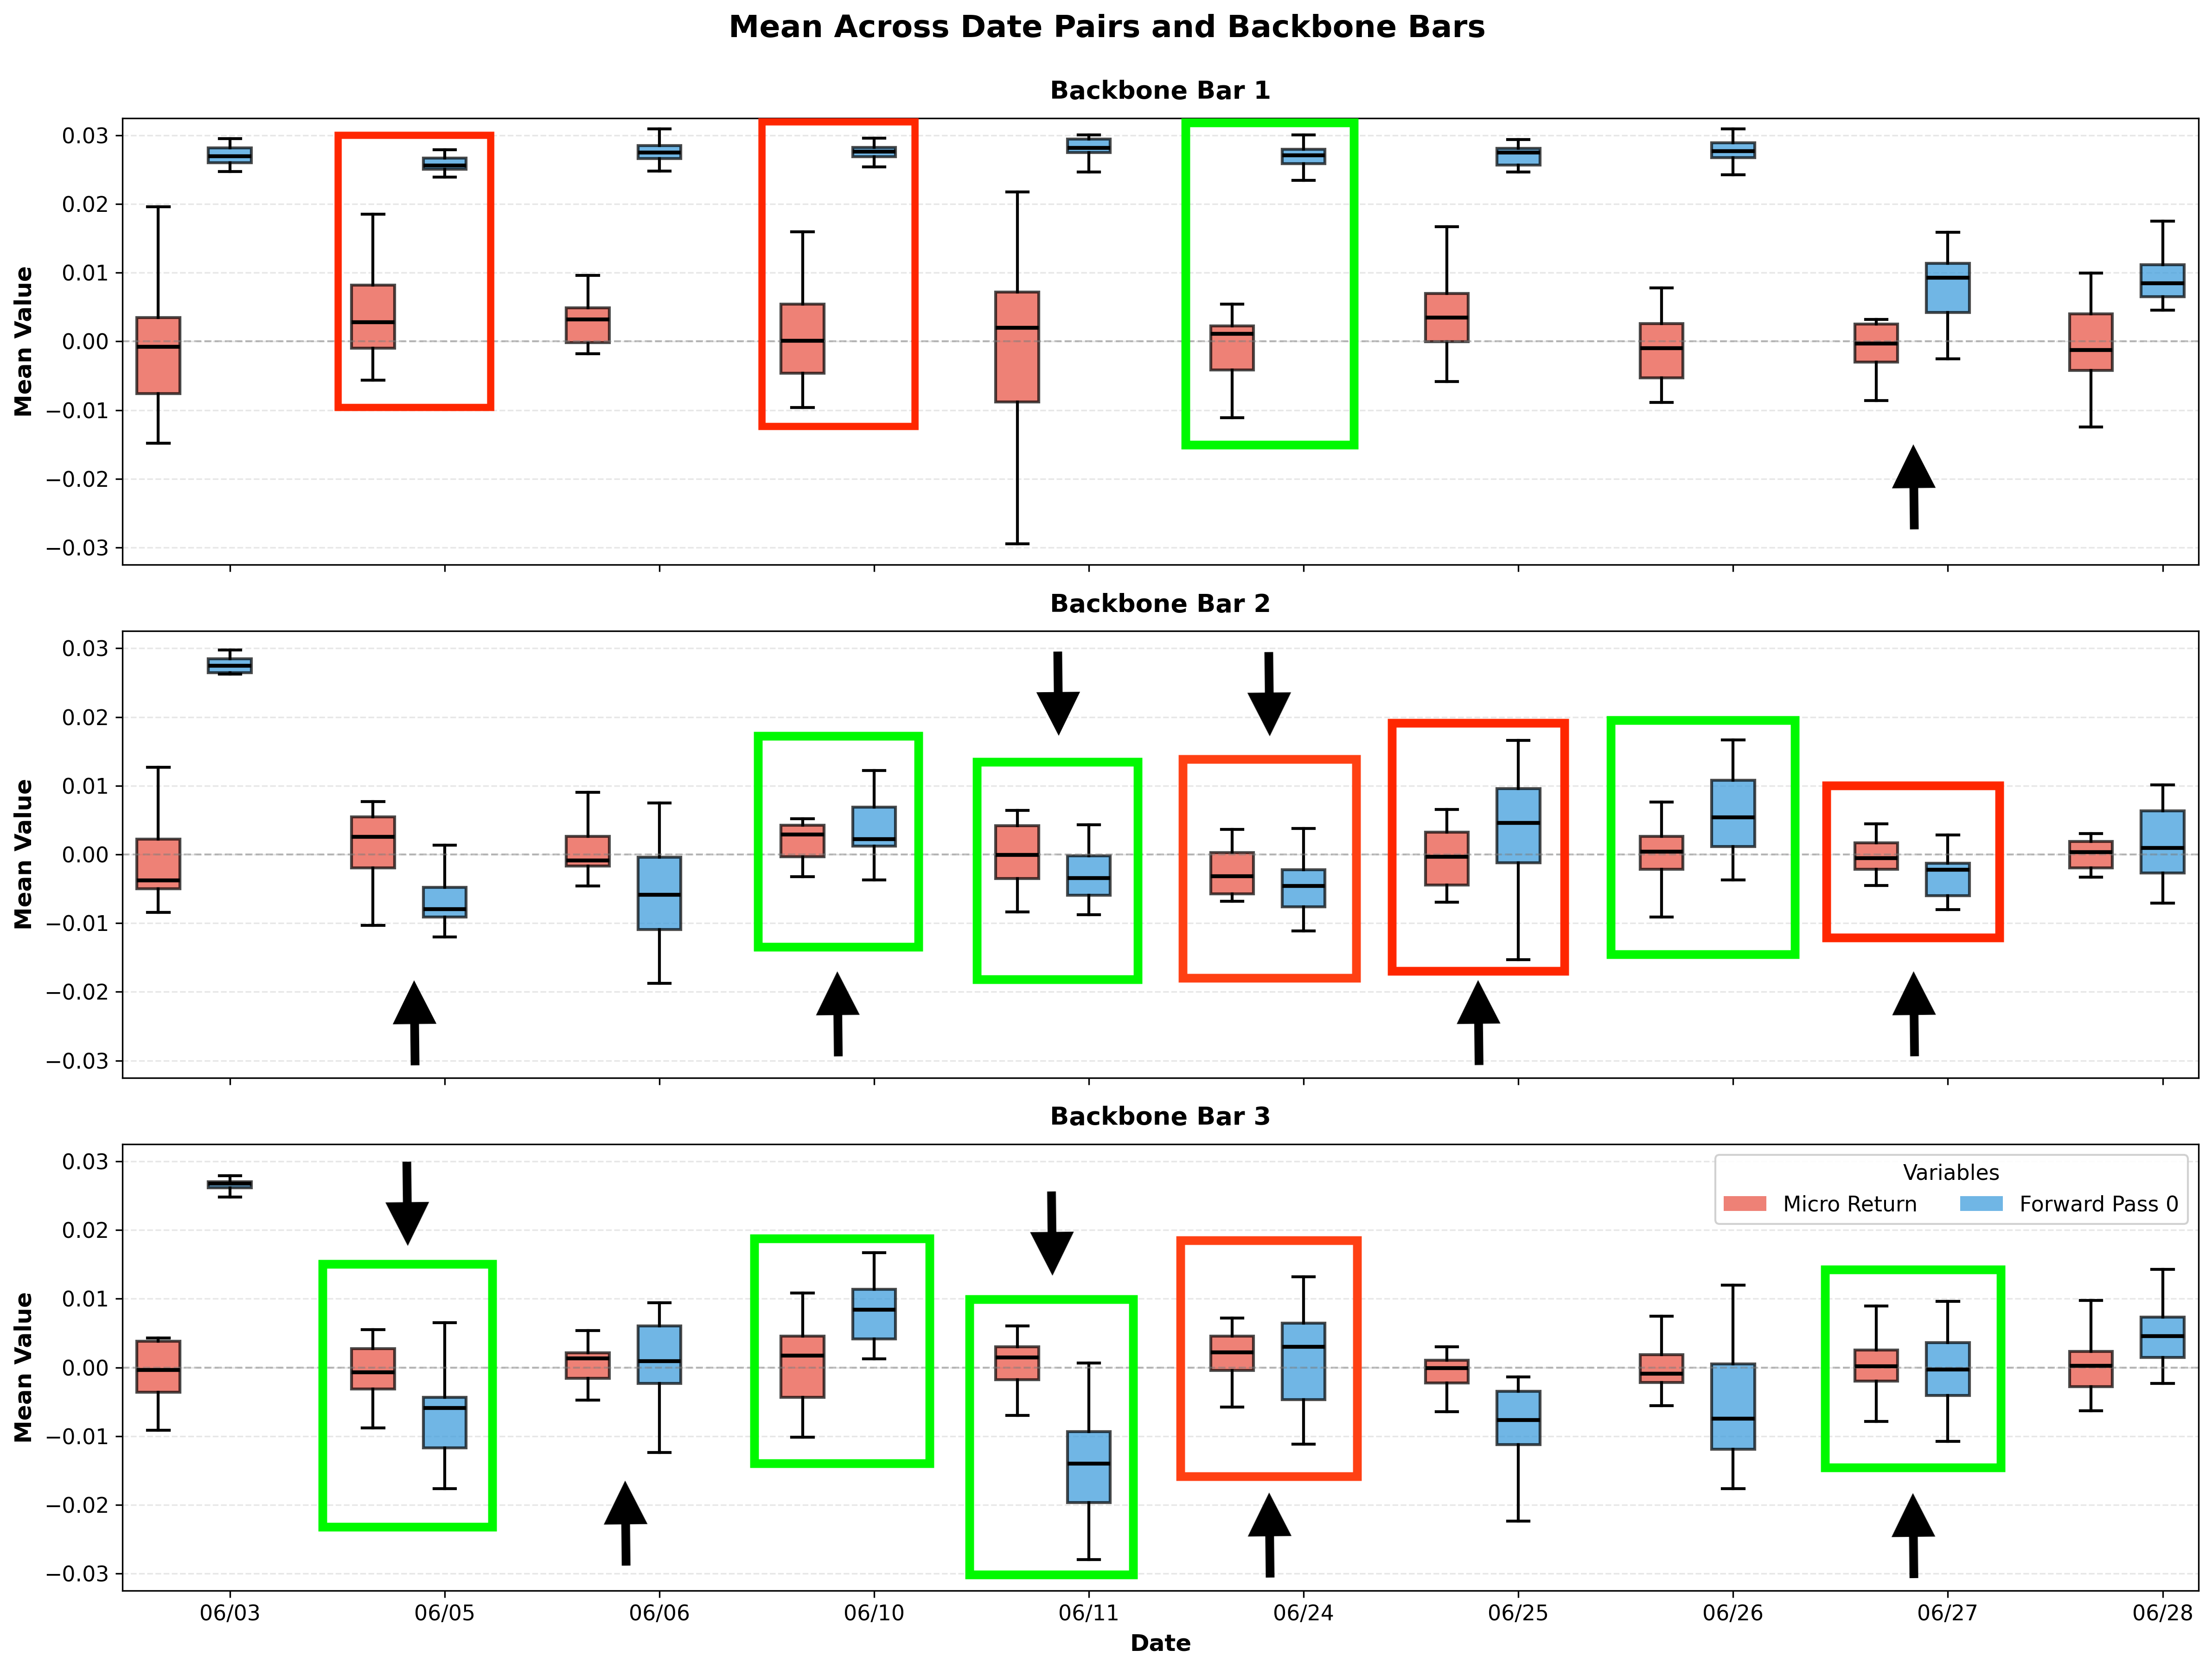
\includegraphics[width=0.9\linewidth]{covariate_aggregate_mean_boxplots_marked.png}
\caption{Distribution of the \textbf{mean} of the Micro-Return ($r^w_j$) and CNN-LSTM Output ($\mathrm{CNNLSTM}_{\mathbf{W}}\!\left(\widetilde{\mathbf{OF}}^{\mathcal{P}^{(E)}}_{i_{t-1}-99:i_{t-1}}\right)$) computed on each adapter bar and aggregated at the backbone bar level. See Figure~\ref{fig:sequential_boxplot_intc_data} for the interpretation of the markers.}
\label{fig:covariate_aggregate_mean}
\end{figure}

\begin{figure}[ht!]
\centering
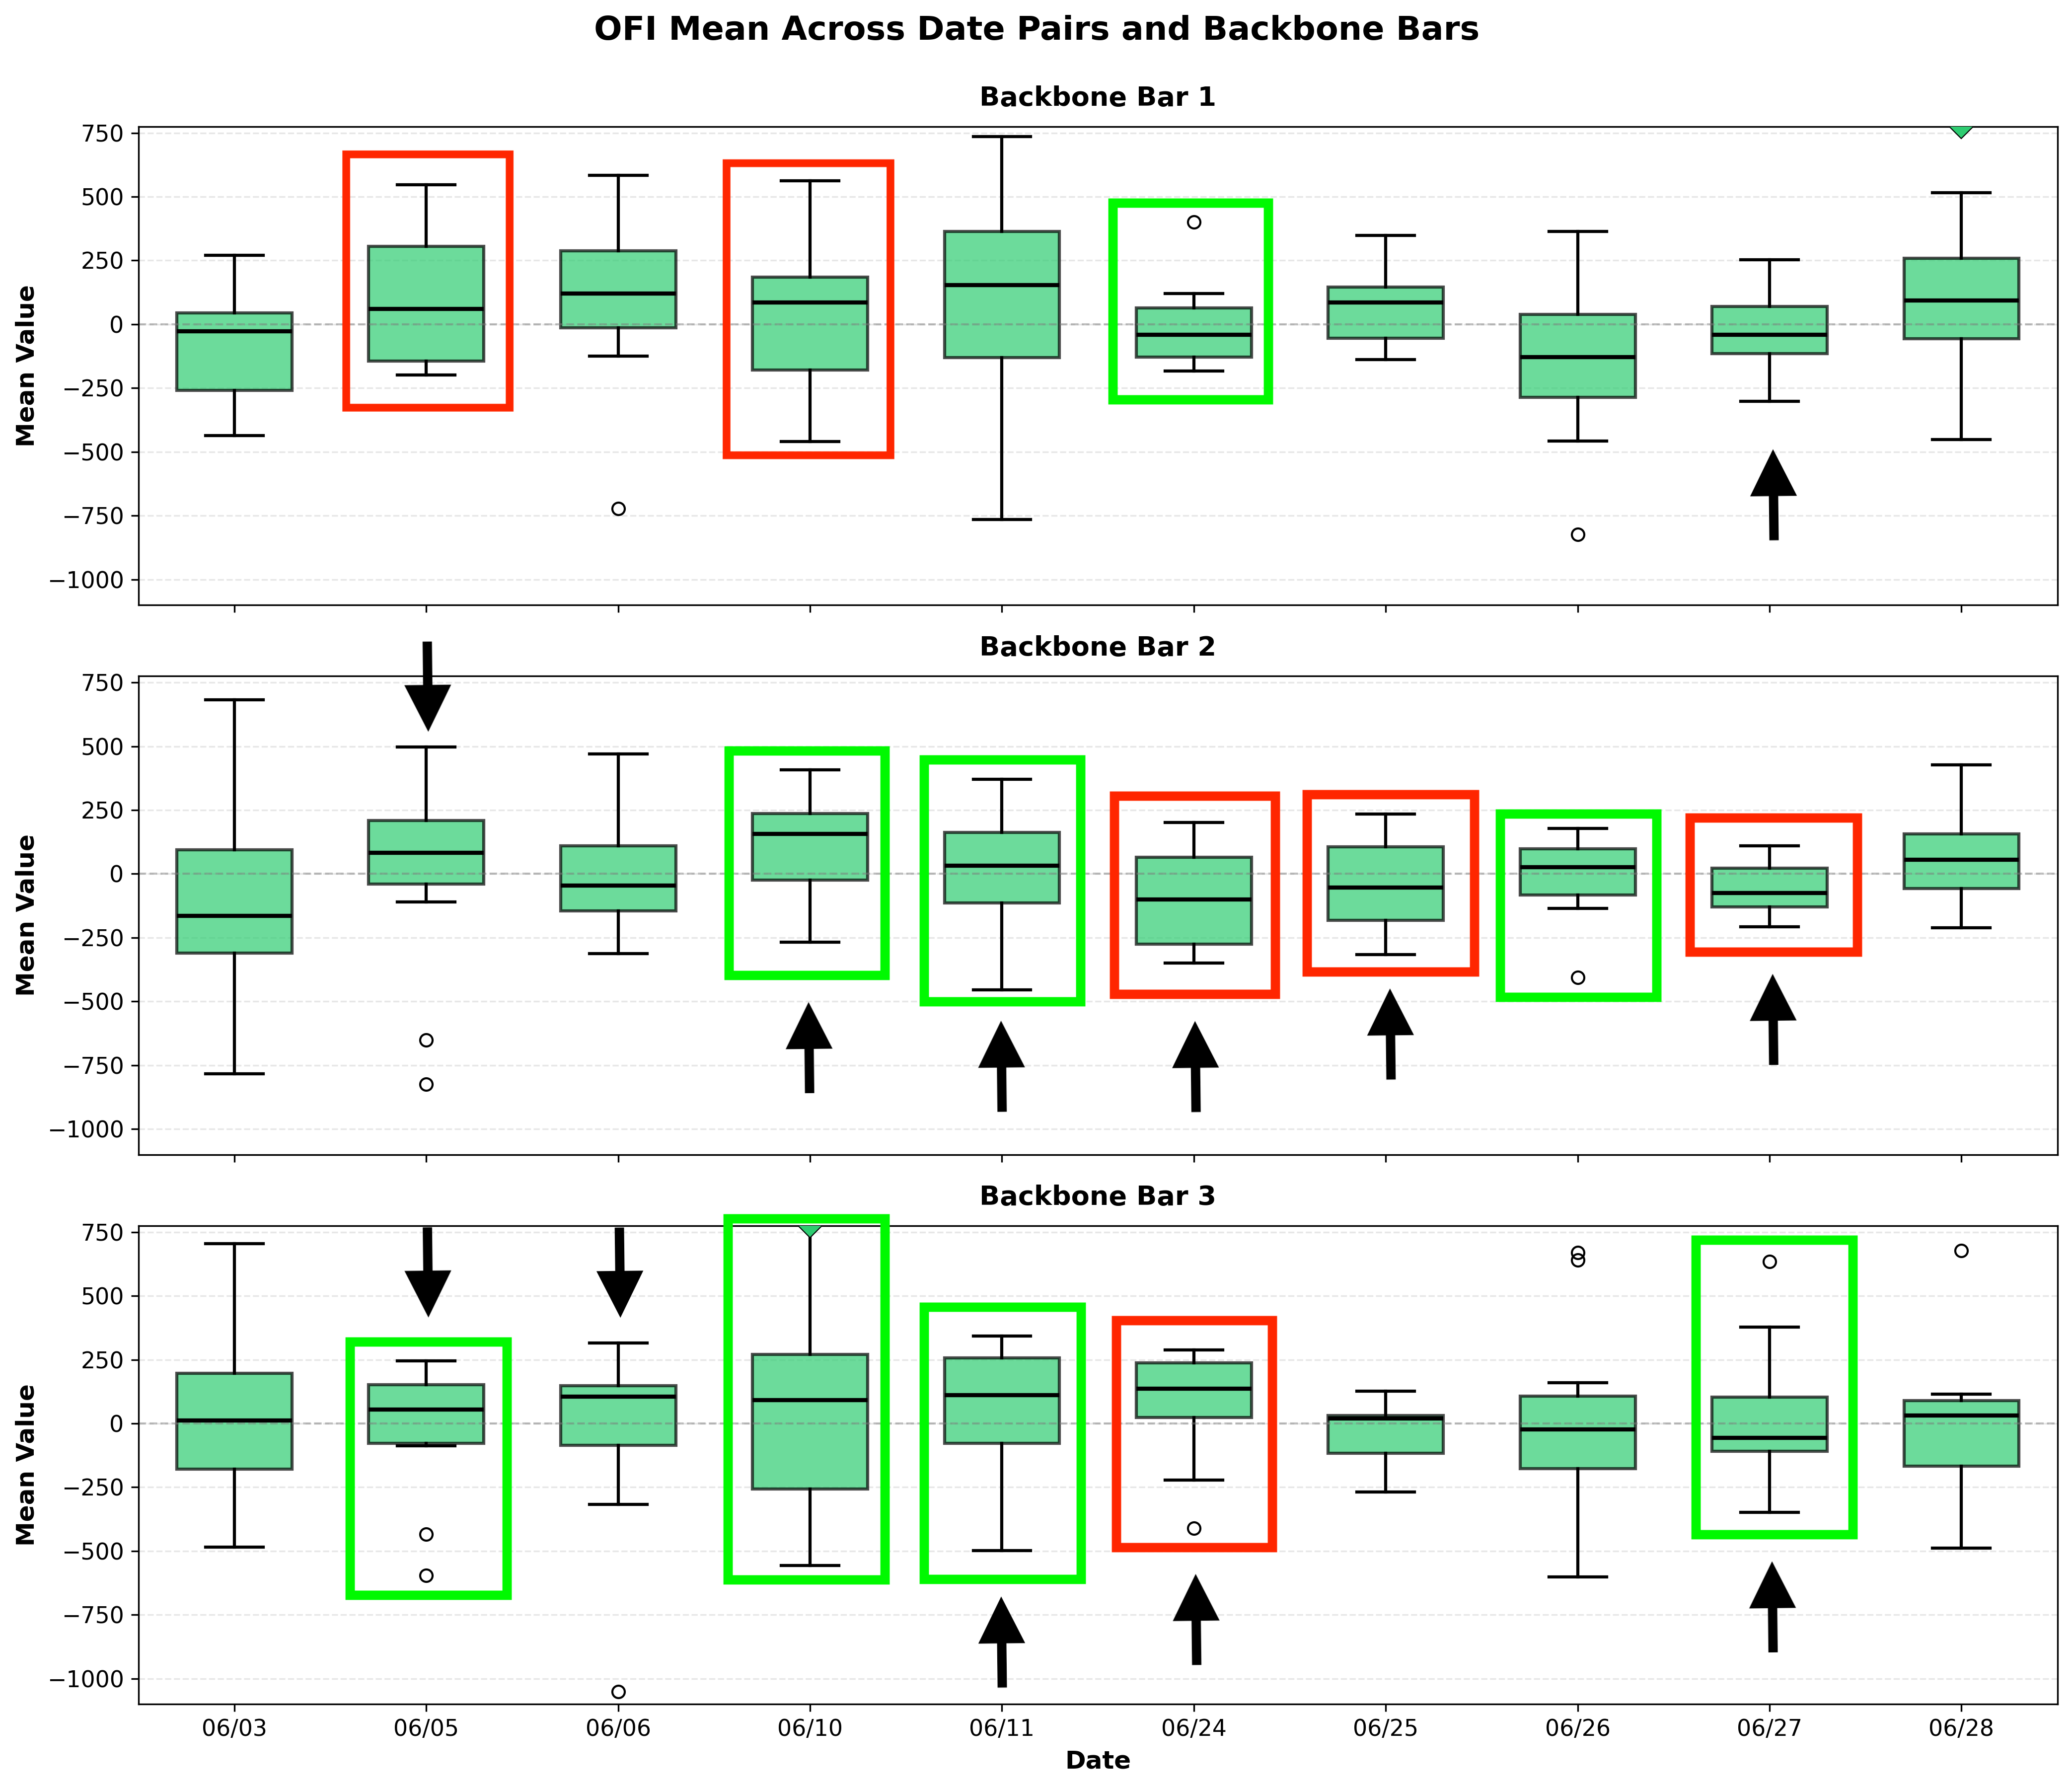
\includegraphics[width=0.9\linewidth]{ofi_aggregate_mean_boxplots_marked.png}
\caption{Distribution of the \textbf{mean} of the Order Flow Imbalance at touch ($OFI_{0, j}$) computed on each adapter bar and aggregated at the backbone bar level. See Figure~\ref{fig:sequential_boxplot_intc_data} for the interpretation of the markers.}
\label{fig:ofi_aggregate_mean}
\end{figure}

\begin{figure}[ht!]
\centering
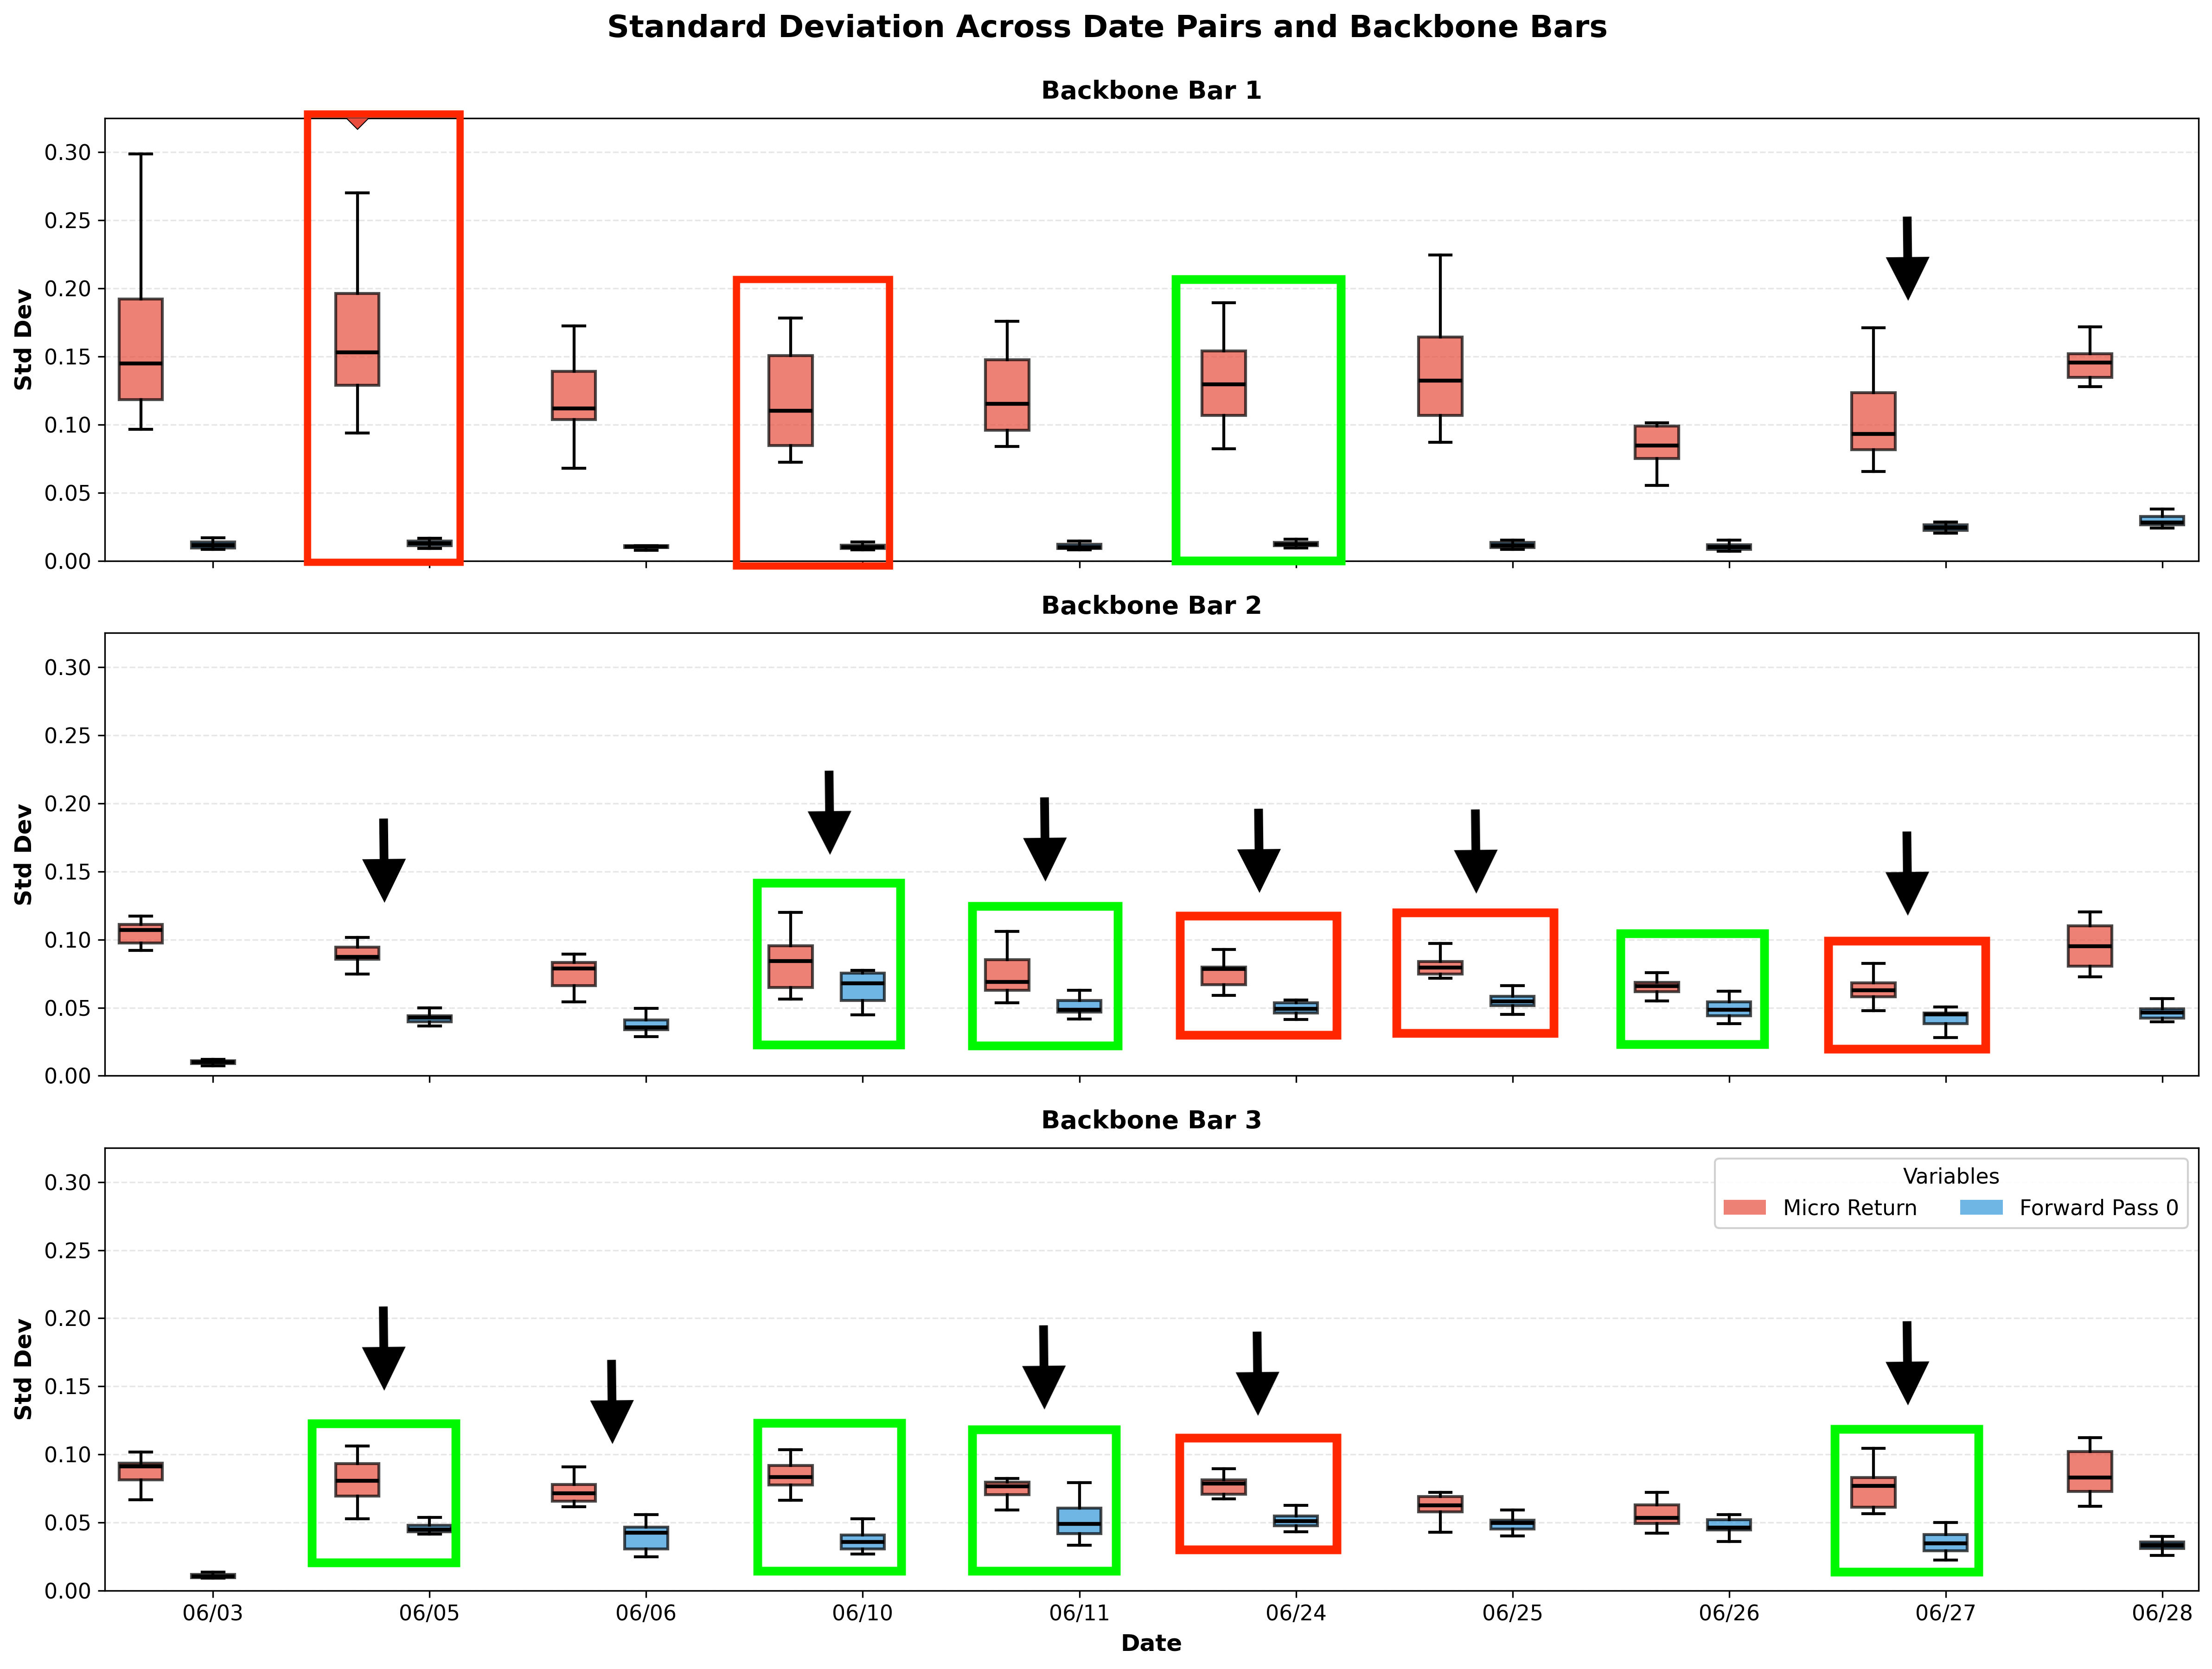
\includegraphics[width=0.9\linewidth]{covariate_aggregate_std_boxplots_marked.png}
\caption{Distribution of the \textbf{standard deviation} of the Micro-Return ($r^w_j$) and CNN-LSTM Output ($\mathrm{CNNLSTM}_{\mathbf{W}}\!\left(\widetilde{\mathbf{OF}}^{\mathcal{P}^{(E)}}_{i_{t-1}-99:i_{t-1}}\right)$) computed on each adapter bar and aggregated at the backbone bar level. See Figure~\ref{fig:sequential_boxplot_intc_data} for the interpretation of the markers.}
\label{fig:covariate_aggregate_std}
\end{figure}

\begin{figure}[ht!]
\centering
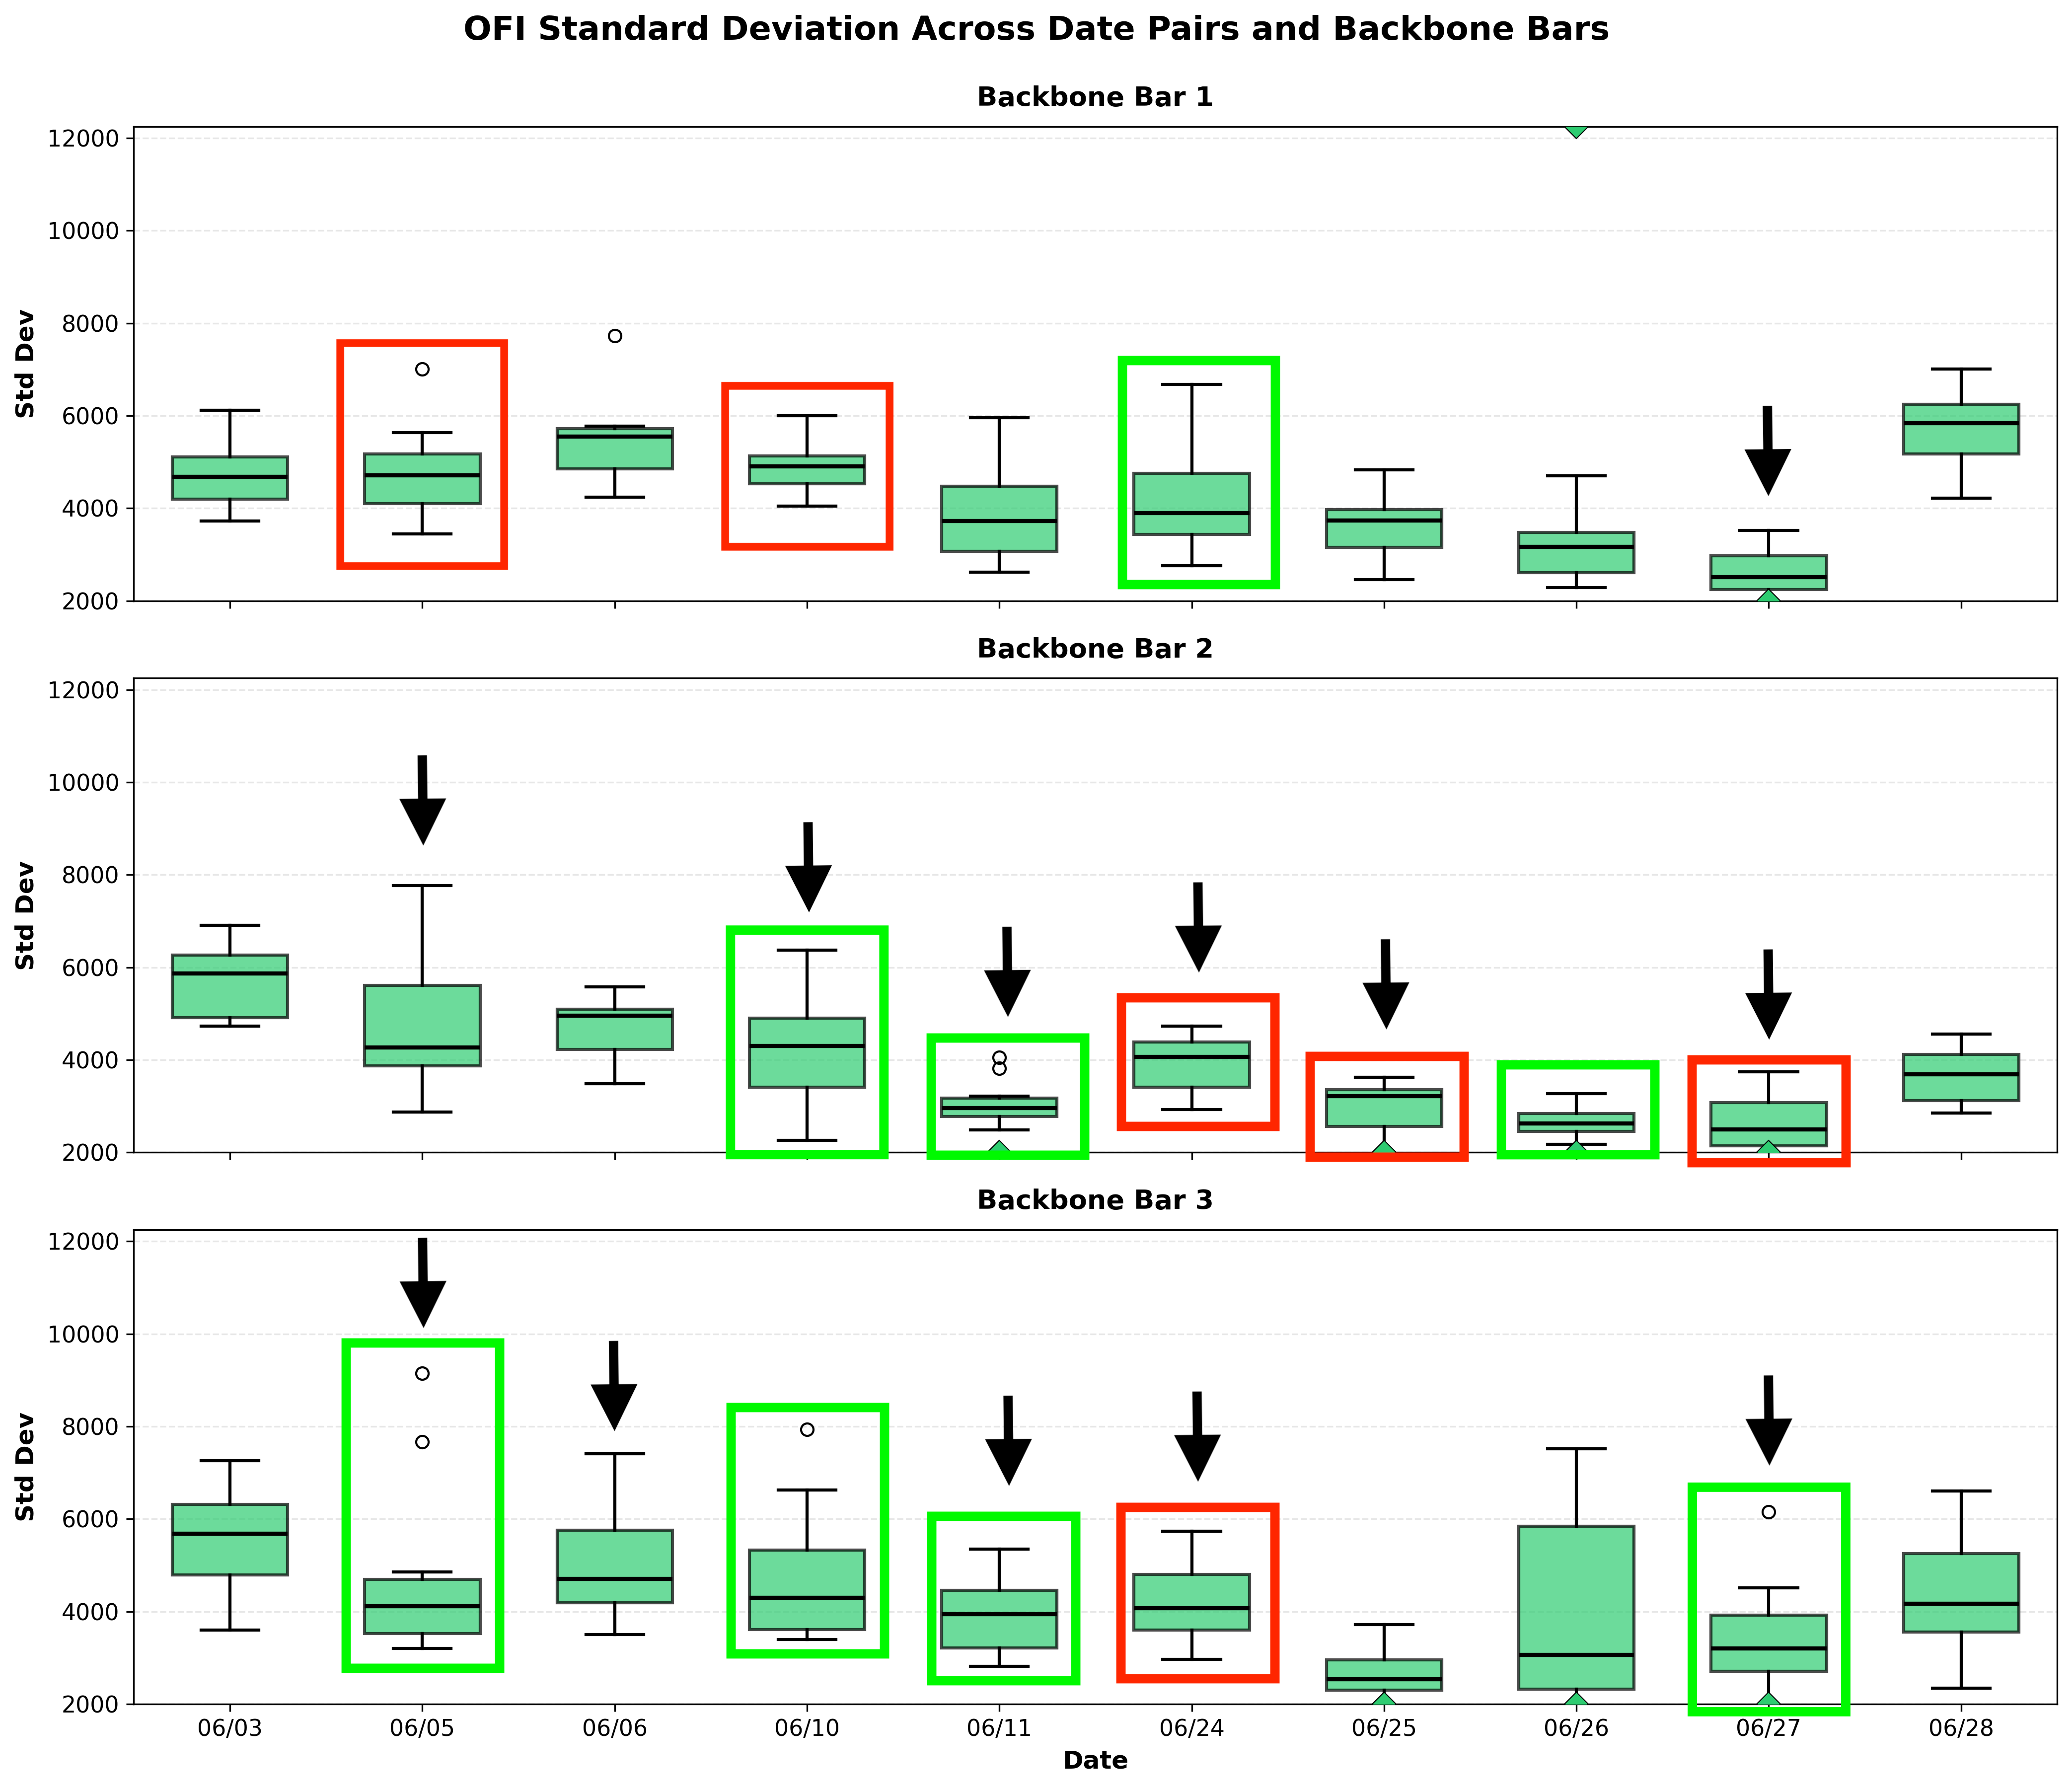
\includegraphics[width=0.9\linewidth]{ofi_aggregate_std_boxplots_marked.png}
\caption{Distribution of the \textbf{standard deviation} of the Order Flow Imbalance at touch ($OFI_{0, j}$) computed on each adapter bar and aggregated at the backbone bar level. See Figure~\ref{fig:sequential_boxplot_intc_data} for the interpretation of the markers.}
\label{fig:ofi_aggregate_std}
\end{figure}


\begin{figure}[ht!]
\centering
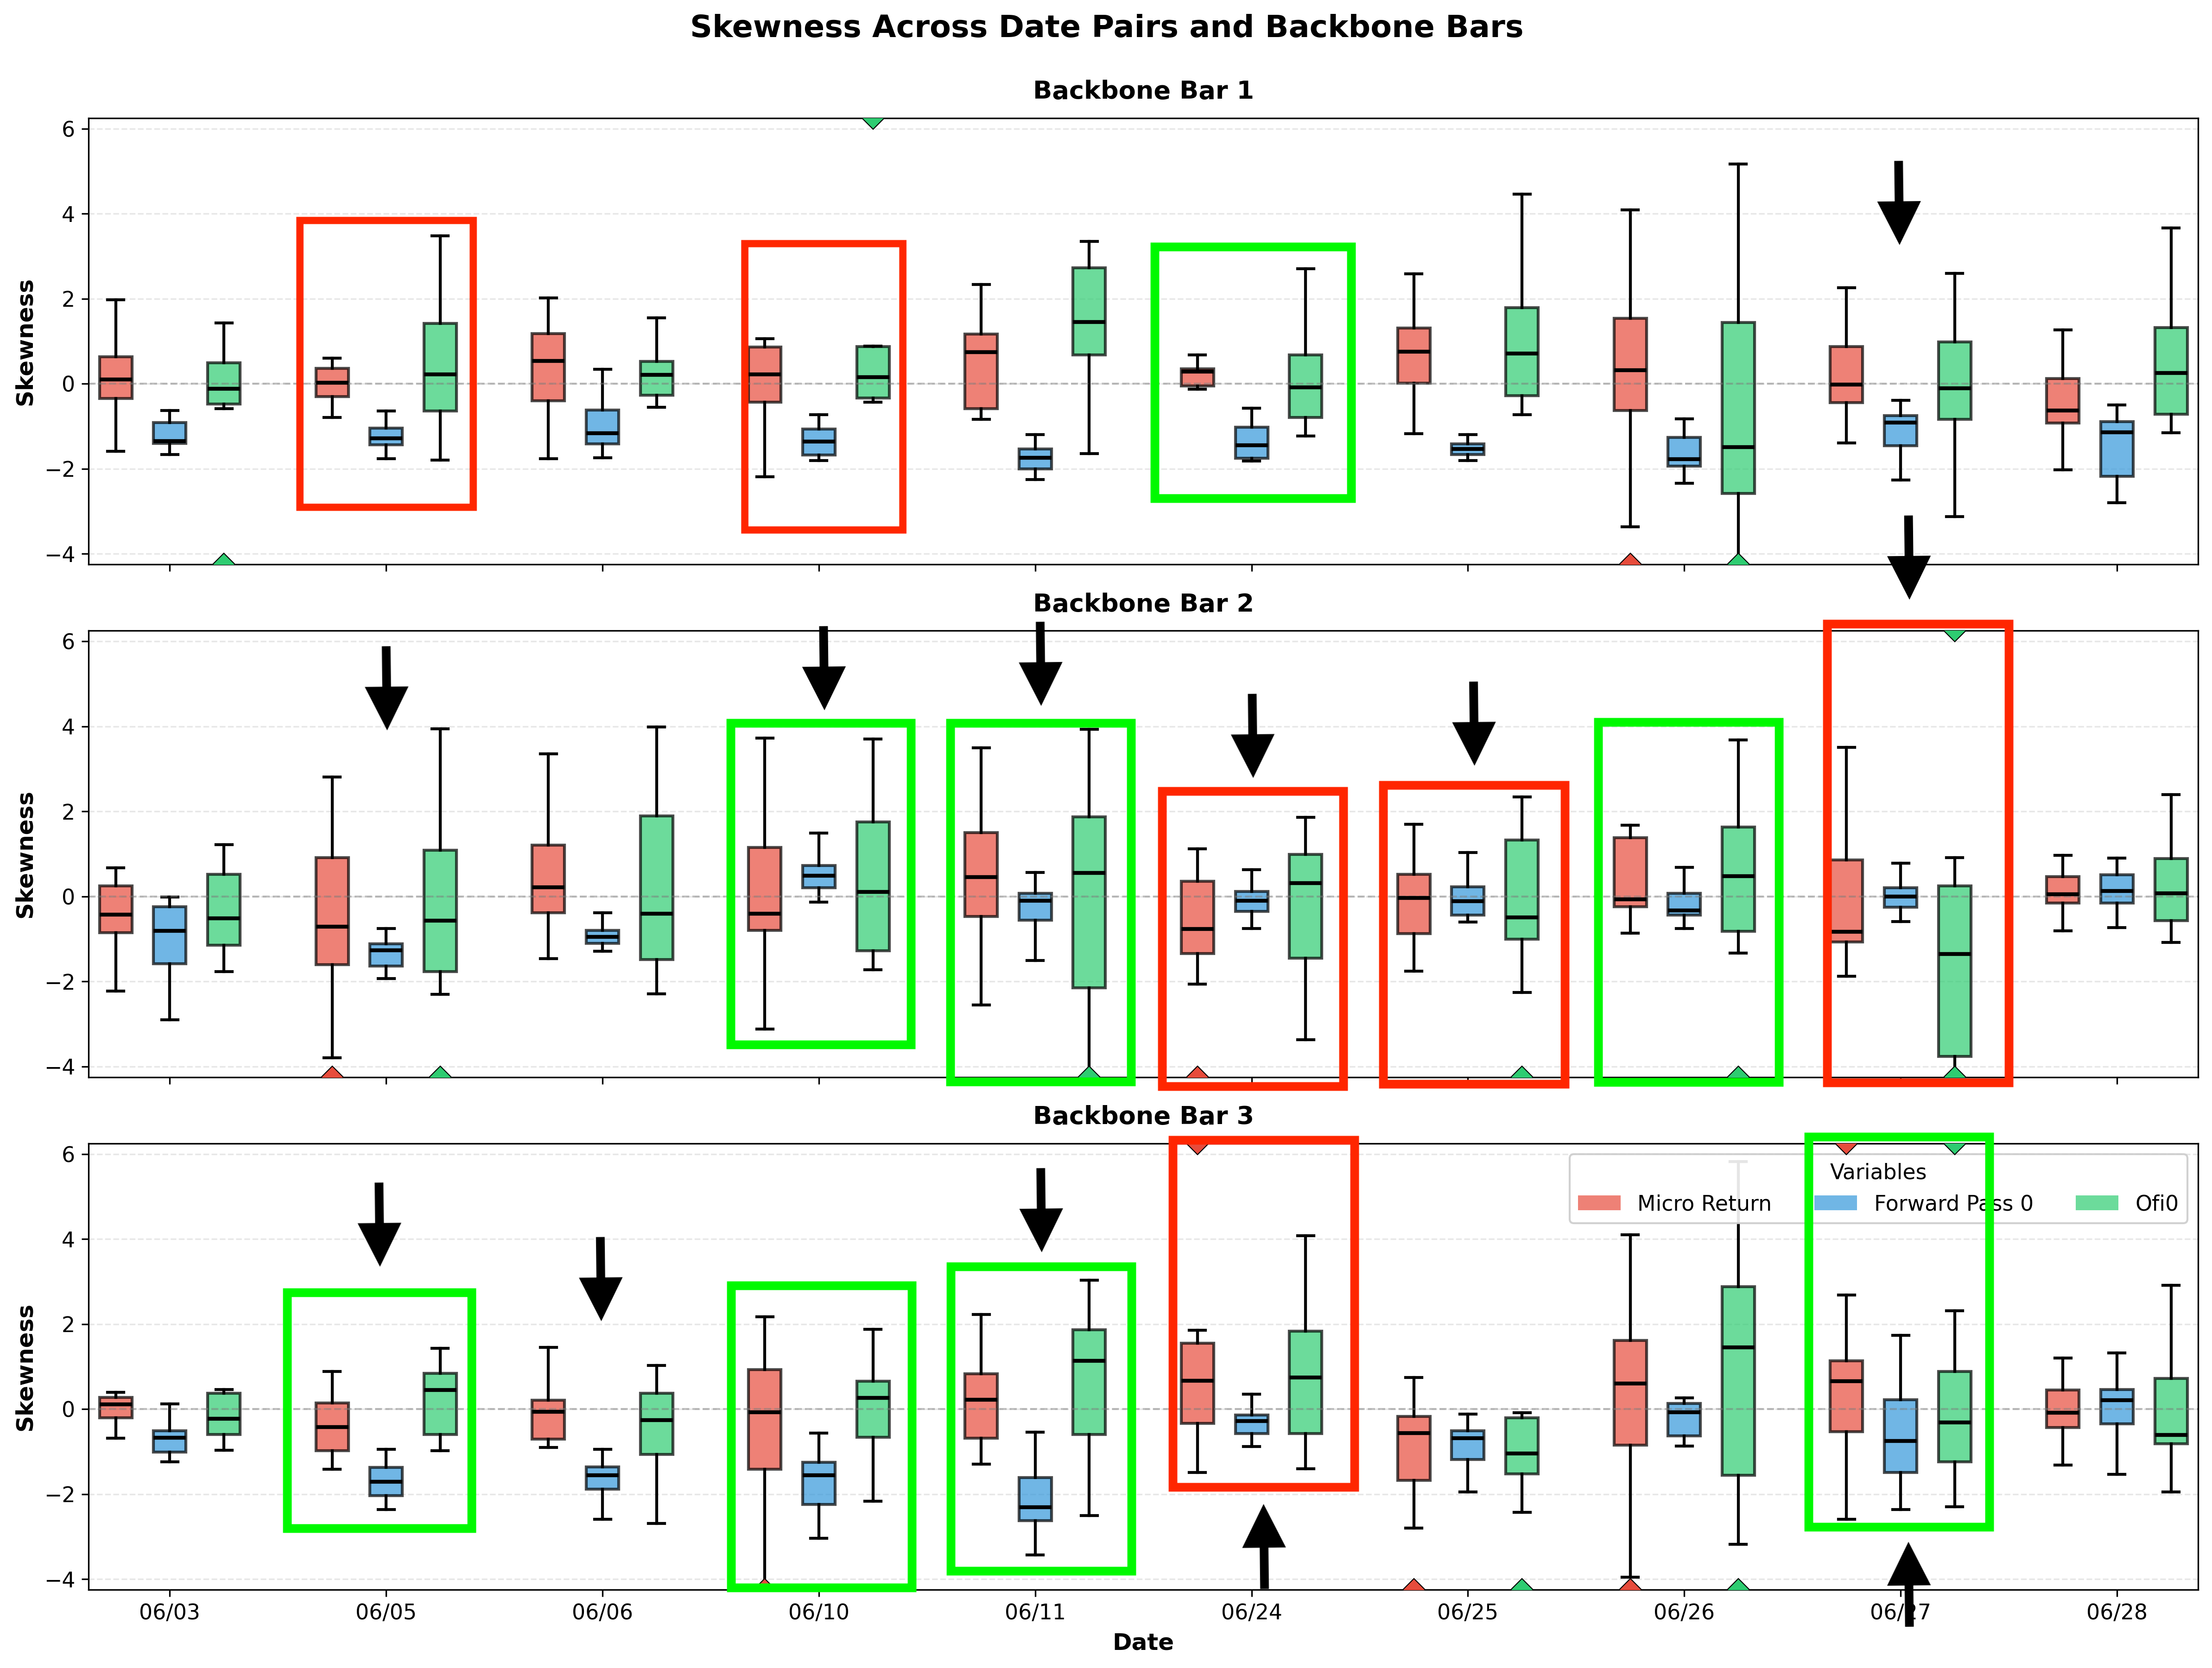
\includegraphics[width=0.9\linewidth]{covariate_aggregate_skewness_boxplots_marked.png}
\caption{Distribution of the \textbf{skewness} of the Micro-Return ($r^w_j$), CNN-LSTM Output ($\mathrm{CNNLSTM}_{\mathbf{W}}\!\left(\widetilde{\mathbf{OF}}^{\mathcal{P}^{(E)}}_{i_{t-1}-99:i_{t-1}}\right)$), and Order Flow Imbalance at touch ($OFI_{0, j}$) computed on each adapter bar and aggregated at the backbone bar level. See Figure~\ref{fig:sequential_boxplot_intc_data} for the interpretation of the markers.}
\label{fig:covariate_aggregate_skewness}
\end{figure}

\begin{figure}[ht!]
\centering
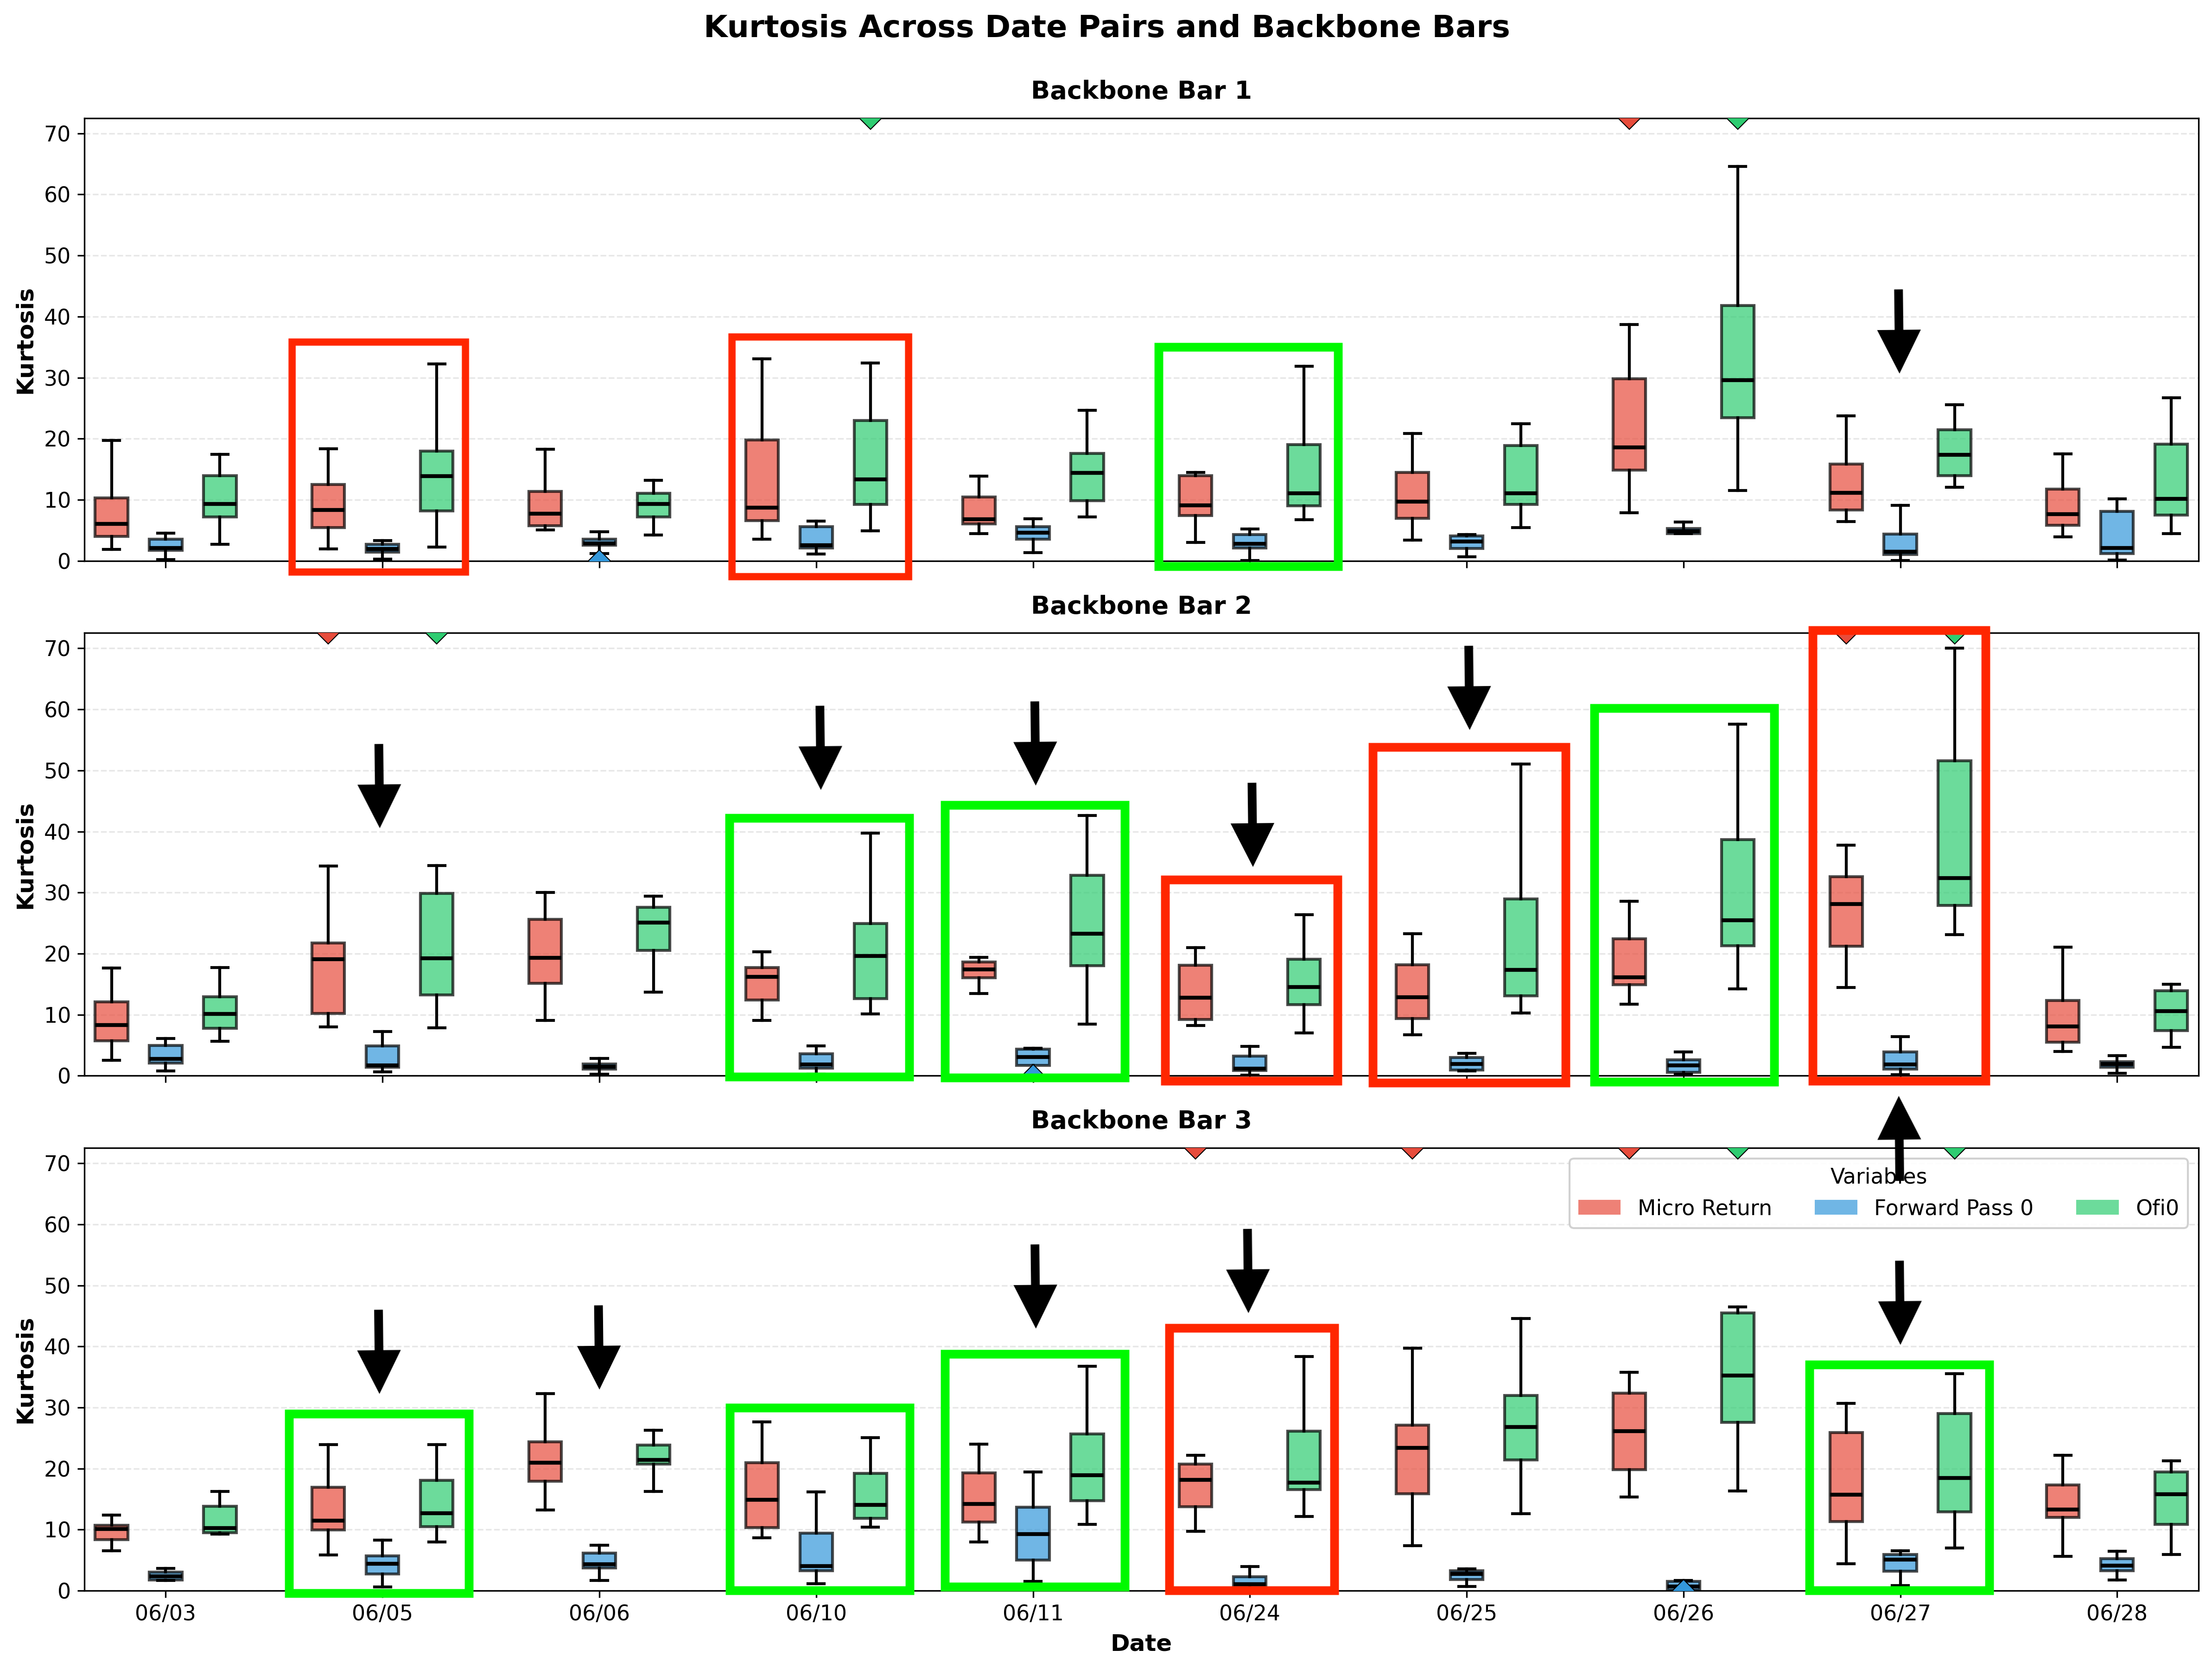
\includegraphics[width=0.9\linewidth]{covariate_aggregate_kurtosis_boxplots_marked.png}
\caption{Distribution of the \textbf{kurtosis} of the Micro-Return ($r^w_j$), CNN-LSTM Output ($\mathrm{CNNLSTM}_{\mathbf{W}}\!\left(\widetilde{\mathbf{OF}}^{\mathcal{P}^{(E)}}_{i_{t-1}-99:i_{t-1}}\right)$), and Order Flow Imbalance at touch ($OFI_{0, j}$) computed on each adapter bar and aggregated at the backbone bar level. See Figure~\ref{fig:sequential_boxplot_intc_data} for the interpretation of the markers.}
\label{fig:covariate_aggregate_kurtosis}
\end{figure}

\begin{figure}[ht!]
\centering
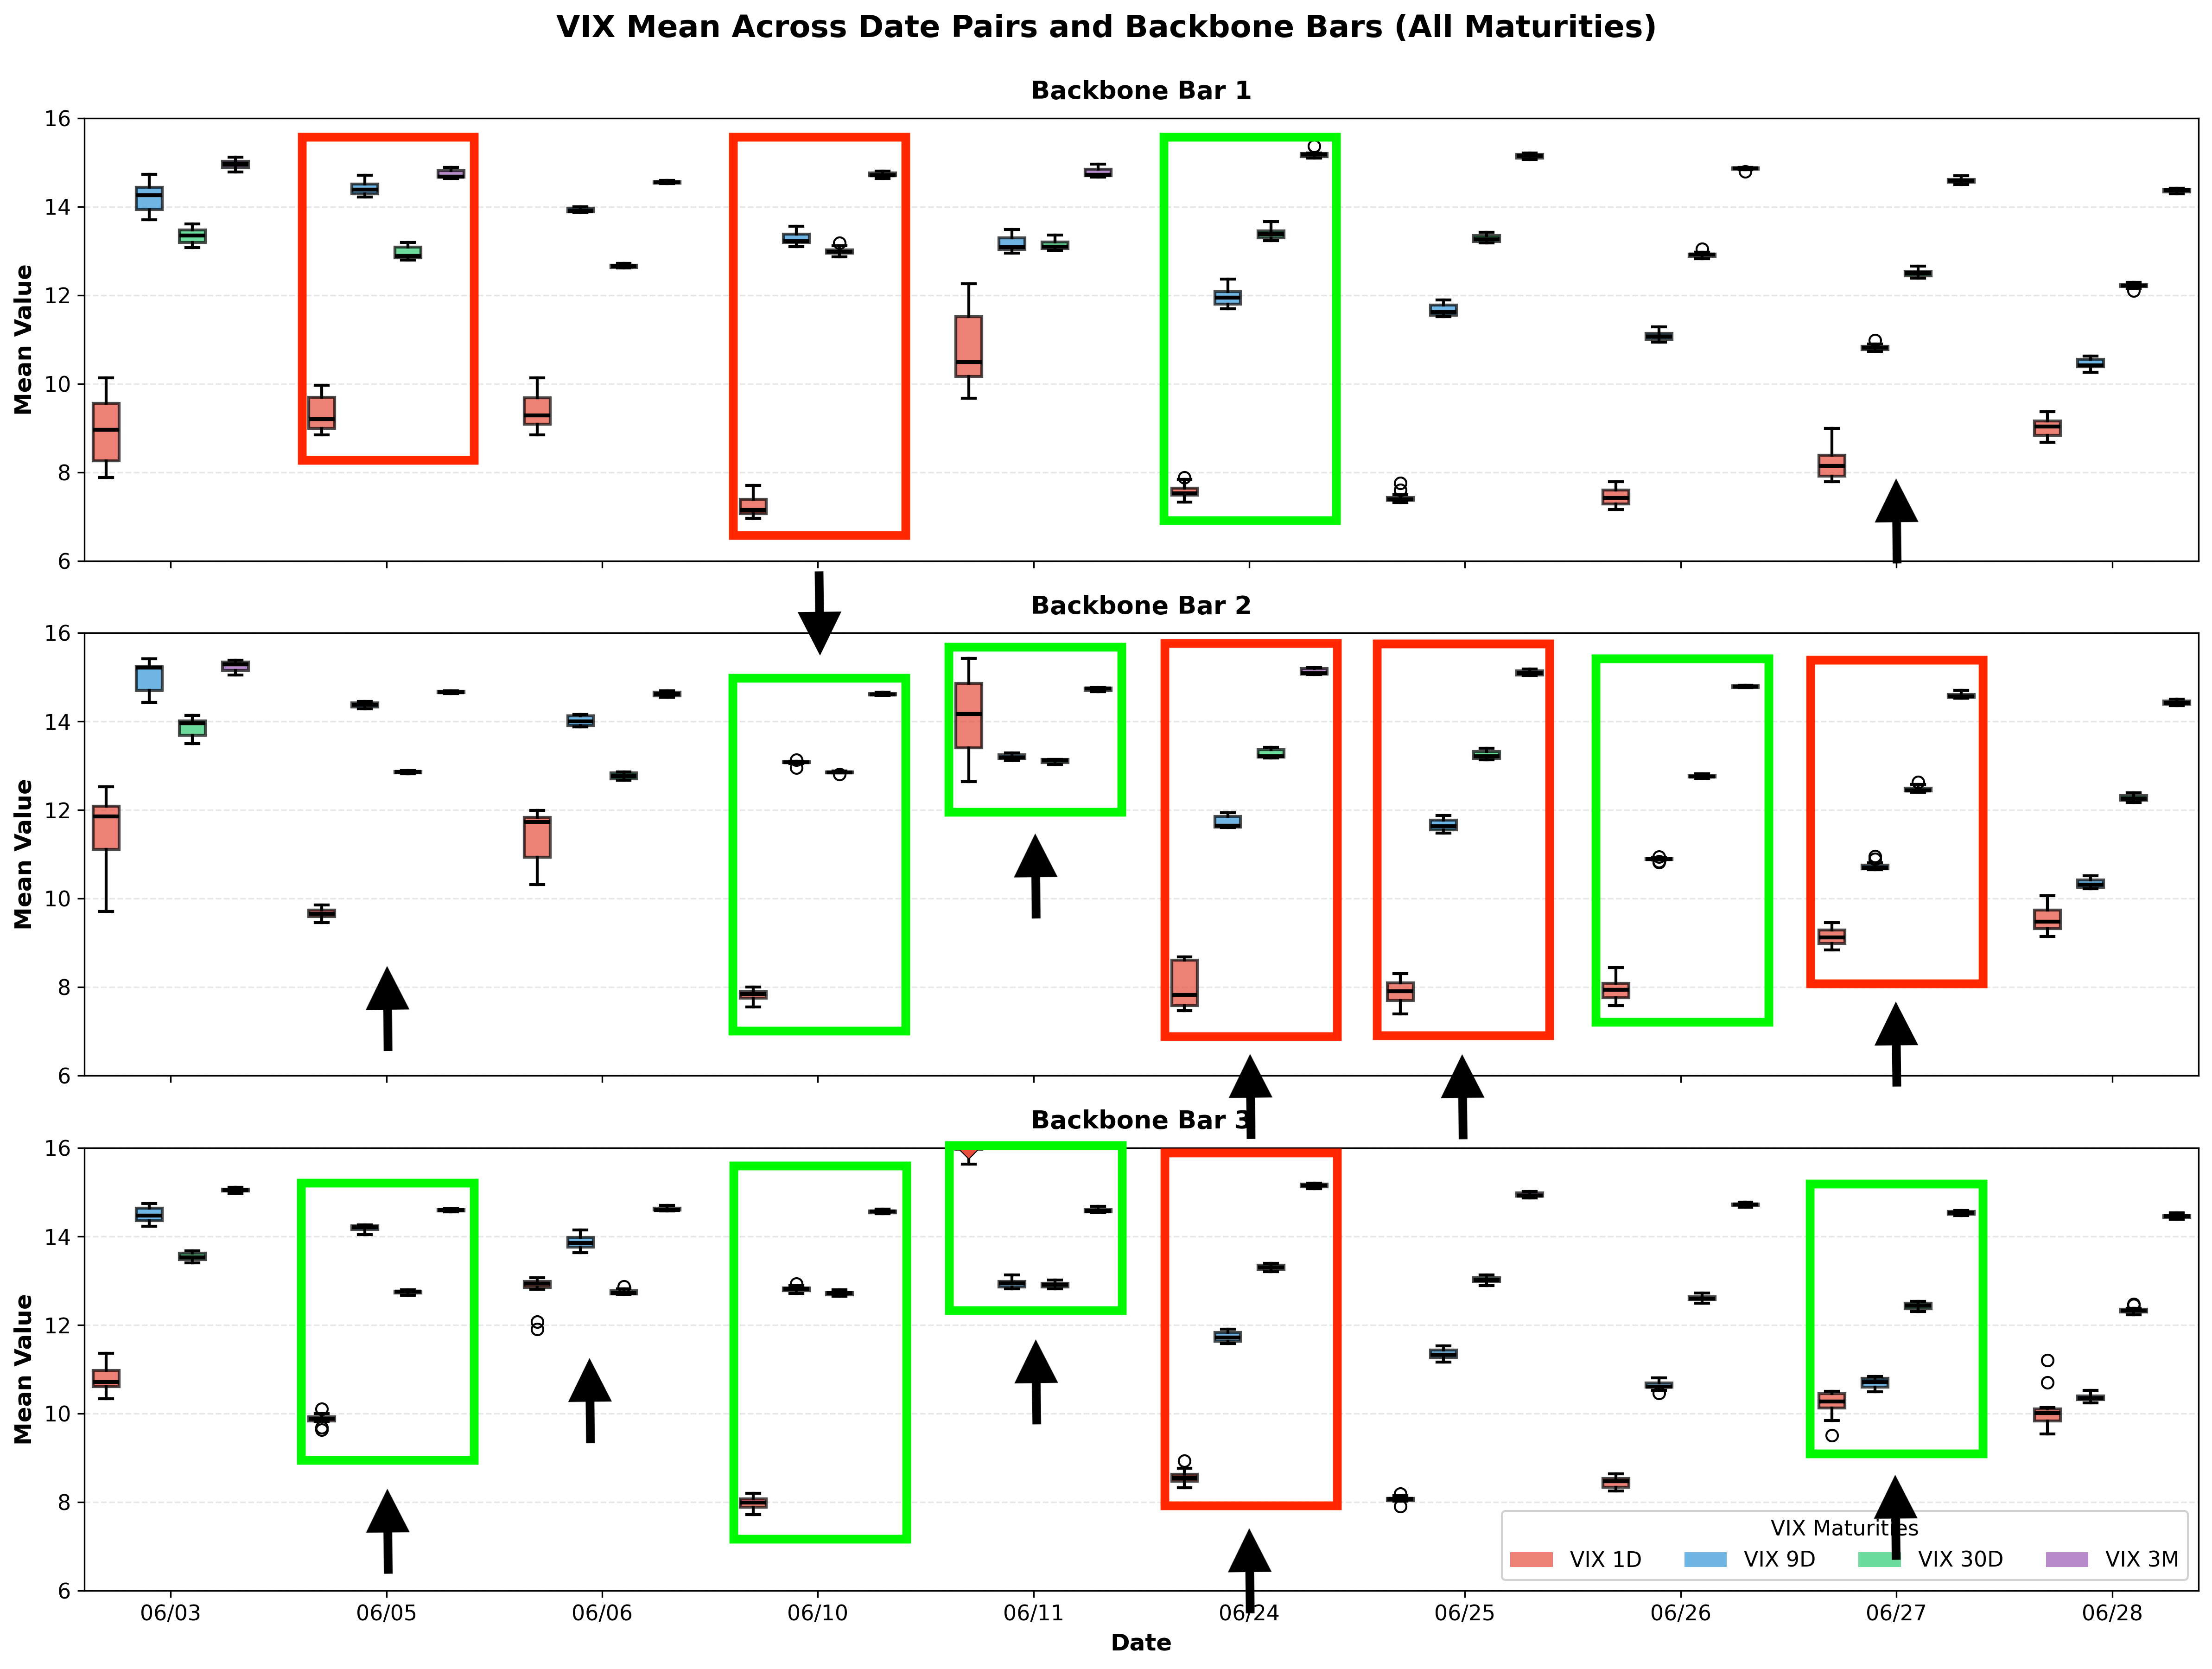
\includegraphics[width=0.9\linewidth]{vix_aggregate_mean_boxplots_marked.png}
\caption{Distribution of the \textbf{mean} of the VIX indices ($VIX_t^{(\tau)}$ for $\tau \in \{ \text{1d}, \text{9d}, \text{30d}, \text{3m} \}$) computed on each adapter bar and aggregated at the backbone bar level. See Figure~\ref{fig:sequential_boxplot_intc_data} for the interpretation of the markers.}
\label{fig:vix_aggregate_mean}
\end{figure}

\begin{figure}[ht!]
\centering
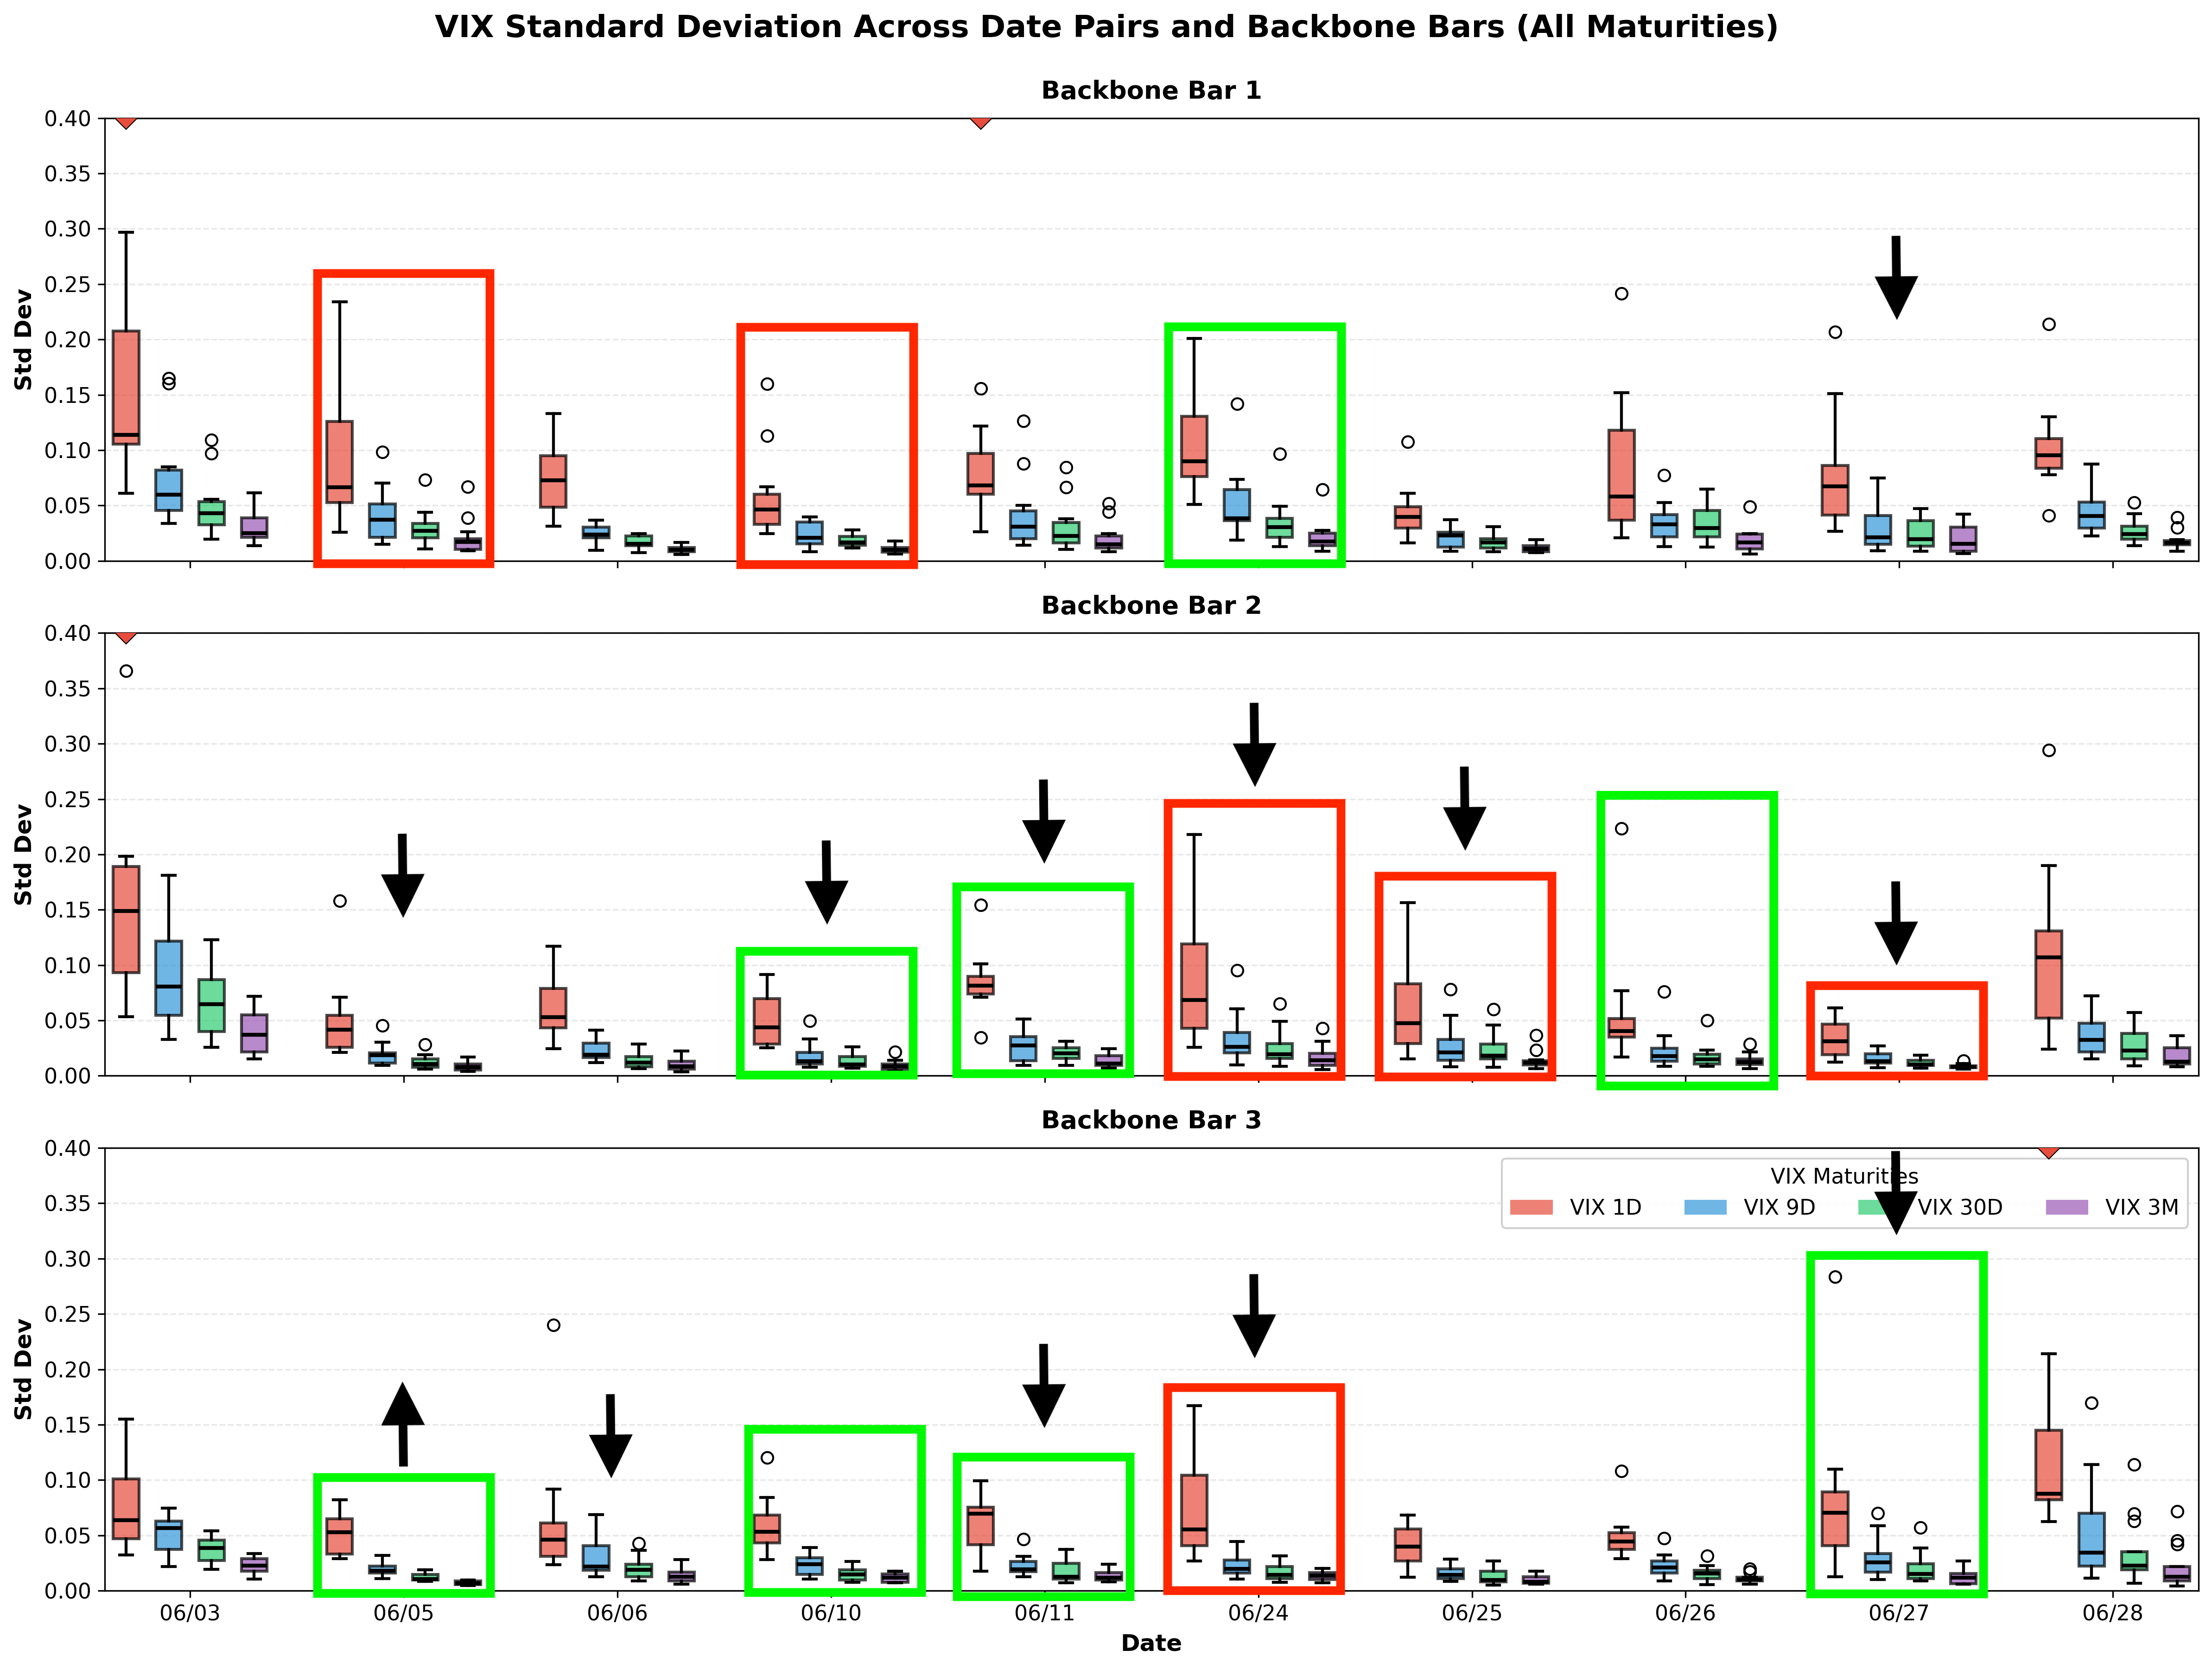
\includegraphics[width=0.9\linewidth]{vix_aggregate_std_boxplots_marked.png}
\caption{Distribution of the \textbf{standard deviation} of the VIX indices ($VIX_t^{(\tau)}$ for $\tau \in \{ \text{1d}, \text{9d}, \text{30d}, \text{3m} \}$) computed on each adapter bar and aggregated at the backbone bar level. See Figure~\ref{fig:sequential_boxplot_intc_data} for the interpretation of the markers.}
\label{fig:vix_aggregate_std}
\end{figure}

\begin{figure}[ht!]
\centering
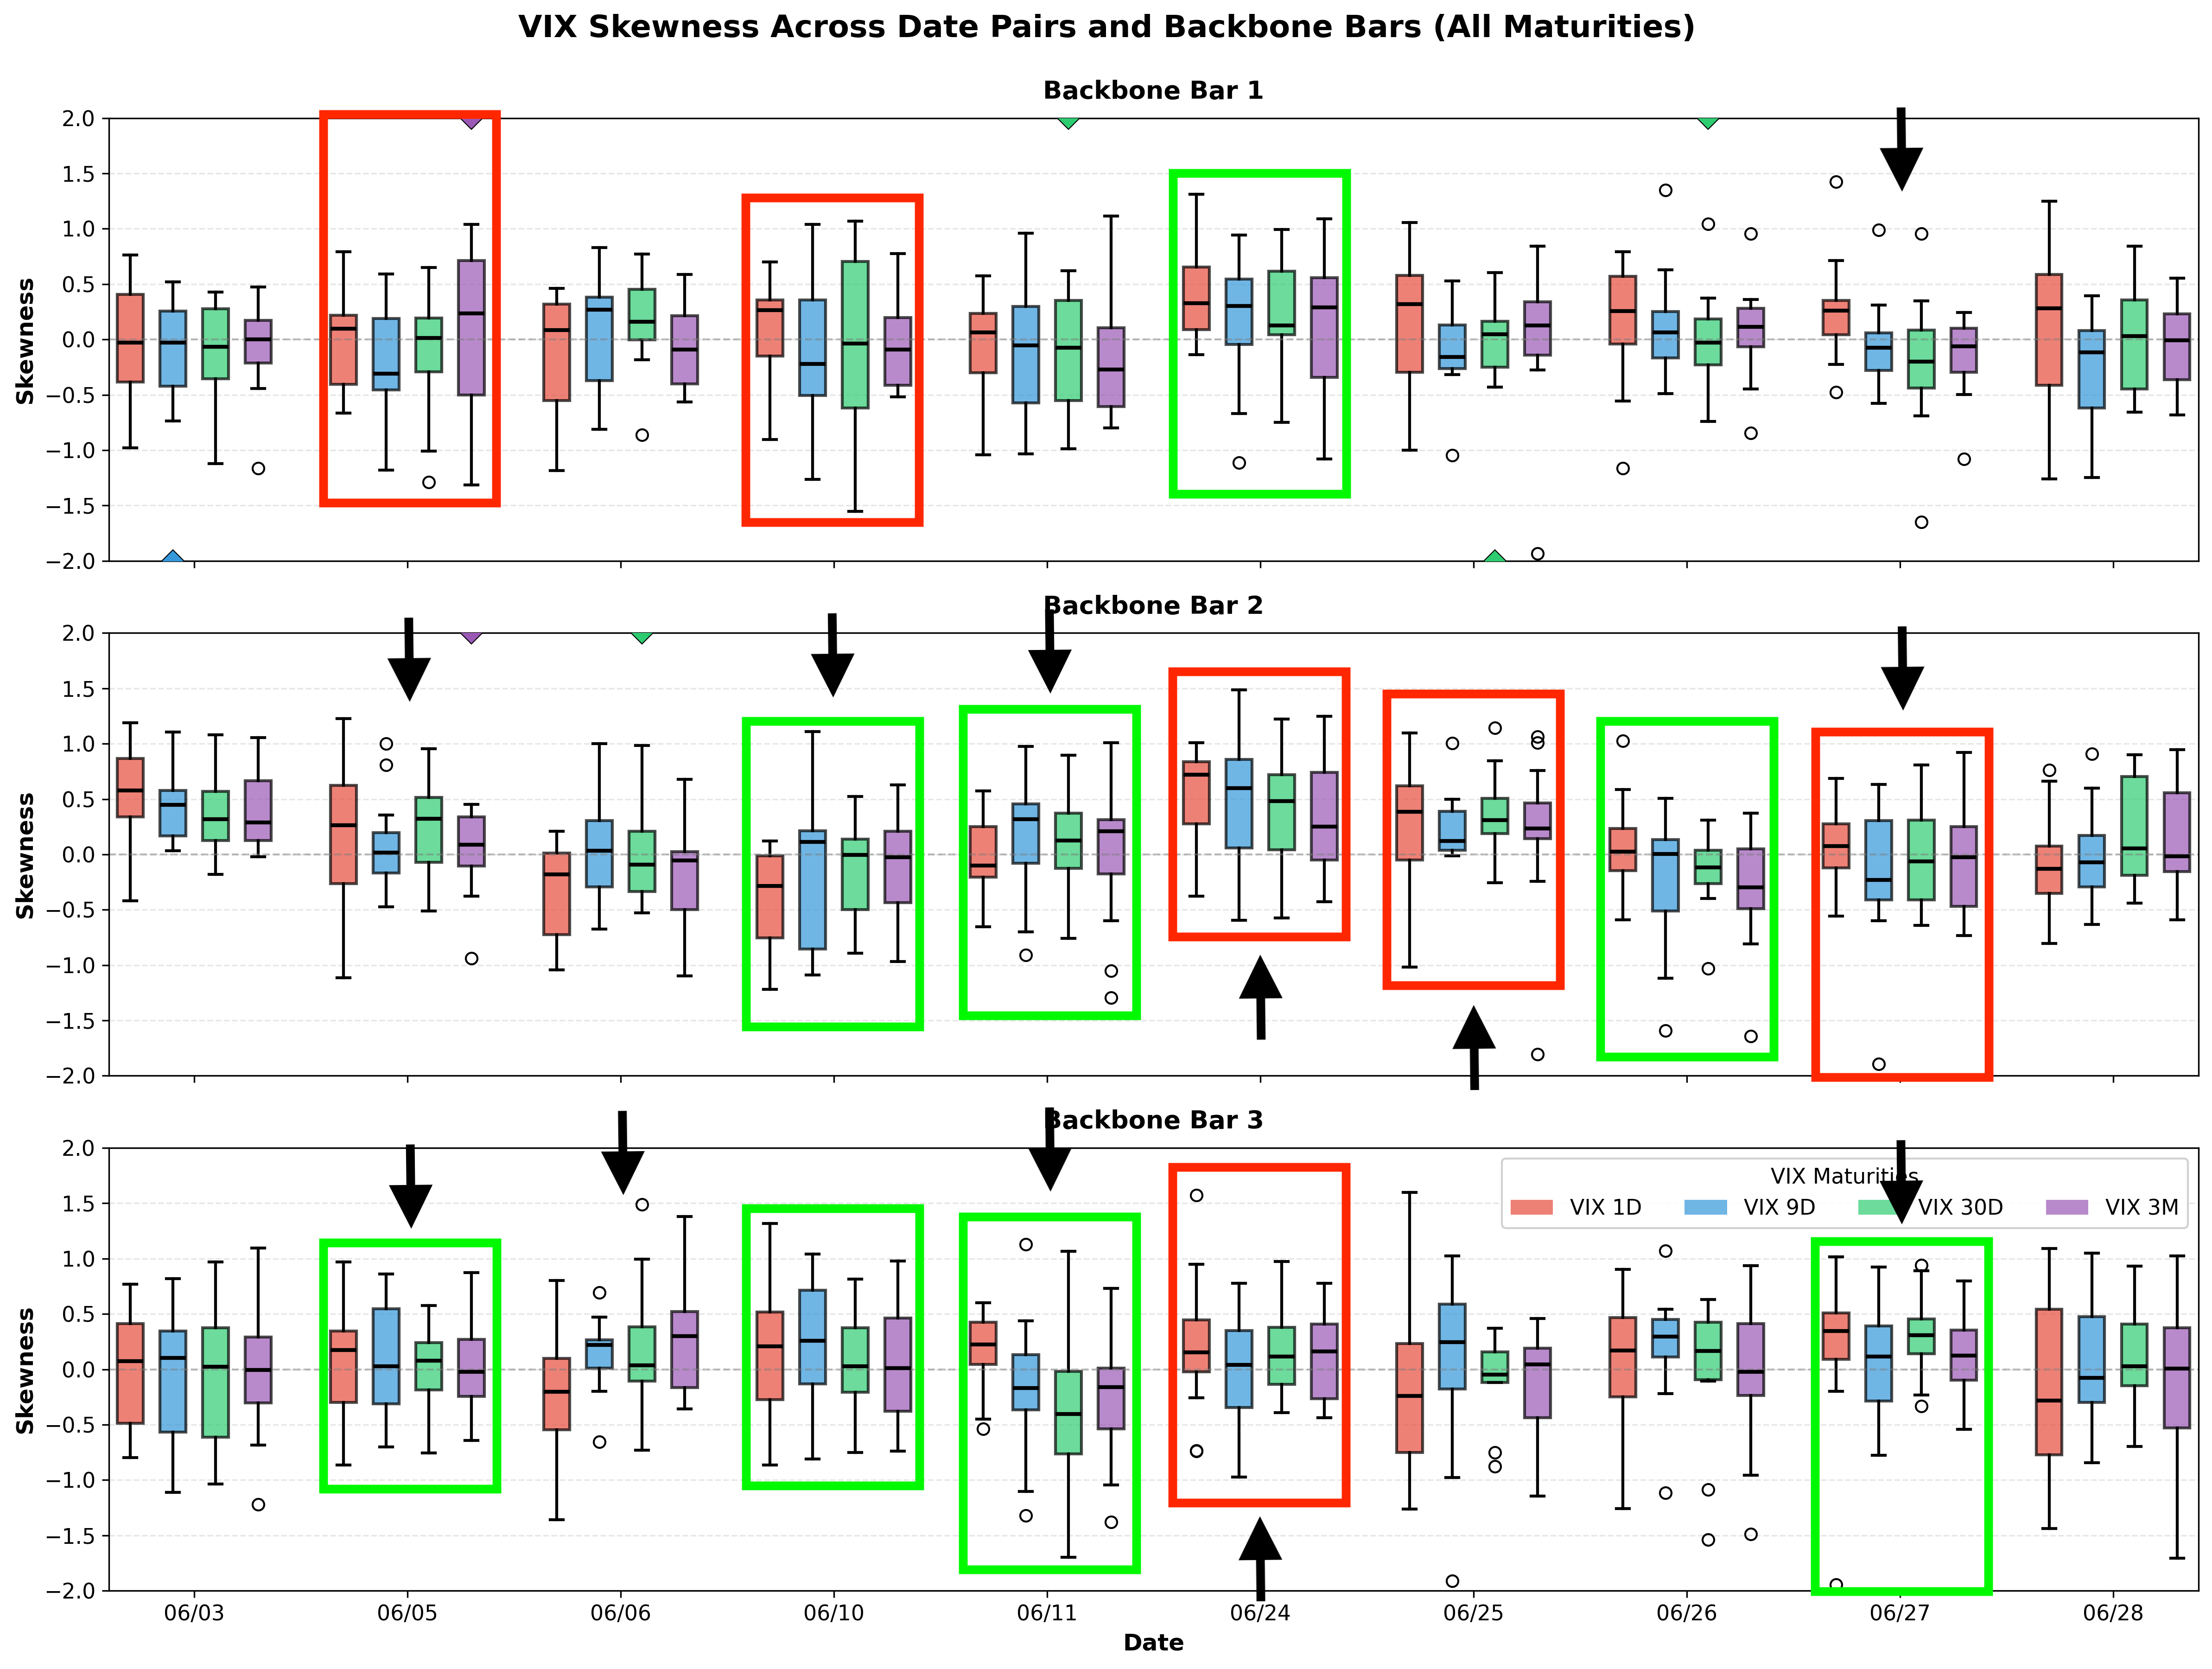
\includegraphics[width=0.9\linewidth]{vix_aggregate_skewness_boxplots_marked.png}
\caption{Distribution of the \textbf{skewness} of the VIX indices ($VIX_t^{(\tau)}$ for $\tau \in \{ \text{1d}, \text{9d}, \text{30d}, \text{3m} \}$) computed on each adapter bar and aggregated at the backbone bar level. See Figure~\ref{fig:sequential_boxplot_intc_data} for the interpretation of the markers.}
\label{fig:vix_aggregate_skewness}
\end{figure}

\begin{figure}[ht!]
\centering
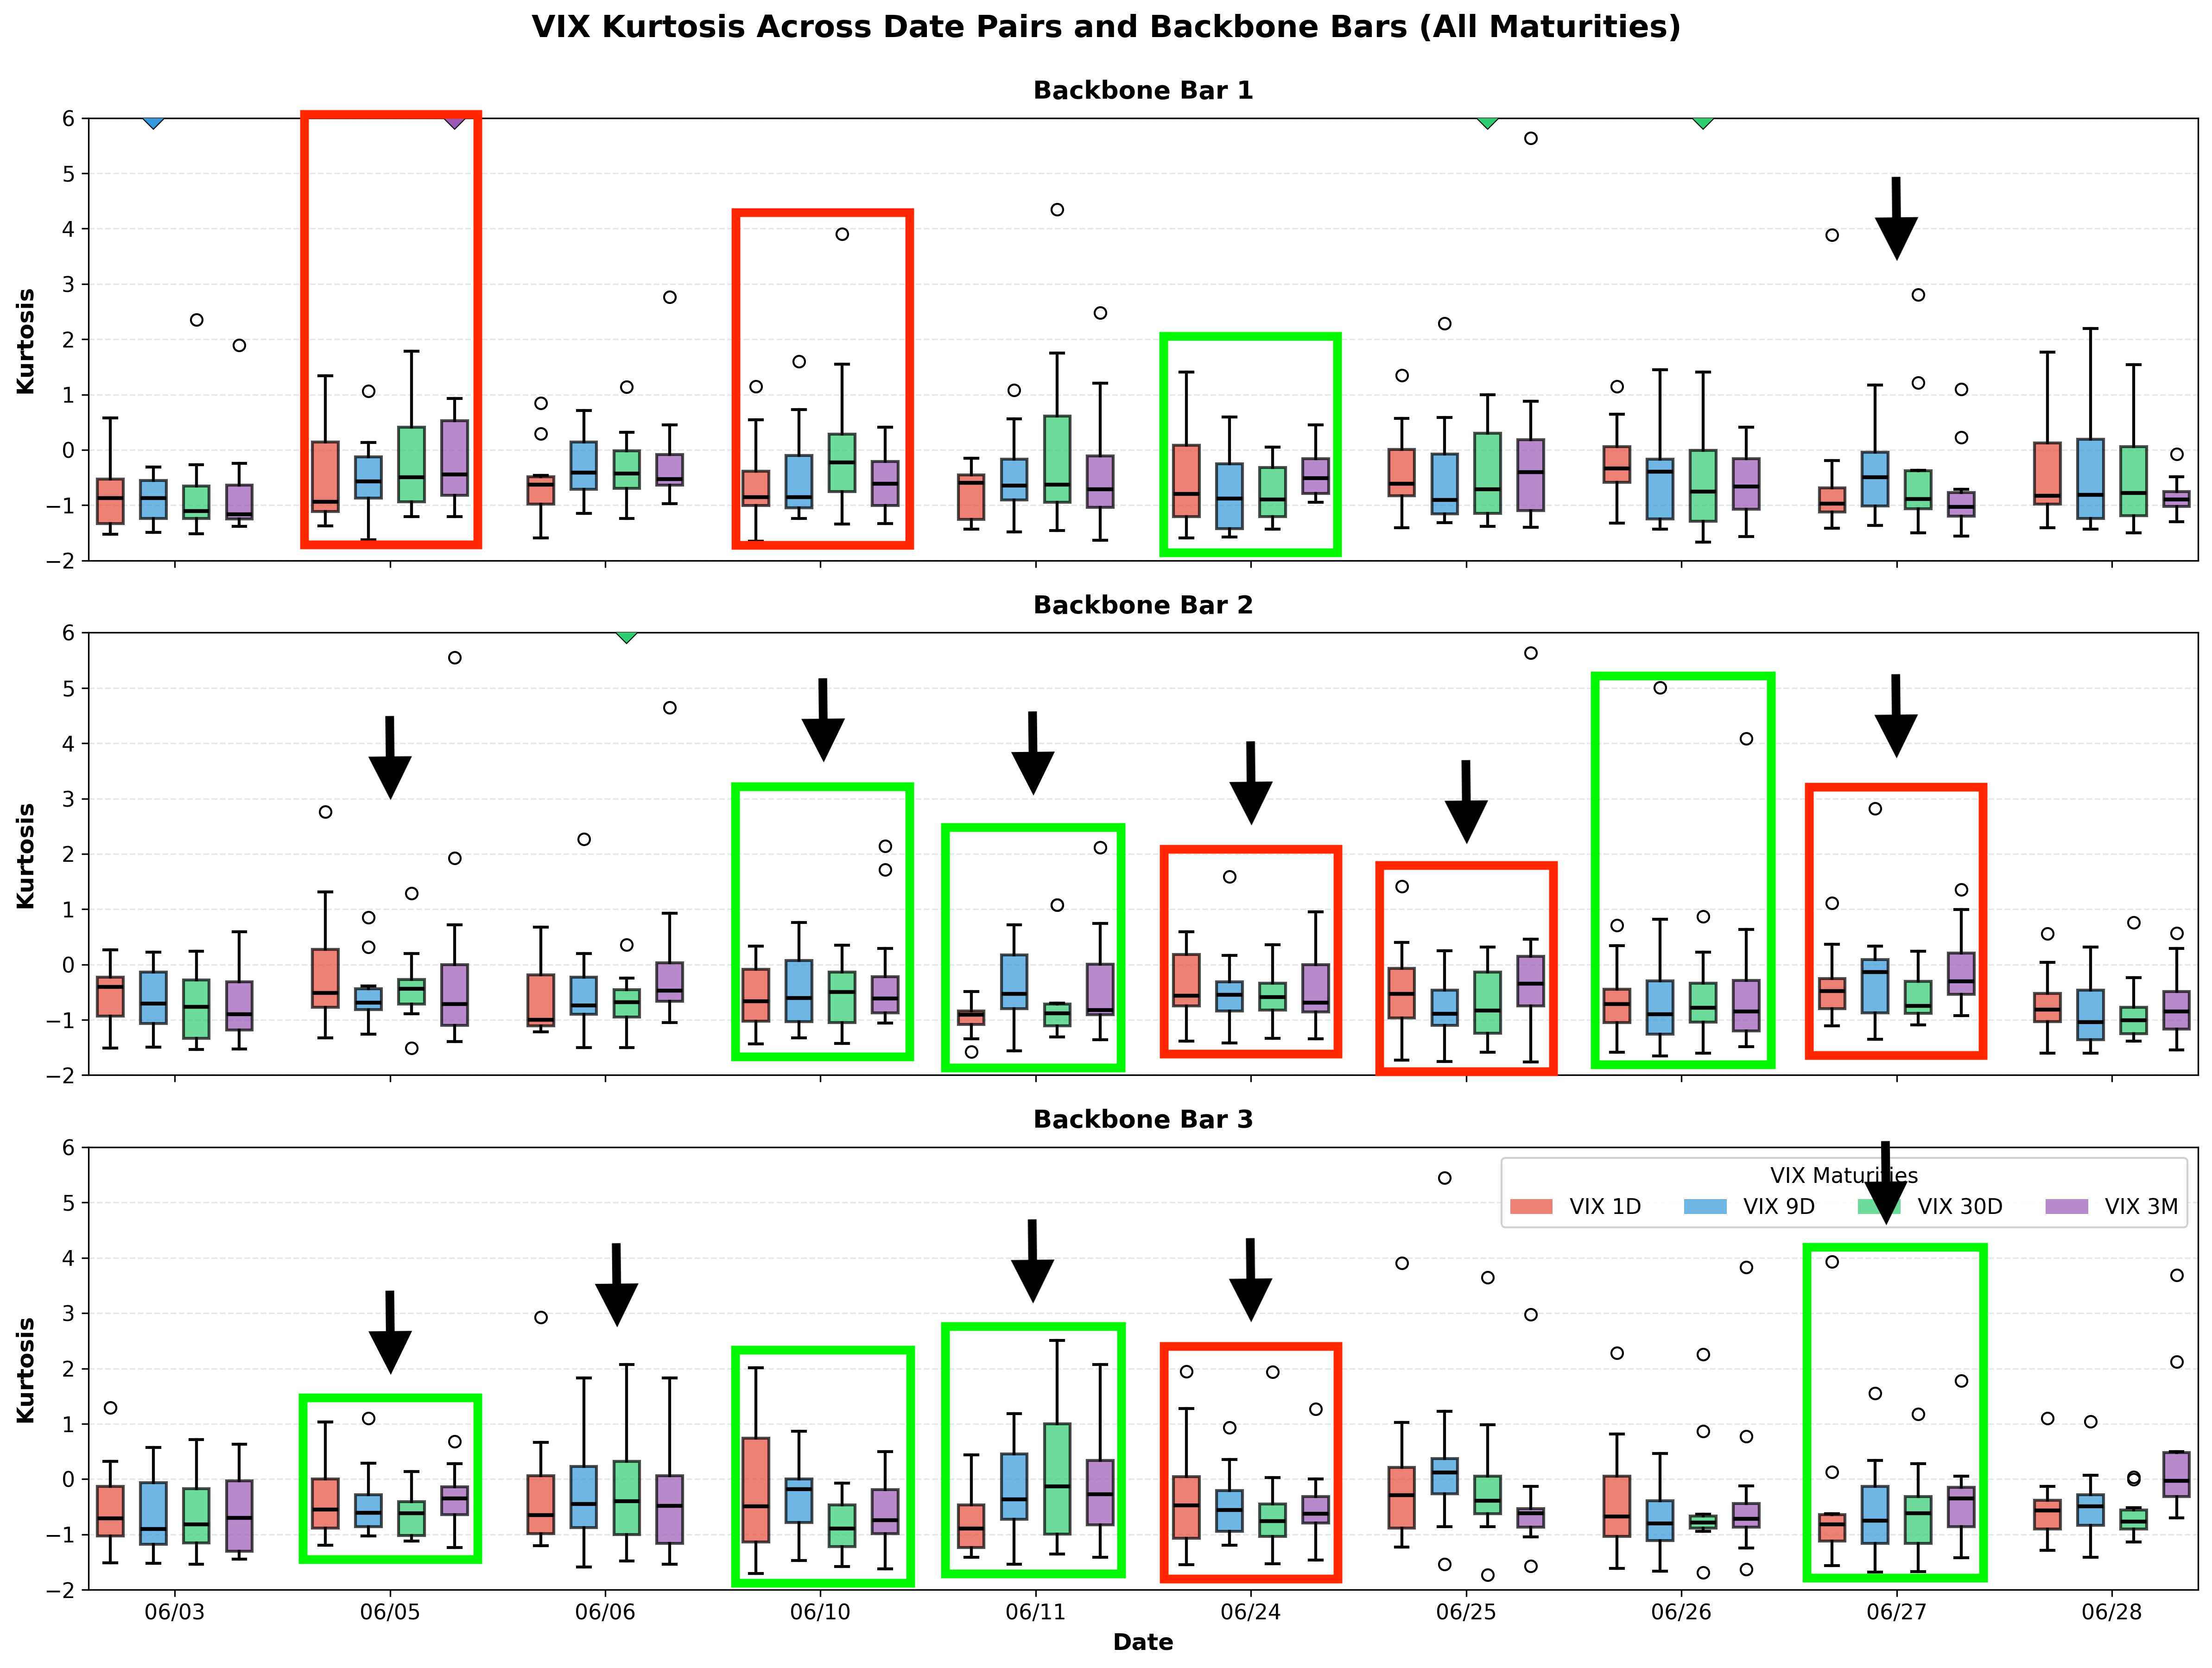
\includegraphics[width=0.9\linewidth]{vix_aggregate_kurtosis_boxplots_marked.png}
\caption{Distribution of the \textbf{kurtosis} of the VIX indices ($VIX_t^{(\tau)}$ for $\tau \in \{ \text{1d}, \text{9d}, \text{30d}, \text{3m} \}$) computed on each adapter bar and aggregated at the backbone bar level. See Figure~\ref{fig:sequential_boxplot_intc_data} for the interpretation of the markers.}
\label{fig:vix_aggregate_kurtosis}
\end{figure}

\begin{figure}[ht!]
\centering

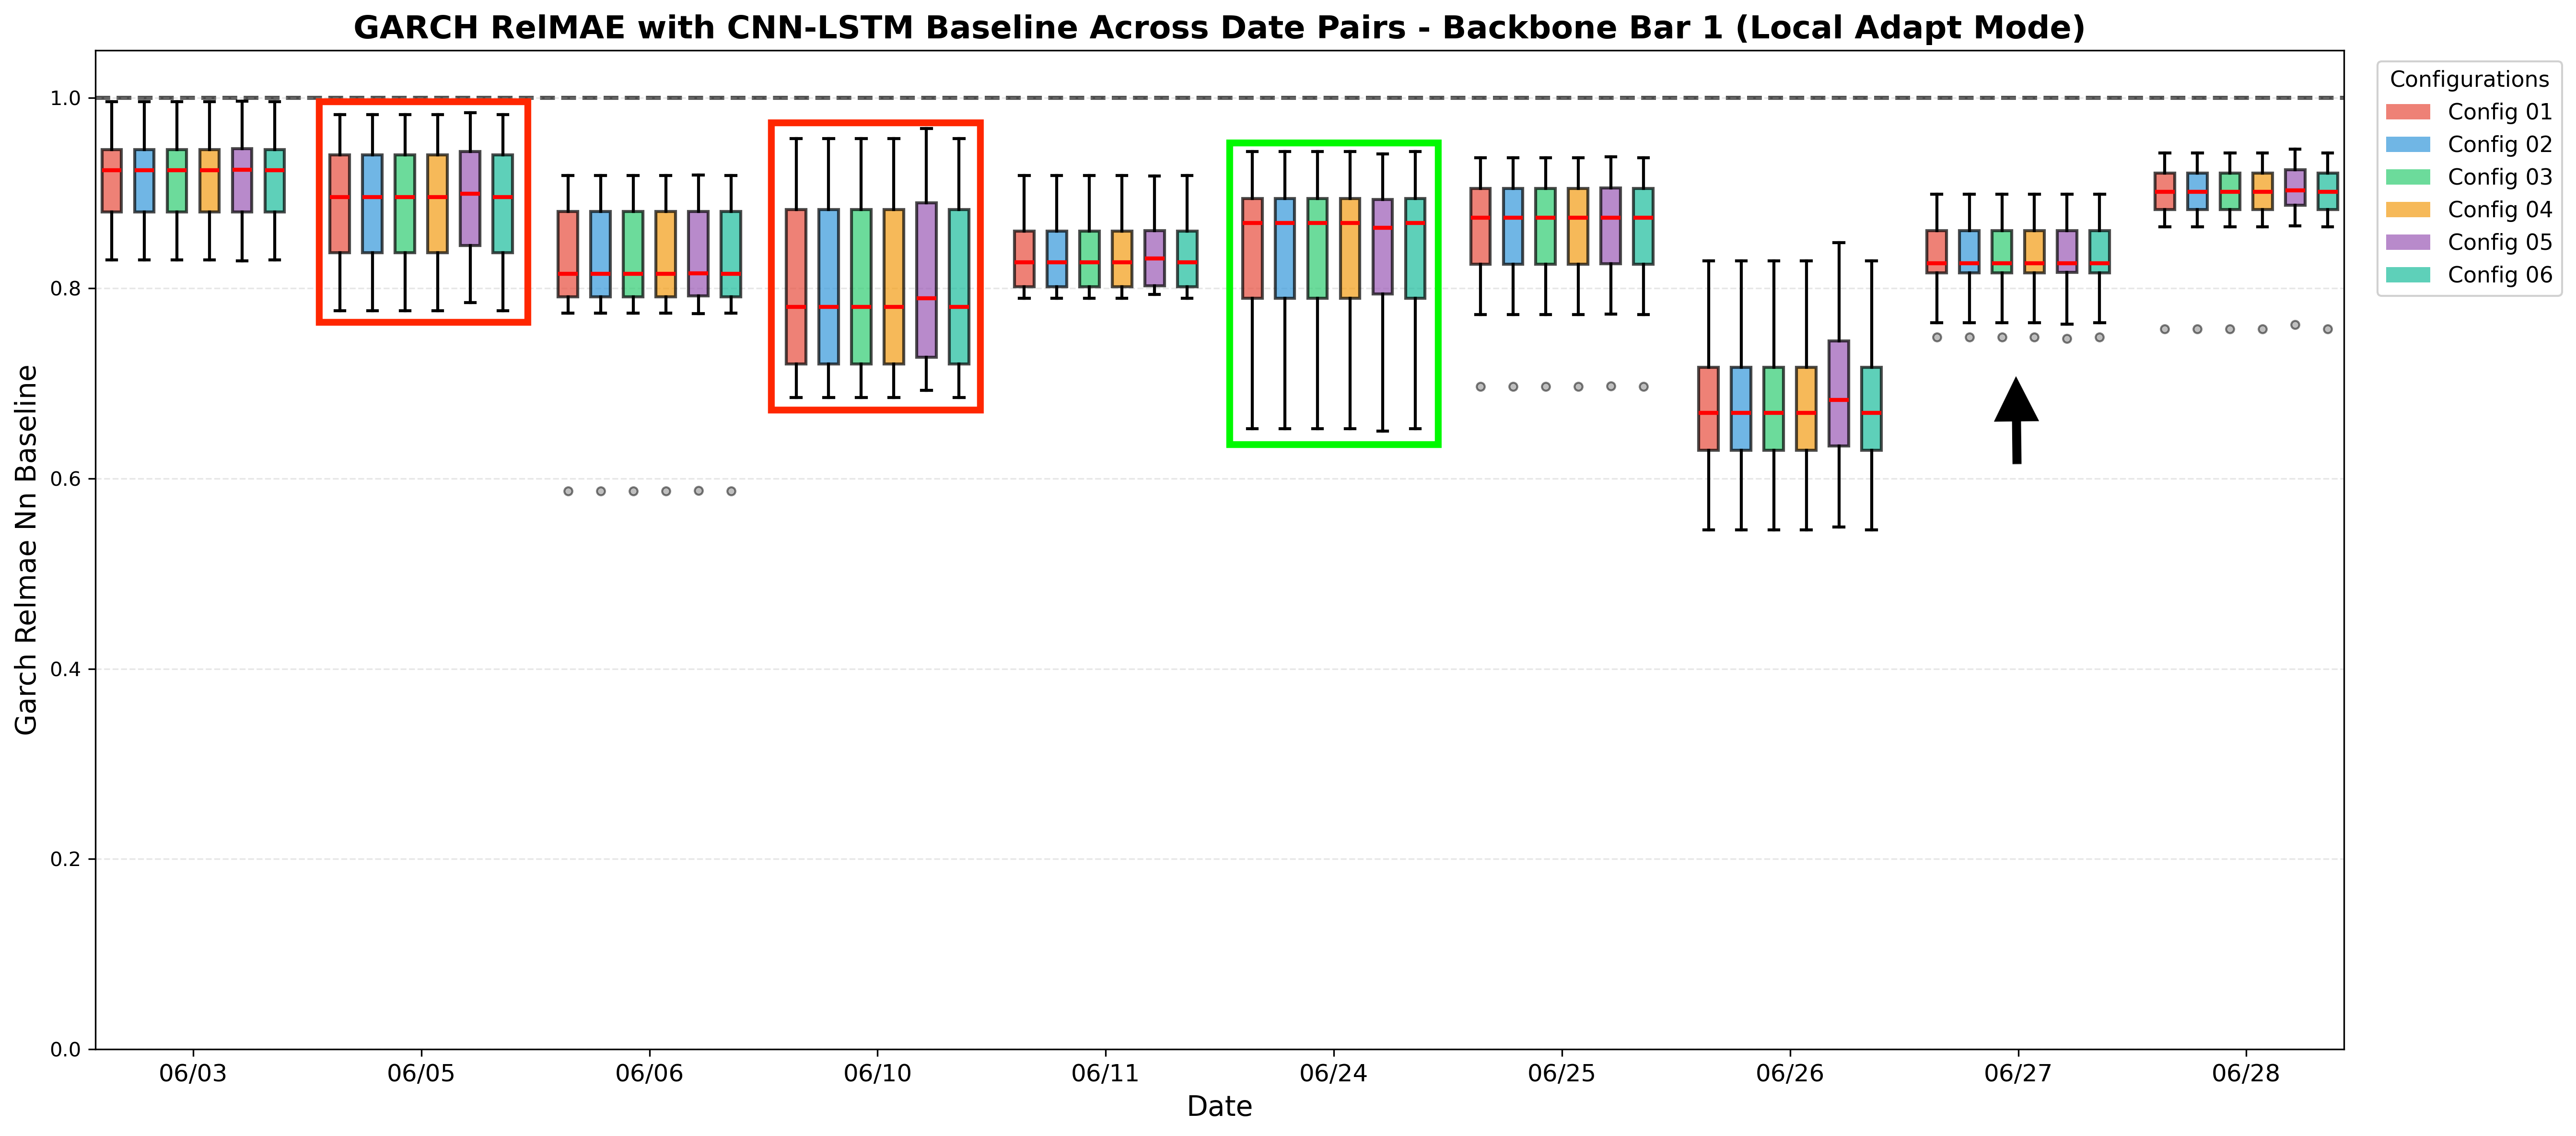
\includegraphics[width=0.9\linewidth]{sequential_boxplot_bb_000_nn_baseline_marked.png}
\vspace{0.5em}
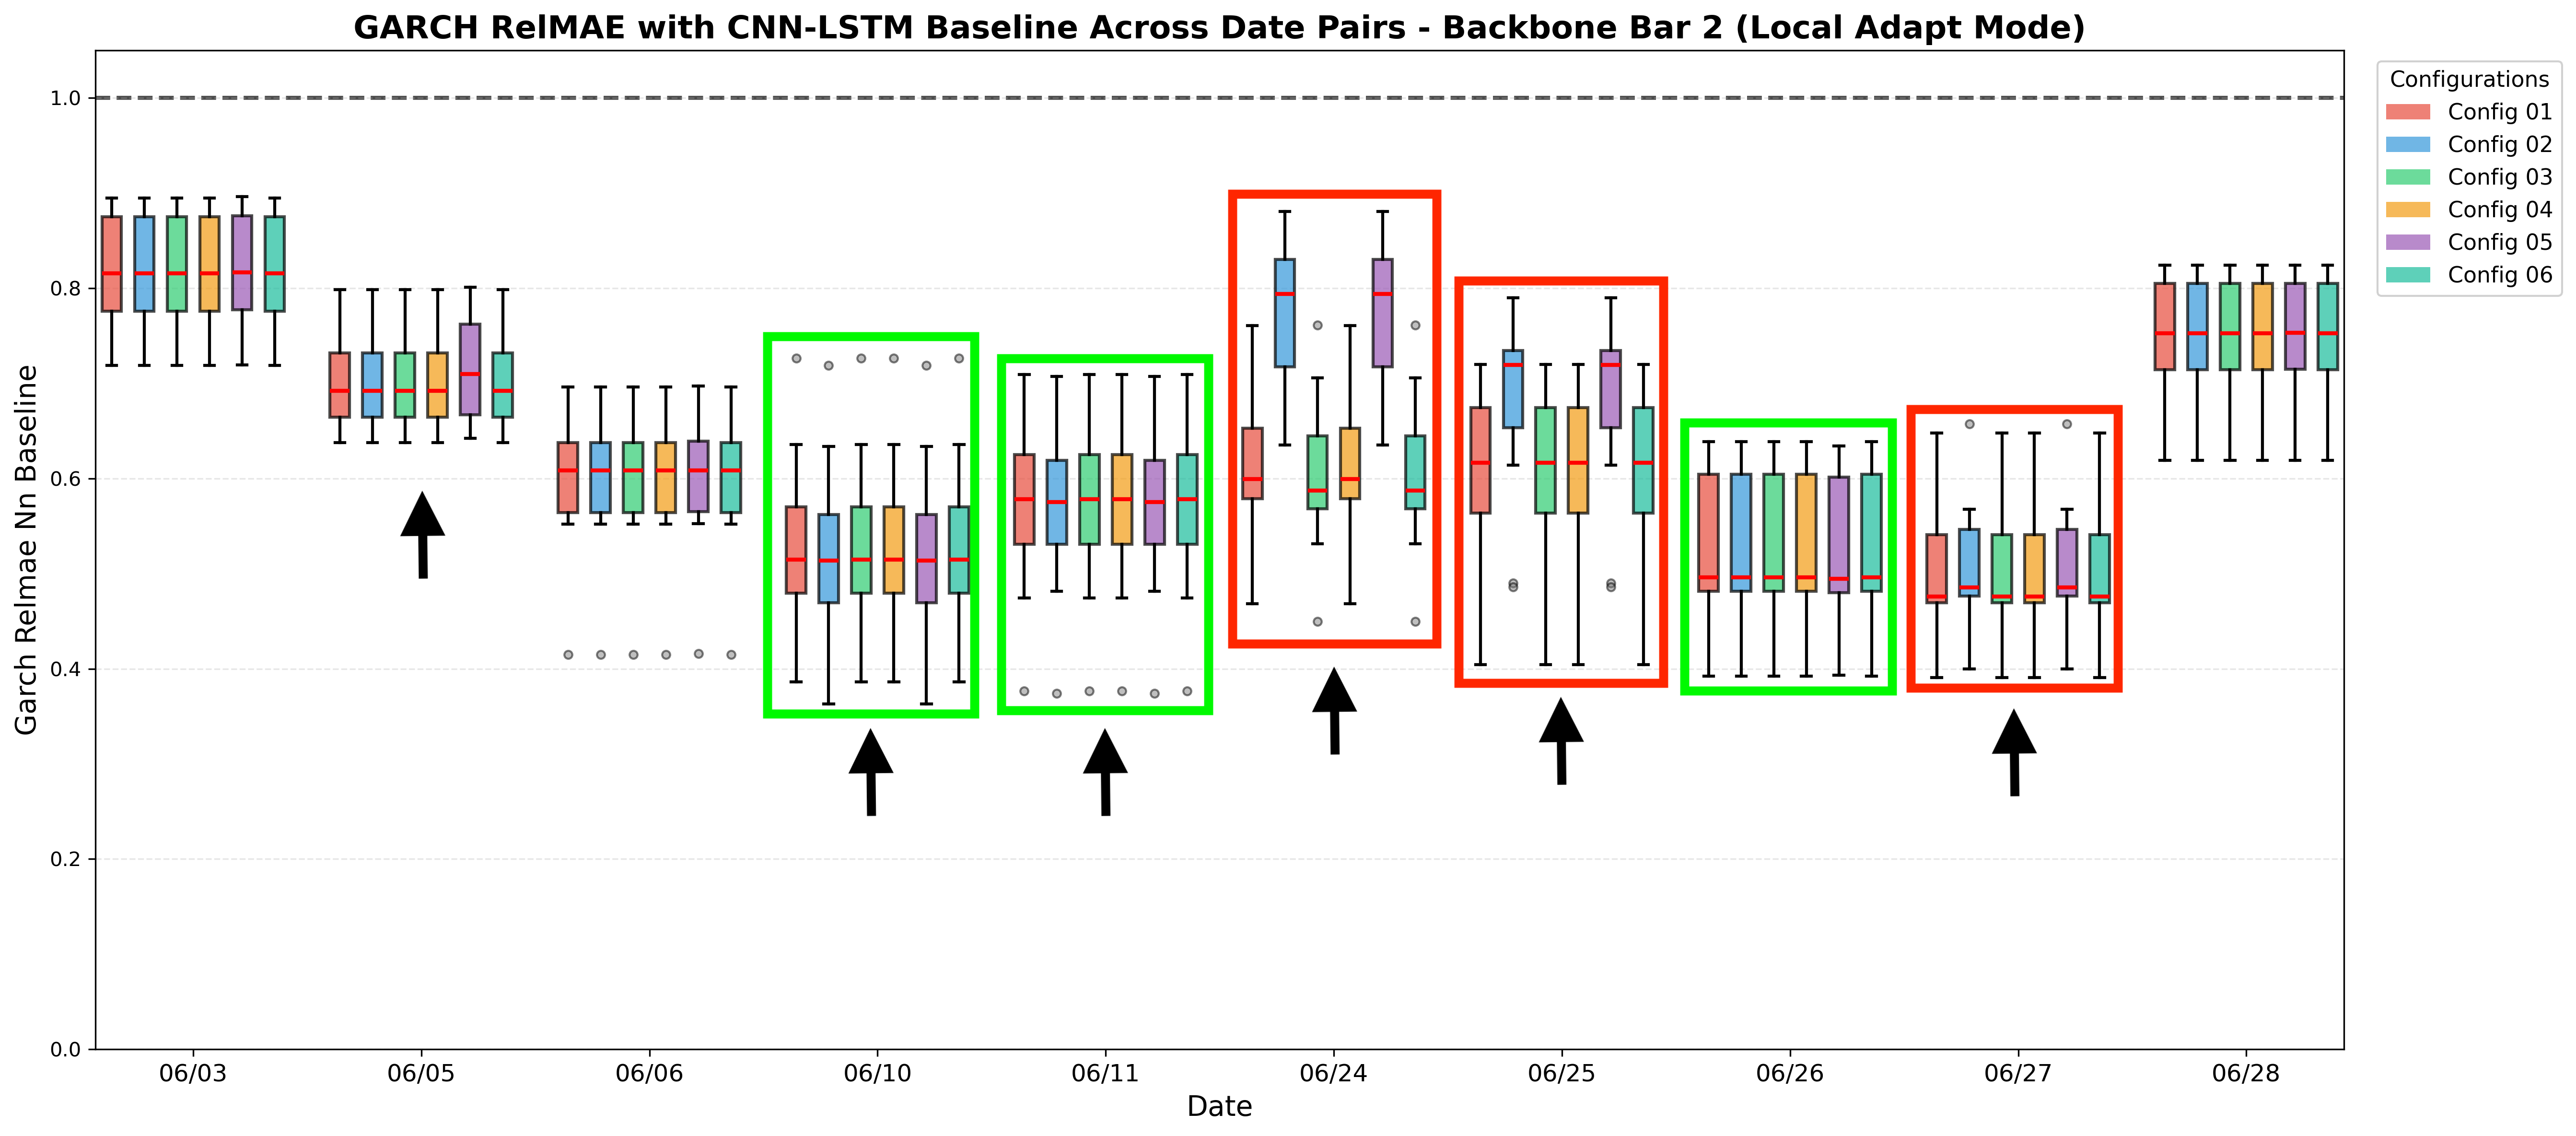
\includegraphics[width=0.9\linewidth]{sequential_boxplot_bb_001_nn_baseline_marked.png}
\vspace{0.5em}
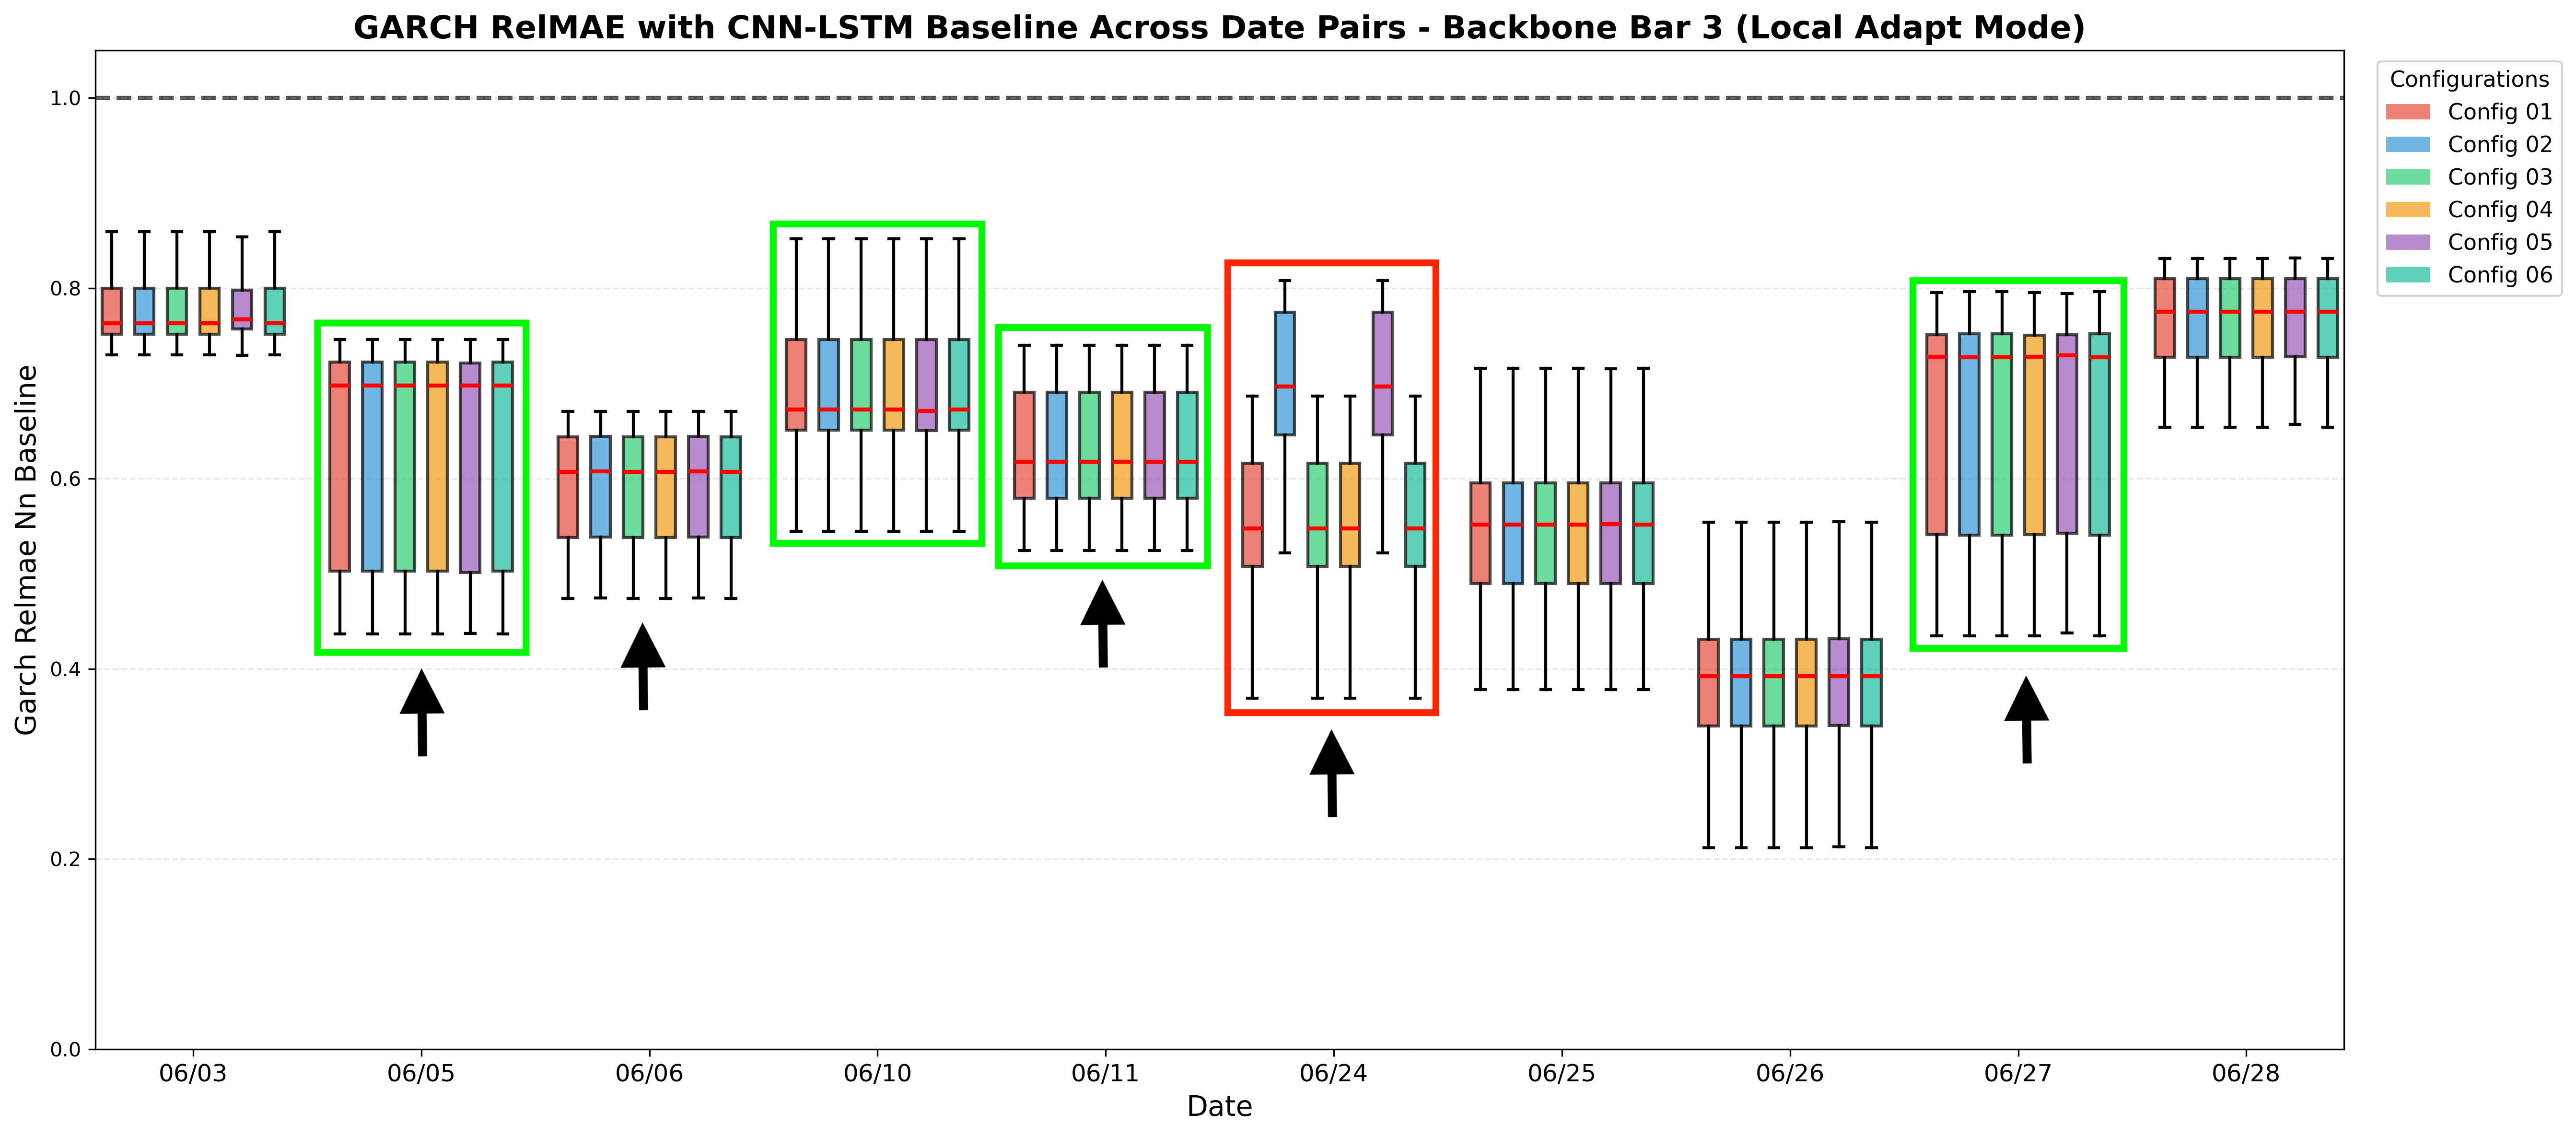
\includegraphics[width=0.9\linewidth]{sequential_boxplot_bb_002_nn_baseline_marked.png}

\caption{Sequential RelMAE boxplots for the INTC dataset across date pairs in Local Adapt mode using the raw CNN-LSTM imputation as the baseline (dashed line at 1.00). Top: Backbone Bar 1; Middle: Backbone Bar 2; Bottom: Backbone Bar 3. See Figure~\ref{fig:sequential_boxplot_intc_data} for the interpretation of the markers (arrows and rectangles).}
\label{fig:sequential_boxplot_intc_data_nn_baseline}
\end{figure}

% \begin{figure}[htb]
%   \centering
%   \includegraphics[width=4in]{param_series_PL3_04.png}
%   \caption{Evolution of parameter estimates for configuration \texttt{PL3\_04}. Blue lines denote combined estimates, while red dashed lines denote bar-specific estimates across adapter bars.}
%   \label{fig:param_series_pl3_04}
% \end{figure}

% \begin{figure}[htb]
%   \centering
%   \includegraphics[width=\linewidth]{armax_garch_corridor_M_03.png}
%   \caption{ARMAX–GARCH-DeepLOB corridor for model \texttt{SA\_04}. Cells show bar-specific coefficient magnitudes by adapter bar; asterisks mark statistical significance.}
%   \label{fig:armax_garch_corridor_M_03}
% \end{figure}


% \begin{figure}[htb]
%     \centering
%     \includegraphics[height=5in]{correlation_matrix_heatmap.png}  
%     \caption{Correlation matrix heatmap}
%     \label{fig:correlation_matrix}
% \end{figure}

% \begin{figure}[htb]
%     \centering
%     \includegraphics[height=4.5in]{arma_garch_coef_corridor.png}  
%     \caption{Corridor plot of purely endogenous ARMA(1, 1)-GARCH(1, 1) model. The numerical methods failed to converge on window 39.}
%     \label{fig:arma_garch_corridor}
% \end{figure}

% \begin{figure}[htb]
%     \centering
%     \includegraphics[height=4.5in]{reg_coef_corridor.png}  
%     \caption{Corridor plot of LASSO coefficients applied to the residuals of the purely endogenous model. Significant coefficients are indicated with $1$ in the corresponding tile.}
%     \label{fig:lasso_ols_corridor}
% \end{figure}

% \begin{figure}[htb]
%     \centering
%     \includegraphics[height=4in]{pos_neg_vs_sig_coefs.png} 
%     \caption{Count of windows where the coefficient is selected by the LASSO model (presence score) vs count of windows where the coefficient is statistically significant following the OLS regression.}
%     \label{fig:lasso_ols_scores}
% \end{figure}


% \begin{figure}[htb]
%     \centering
%     \includegraphics[height=4.5in]{armax_garch_coef_corridor.png} 
%     \caption{Corridor plot of the local coefficients of the Hybrid ARMAX(1, 1)-GARCH(1, 1) model. The optimization algorithms fail to converge on windows $3$ and $39$.}
%     \label{fig:armax_garch_corridor}
% \end{figure}


% \begin{figure}[htb]
%     \centering
%     \includegraphics[height=4in]{armax_garch_coef_evolution.png} 
%     \caption{Time series plot of the local ($\hat{\theta^{(i)}}$) and combined ($\hat{\theta^{(1 : i)}}$) parameter estimates.}
%     \label{fig:armax_garch_evolution}
% \end{figure}

% \begin{figure}[htb]
%     \centering
%     \includegraphics[height=5in]{gof_corridor.png} 
%     \caption{Goodness of fit tests corridor}
%     \label{fig:gof_corridor}
% \end{figure}

% \begin{figure}[htb]
%     \centering
%     \includegraphics[height=5in]{ccf_std_resid_ofi_itv.png} 
%     \caption{Cross correlation function of the Hybrid ARMAX-GARCH-DeepLOB model covariates.}
%     \label{fig:ccf_armax_garch}
% \end{figure}



% \begin{figure}[htb]
%     \centering
%     \includegraphics[height=4.5in]{armax_garch_coef_corridor_dl.png} 
%     \caption{Corridor plot of the local coefficients of the Hybrid ARMAX(1, 1)-GARCH(1, 1) model with distributed lags. The optimization algorithms fail to converge on windows $3$ and $39$.}
%     \label{fig:armax_garch_corridor_dl}
% \end{figure}


% \begin{figure}[htb]
%     \centering
%     \includegraphics[height=4in]{armax_garch_coef_evolution_dl.png} 
%     \caption{Time series plot of the local ($\hat{\theta^{(i)}}$) and combined ($\hat{\theta^{(1 : i)}}$) parameter estimates.}
%     \label{fig:armax_garch_evolution_dl}
% \end{figure}

% \begin{figure}[htb]
%     \centering
%     \includegraphics[height=5in]{gof_corridor_dl.png} 
%     \caption{Goodness of fit tests corridor}
%     \label{fig:gof_corridor_dl}
% \end{figure}

% \begin{figure}[htb]
%     \centering
%     \includegraphics[height=5in]{ccf_std_resid_ofi_itv_dl.png} 
%     \caption{Cross correlation function of the Hybrid ARMAX-GARCH-DeepLOB with distributed lags model covariates.}
%     \label{fig:ccf_armax_garch_dl}
% \end{figure}

\clearpage

\bibliographystyle{plainnat}
\bibliography{references}

\newpage

\end{document}
